\documentclass{article} % For LaTeX2e
\usepackage{iclr2021_conference,times}

% Optional math commands from https://github.com/goodfeli/dlbook_notation.
%%%%% NEW MATH DEFINITIONS %%%%%

\usepackage{amsmath,amsfonts,bm}

% Mark sections of captions for referring to divisions of figures
\newcommand{\figleft}{{\em (Left)}}
\newcommand{\figcenter}{{\em (Center)}}
\newcommand{\figright}{{\em (Right)}}
\newcommand{\figtop}{{\em (Top)}}
\newcommand{\figbottom}{{\em (Bottom)}}
\newcommand{\captiona}{{\em (a)}}
\newcommand{\captionb}{{\em (b)}}
\newcommand{\captionc}{{\em (c)}}
\newcommand{\captiond}{{\em (d)}}

% Highlight a newly defined term
\newcommand{\newterm}[1]{{\bf #1}}


% Figure reference, lower-case.
\def\figref#1{figure~\ref{#1}}
% Figure reference, capital. For start of sentence
\def\Figref#1{Figure~\ref{#1}}
\def\twofigref#1#2{figures \ref{#1} and \ref{#2}}
\def\quadfigref#1#2#3#4{figures \ref{#1}, \ref{#2}, \ref{#3} and \ref{#4}}
% Section reference, lower-case.
\def\secref#1{section~\ref{#1}}
% Section reference, capital.
\def\Secref#1{Section~\ref{#1}}
% Reference to two sections.
\def\twosecrefs#1#2{sections \ref{#1} and \ref{#2}}
% Reference to three sections.
\def\secrefs#1#2#3{sections \ref{#1}, \ref{#2} and \ref{#3}}
% Reference to an equation, lower-case.
\def\eqref#1{equation~\ref{#1}}
% Reference to an equation, upper case
\def\Eqref#1{Equation~\ref{#1}}
% A raw reference to an equation---avoid using if possible
\def\plaineqref#1{\ref{#1}}
% Reference to a chapter, lower-case.
\def\chapref#1{chapter~\ref{#1}}
% Reference to an equation, upper case.
\def\Chapref#1{Chapter~\ref{#1}}
% Reference to a range of chapters
\def\rangechapref#1#2{chapters\ref{#1}--\ref{#2}}
% Reference to an algorithm, lower-case.
\def\algref#1{algorithm~\ref{#1}}
% Reference to an algorithm, upper case.
\def\Algref#1{Algorithm~\ref{#1}}
\def\twoalgref#1#2{algorithms \ref{#1} and \ref{#2}}
\def\Twoalgref#1#2{Algorithms \ref{#1} and \ref{#2}}
% Reference to a part, lower case
\def\partref#1{part~\ref{#1}}
% Reference to a part, upper case
\def\Partref#1{Part~\ref{#1}}
\def\twopartref#1#2{parts \ref{#1} and \ref{#2}}

\def\ceil#1{\lceil #1 \rceil}
\def\floor#1{\lfloor #1 \rfloor}
\def\1{\bm{1}}
\newcommand{\train}{\mathcal{D}}
\newcommand{\valid}{\mathcal{D_{\mathrm{valid}}}}
\newcommand{\test}{\mathcal{D_{\mathrm{test}}}}

\def\eps{{\epsilon}}


% Random variables
\def\reta{{\textnormal{$\eta$}}}
\def\ra{{\textnormal{a}}}
\def\rb{{\textnormal{b}}}
\def\rc{{\textnormal{c}}}
\def\rd{{\textnormal{d}}}
\def\re{{\textnormal{e}}}
\def\rf{{\textnormal{f}}}
\def\rg{{\textnormal{g}}}
\def\rh{{\textnormal{h}}}
\def\ri{{\textnormal{i}}}
\def\rj{{\textnormal{j}}}
\def\rk{{\textnormal{k}}}
\def\rl{{\textnormal{l}}}
% rm is already a command, just don't name any random variables m
\def\rn{{\textnormal{n}}}
\def\ro{{\textnormal{o}}}
\def\rp{{\textnormal{p}}}
\def\rq{{\textnormal{q}}}
\def\rr{{\textnormal{r}}}
\def\rs{{\textnormal{s}}}
\def\rt{{\textnormal{t}}}
\def\ru{{\textnormal{u}}}
\def\rv{{\textnormal{v}}}
\def\rw{{\textnormal{w}}}
\def\rx{{\textnormal{x}}}
\def\ry{{\textnormal{y}}}
\def\rz{{\textnormal{z}}}

% Random vectors
\def\rvepsilon{{\mathbf{\epsilon}}}
\def\rvtheta{{\mathbf{\theta}}}
\def\rva{{\mathbf{a}}}
\def\rvb{{\mathbf{b}}}
\def\rvc{{\mathbf{c}}}
\def\rvd{{\mathbf{d}}}
\def\rve{{\mathbf{e}}}
\def\rvf{{\mathbf{f}}}
\def\rvg{{\mathbf{g}}}
\def\rvh{{\mathbf{h}}}
\def\rvu{{\mathbf{i}}}
\def\rvj{{\mathbf{j}}}
\def\rvk{{\mathbf{k}}}
\def\rvl{{\mathbf{l}}}
\def\rvm{{\mathbf{m}}}
\def\rvn{{\mathbf{n}}}
\def\rvo{{\mathbf{o}}}
\def\rvp{{\mathbf{p}}}
\def\rvq{{\mathbf{q}}}
\def\rvr{{\mathbf{r}}}
\def\rvs{{\mathbf{s}}}
\def\rvt{{\mathbf{t}}}
\def\rvu{{\mathbf{u}}}
\def\rvv{{\mathbf{v}}}
\def\rvw{{\mathbf{w}}}
\def\rvx{{\mathbf{x}}}
\def\rvy{{\mathbf{y}}}
\def\rvz{{\mathbf{z}}}

% Elements of random vectors
\def\erva{{\textnormal{a}}}
\def\ervb{{\textnormal{b}}}
\def\ervc{{\textnormal{c}}}
\def\ervd{{\textnormal{d}}}
\def\erve{{\textnormal{e}}}
\def\ervf{{\textnormal{f}}}
\def\ervg{{\textnormal{g}}}
\def\ervh{{\textnormal{h}}}
\def\ervi{{\textnormal{i}}}
\def\ervj{{\textnormal{j}}}
\def\ervk{{\textnormal{k}}}
\def\ervl{{\textnormal{l}}}
\def\ervm{{\textnormal{m}}}
\def\ervn{{\textnormal{n}}}
\def\ervo{{\textnormal{o}}}
\def\ervp{{\textnormal{p}}}
\def\ervq{{\textnormal{q}}}
\def\ervr{{\textnormal{r}}}
\def\ervs{{\textnormal{s}}}
\def\ervt{{\textnormal{t}}}
\def\ervu{{\textnormal{u}}}
\def\ervv{{\textnormal{v}}}
\def\ervw{{\textnormal{w}}}
\def\ervx{{\textnormal{x}}}
\def\ervy{{\textnormal{y}}}
\def\ervz{{\textnormal{z}}}

% Random matrices
\def\rmA{{\mathbf{A}}}
\def\rmB{{\mathbf{B}}}
\def\rmC{{\mathbf{C}}}
\def\rmD{{\mathbf{D}}}
\def\rmE{{\mathbf{E}}}
\def\rmF{{\mathbf{F}}}
\def\rmG{{\mathbf{G}}}
\def\rmH{{\mathbf{H}}}
\def\rmI{{\mathbf{I}}}
\def\rmJ{{\mathbf{J}}}
\def\rmK{{\mathbf{K}}}
\def\rmL{{\mathbf{L}}}
\def\rmM{{\mathbf{M}}}
\def\rmN{{\mathbf{N}}}
\def\rmO{{\mathbf{O}}}
\def\rmP{{\mathbf{P}}}
\def\rmQ{{\mathbf{Q}}}
\def\rmR{{\mathbf{R}}}
\def\rmS{{\mathbf{S}}}
\def\rmT{{\mathbf{T}}}
\def\rmU{{\mathbf{U}}}
\def\rmV{{\mathbf{V}}}
\def\rmW{{\mathbf{W}}}
\def\rmX{{\mathbf{X}}}
\def\rmY{{\mathbf{Y}}}
\def\rmZ{{\mathbf{Z}}}

% Elements of random matrices
\def\ermA{{\textnormal{A}}}
\def\ermB{{\textnormal{B}}}
\def\ermC{{\textnormal{C}}}
\def\ermD{{\textnormal{D}}}
\def\ermE{{\textnormal{E}}}
\def\ermF{{\textnormal{F}}}
\def\ermG{{\textnormal{G}}}
\def\ermH{{\textnormal{H}}}
\def\ermI{{\textnormal{I}}}
\def\ermJ{{\textnormal{J}}}
\def\ermK{{\textnormal{K}}}
\def\ermL{{\textnormal{L}}}
\def\ermM{{\textnormal{M}}}
\def\ermN{{\textnormal{N}}}
\def\ermO{{\textnormal{O}}}
\def\ermP{{\textnormal{P}}}
\def\ermQ{{\textnormal{Q}}}
\def\ermR{{\textnormal{R}}}
\def\ermS{{\textnormal{S}}}
\def\ermT{{\textnormal{T}}}
\def\ermU{{\textnormal{U}}}
\def\ermV{{\textnormal{V}}}
\def\ermW{{\textnormal{W}}}
\def\ermX{{\textnormal{X}}}
\def\ermY{{\textnormal{Y}}}
\def\ermZ{{\textnormal{Z}}}

% Vectors
\def\vzero{{\bm{0}}}
\def\vone{{\bm{1}}}
\def\vmu{{\bm{\mu}}}
\def\vtheta{{\bm{\theta}}}
\def\va{{\bm{a}}}
\def\vb{{\bm{b}}}
\def\vc{{\bm{c}}}
\def\vd{{\bm{d}}}
\def\ve{{\bm{e}}}
\def\vf{{\bm{f}}}
\def\vg{{\bm{g}}}
\def\vh{{\bm{h}}}
\def\vi{{\bm{i}}}
\def\vj{{\bm{j}}}
\def\vk{{\bm{k}}}
\def\vl{{\bm{l}}}
\def\vm{{\bm{m}}}
\def\vn{{\bm{n}}}
\def\vo{{\bm{o}}}
\def\vp{{\bm{p}}}
\def\vq{{\bm{q}}}
\def\vr{{\bm{r}}}
\def\vs{{\bm{s}}}
\def\vt{{\bm{t}}}
\def\vu{{\bm{u}}}
\def\vv{{\bm{v}}}
\def\vw{{\bm{w}}}
\def\vx{{\bm{x}}}
\def\vy{{\bm{y}}}
\def\vz{{\bm{z}}}

% Elements of vectors
\def\evalpha{{\alpha}}
\def\evbeta{{\beta}}
\def\evepsilon{{\epsilon}}
\def\evlambda{{\lambda}}
\def\evomega{{\omega}}
\def\evmu{{\mu}}
\def\evpsi{{\psi}}
\def\evsigma{{\sigma}}
\def\evtheta{{\theta}}
\def\eva{{a}}
\def\evb{{b}}
\def\evc{{c}}
\def\evd{{d}}
\def\eve{{e}}
\def\evf{{f}}
\def\evg{{g}}
\def\evh{{h}}
\def\evi{{i}}
\def\evj{{j}}
\def\evk{{k}}
\def\evl{{l}}
\def\evm{{m}}
\def\evn{{n}}
\def\evo{{o}}
\def\evp{{p}}
\def\evq{{q}}
\def\evr{{r}}
\def\evs{{s}}
\def\evt{{t}}
\def\evu{{u}}
\def\evv{{v}}
\def\evw{{w}}
\def\evx{{x}}
\def\evy{{y}}
\def\evz{{z}}

% Matrix
\def\mA{{\bm{A}}}
\def\mB{{\bm{B}}}
\def\mC{{\bm{C}}}
\def\mD{{\bm{D}}}
\def\mE{{\bm{E}}}
\def\mF{{\bm{F}}}
\def\mG{{\bm{G}}}
\def\mH{{\bm{H}}}
\def\mI{{\bm{I}}}
\def\mJ{{\bm{J}}}
\def\mK{{\bm{K}}}
\def\mL{{\bm{L}}}
\def\mM{{\bm{M}}}
\def\mN{{\bm{N}}}
\def\mO{{\bm{O}}}
\def\mP{{\bm{P}}}
\def\mQ{{\bm{Q}}}
\def\mR{{\bm{R}}}
\def\mS{{\bm{S}}}
\def\mT{{\bm{T}}}
\def\mU{{\bm{U}}}
\def\mV{{\bm{V}}}
\def\mW{{\bm{W}}}
\def\mX{{\bm{X}}}
\def\mY{{\bm{Y}}}
\def\mZ{{\bm{Z}}}
\def\mBeta{{\bm{\beta}}}
\def\mPhi{{\bm{\Phi}}}
\def\mLambda{{\bm{\Lambda}}}
\def\mSigma{{\bm{\Sigma}}}

% Tensor
\DeclareMathAlphabet{\mathsfit}{\encodingdefault}{\sfdefault}{m}{sl}
\SetMathAlphabet{\mathsfit}{bold}{\encodingdefault}{\sfdefault}{bx}{n}
\newcommand{\tens}[1]{\bm{\mathsfit{#1}}}
\def\tA{{\tens{A}}}
\def\tB{{\tens{B}}}
\def\tC{{\tens{C}}}
\def\tD{{\tens{D}}}
\def\tE{{\tens{E}}}
\def\tF{{\tens{F}}}
\def\tG{{\tens{G}}}
\def\tH{{\tens{H}}}
\def\tI{{\tens{I}}}
\def\tJ{{\tens{J}}}
\def\tK{{\tens{K}}}
\def\tL{{\tens{L}}}
\def\tM{{\tens{M}}}
\def\tN{{\tens{N}}}
\def\tO{{\tens{O}}}
\def\tP{{\tens{P}}}
\def\tQ{{\tens{Q}}}
\def\tR{{\tens{R}}}
\def\tS{{\tens{S}}}
\def\tT{{\tens{T}}}
\def\tU{{\tens{U}}}
\def\tV{{\tens{V}}}
\def\tW{{\tens{W}}}
\def\tX{{\tens{X}}}
\def\tY{{\tens{Y}}}
\def\tZ{{\tens{Z}}}


% Graph
\def\gA{{\mathcal{A}}}
\def\gB{{\mathcal{B}}}
\def\gC{{\mathcal{C}}}
\def\gD{{\mathcal{D}}}
\def\gE{{\mathcal{E}}}
\def\gF{{\mathcal{F}}}
\def\gG{{\mathcal{G}}}
\def\gH{{\mathcal{H}}}
\def\gI{{\mathcal{I}}}
\def\gJ{{\mathcal{J}}}
\def\gK{{\mathcal{K}}}
\def\gL{{\mathcal{L}}}
\def\gM{{\mathcal{M}}}
\def\gN{{\mathcal{N}}}
\def\gO{{\mathcal{O}}}
\def\gP{{\mathcal{P}}}
\def\gQ{{\mathcal{Q}}}
\def\gR{{\mathcal{R}}}
\def\gS{{\mathcal{S}}}
\def\gT{{\mathcal{T}}}
\def\gU{{\mathcal{U}}}
\def\gV{{\mathcal{V}}}
\def\gW{{\mathcal{W}}}
\def\gX{{\mathcal{X}}}
\def\gY{{\mathcal{Y}}}
\def\gZ{{\mathcal{Z}}}

% Sets
\def\sA{{\mathbb{A}}}
\def\sB{{\mathbb{B}}}
\def\sC{{\mathbb{C}}}
\def\sD{{\mathbb{D}}}
% Don't use a set called E, because this would be the same as our symbol
% for expectation.
\def\sF{{\mathbb{F}}}
\def\sG{{\mathbb{G}}}
\def\sH{{\mathbb{H}}}
\def\sI{{\mathbb{I}}}
\def\sJ{{\mathbb{J}}}
\def\sK{{\mathbb{K}}}
\def\sL{{\mathbb{L}}}
\def\sM{{\mathbb{M}}}
\def\sN{{\mathbb{N}}}
\def\sO{{\mathbb{O}}}
\def\sP{{\mathbb{P}}}
\def\sQ{{\mathbb{Q}}}
\def\sR{{\mathbb{R}}}
\def\sS{{\mathbb{S}}}
\def\sT{{\mathbb{T}}}
\def\sU{{\mathbb{U}}}
\def\sV{{\mathbb{V}}}
\def\sW{{\mathbb{W}}}
\def\sX{{\mathbb{X}}}
\def\sY{{\mathbb{Y}}}
\def\sZ{{\mathbb{Z}}}

% Entries of a matrix
\def\emLambda{{\Lambda}}
\def\emA{{A}}
\def\emB{{B}}
\def\emC{{C}}
\def\emD{{D}}
\def\emE{{E}}
\def\emF{{F}}
\def\emG{{G}}
\def\emH{{H}}
\def\emI{{I}}
\def\emJ{{J}}
\def\emK{{K}}
\def\emL{{L}}
\def\emM{{M}}
\def\emN{{N}}
\def\emO{{O}}
\def\emP{{P}}
\def\emQ{{Q}}
\def\emR{{R}}
\def\emS{{S}}
\def\emT{{T}}
\def\emU{{U}}
\def\emV{{V}}
\def\emW{{W}}
\def\emX{{X}}
\def\emY{{Y}}
\def\emZ{{Z}}
\def\emSigma{{\Sigma}}

% entries of a tensor
% Same font as tensor, without \bm wrapper
\newcommand{\etens}[1]{\mathsfit{#1}}
\def\etLambda{{\etens{\Lambda}}}
\def\etA{{\etens{A}}}
\def\etB{{\etens{B}}}
\def\etC{{\etens{C}}}
\def\etD{{\etens{D}}}
\def\etE{{\etens{E}}}
\def\etF{{\etens{F}}}
\def\etG{{\etens{G}}}
\def\etH{{\etens{H}}}
\def\etI{{\etens{I}}}
\def\etJ{{\etens{J}}}
\def\etK{{\etens{K}}}
\def\etL{{\etens{L}}}
\def\etM{{\etens{M}}}
\def\etN{{\etens{N}}}
\def\etO{{\etens{O}}}
\def\etP{{\etens{P}}}
\def\etQ{{\etens{Q}}}
\def\etR{{\etens{R}}}
\def\etS{{\etens{S}}}
\def\etT{{\etens{T}}}
\def\etU{{\etens{U}}}
\def\etV{{\etens{V}}}
\def\etW{{\etens{W}}}
\def\etX{{\etens{X}}}
\def\etY{{\etens{Y}}}
\def\etZ{{\etens{Z}}}

% The true underlying data generating distribution
\newcommand{\pdata}{p_{\rm{data}}}
% The empirical distribution defined by the training set
\newcommand{\ptrain}{\hat{p}_{\rm{data}}}
\newcommand{\Ptrain}{\hat{P}_{\rm{data}}}
% The model distribution
\newcommand{\pmodel}{p_{\rm{model}}}
\newcommand{\Pmodel}{P_{\rm{model}}}
\newcommand{\ptildemodel}{\tilde{p}_{\rm{model}}}
% Stochastic autoencoder distributions
\newcommand{\pencode}{p_{\rm{encoder}}}
\newcommand{\pdecode}{p_{\rm{decoder}}}
\newcommand{\precons}{p_{\rm{reconstruct}}}

\newcommand{\laplace}{\mathrm{Laplace}} % Laplace distribution

\newcommand{\E}{\mathbb{E}}
\newcommand{\Ls}{\mathcal{L}}
\newcommand{\R}{\mathbb{R}}
\newcommand{\emp}{\tilde{p}}
\newcommand{\lr}{\alpha}
\newcommand{\reg}{\lambda}
\newcommand{\rect}{\mathrm{rectifier}}
\newcommand{\softmax}{\mathrm{softmax}}
\newcommand{\sigmoid}{\sigma}
\newcommand{\softplus}{\zeta}
\newcommand{\KL}{D_{\mathrm{KL}}}
\newcommand{\Var}{\mathrm{Var}}
\newcommand{\standarderror}{\mathrm{SE}}
\newcommand{\Cov}{\mathrm{Cov}}
% Wolfram Mathworld says $L^2$ is for function spaces and $\ell^2$ is for vectors
% But then they seem to use $L^2$ for vectors throughout the site, and so does
% wikipedia.
\newcommand{\normlzero}{L^0}
\newcommand{\normlone}{L^1}
\newcommand{\normltwo}{L^2}
\newcommand{\normlp}{L^p}
\newcommand{\normmax}{L^\infty}

\newcommand{\parents}{Pa} % See usage in notation.tex. Chosen to match Daphne's book.

\DeclareMathOperator*{\argmax}{arg\,max}
\DeclareMathOperator*{\argmin}{arg\,min}

\DeclareMathOperator{\sign}{sign}
\DeclareMathOperator{\Tr}{Tr}
\let\ab\allowbreak


\usepackage{amsmath}
\usepackage{amssymb}
\usepackage{amsthm}
\usepackage{thmtools}
\usepackage{mathtools}
\usepackage{graphicx}
%\usepackage{algpseudocode}
%\usepackage{algorithm}
\usepackage[ruled,vlined,linesnumbered,algosection]{algorithm2e}
\usepackage{blindtext}
\usepackage{setspace}
\usepackage[utf8]{inputenc}
\usepackage[utf8]{vietnam}
\usepackage[center]{caption}
\usepackage[shortlabels]{enumitem}
\usepackage{fancyhdr} % header, footer
\usepackage{hyperref} % loại bỏ border với mục lục và công thức
\usepackage{url}
\usepackage[nonumberlist, nopostdot, nogroupskip]{glossaries}
\usepackage{glossary-superragged}
\usepackage{tikz,tkz-tab}
%\usepackage[style=numeric,sortcites]{biblatex}
%\addbibresource{ref.bib}
%\usepackage[numbers]{natbib}
\usepackage{indentfirst}
\usepackage{multirow}
\usepackage{cancel}


\graphicspath{{./figures/}}

\title{Mô hình sinh dựa trên điểm số bằng \\ phương trình vi phân ngẫu nhiên}


\author{Nguyễn Chí Thanh \\
Khoa Toán - Cơ - Tin học\\
Trường Đại học Khoa học Tự nhiên\\
Đại học Quốc Gia Hà Nội \\
\texttt{nguyenchithanh\_sdh21@hus.edu.vn} \\
}

\newcommand{\fix}{\marginpar{FIX}}
\newcommand{\new}{\marginpar{NEW}}

\iclrfinalcopy % Uncomment for camera-ready version, but NOT for submission.

\begin{document}
\maketitle

\begin{abstract}
    Tạo nhiễu từ dữ liệu là một việc đơn giản, nhưng tạo dữ liệu từ nhiễu được gọi là mô hình sinh.
    Ở đề tài này, ta sẽ trình bày phương trình vi phân ngẫu nhiên (SDE) biến đổi một phân phối dữ liệu phức tạp thành một phân phối tiên nghiệm biết trước trơn và thông suốt bằng cách dần dần thêm nhiễu vào dữ liệu,
    và một phương trình vi phân ngẫu nhiên (SDE) ngược (theo thời gian) biến đổi từ phân phối tiên nghiệm trở lại phân phối dữ liệu một cách từ từ bằng việc loại bỏ dần nhiễu.
    Một điều quan trọng là phương trình vi phân ngược theo thời gian chỉ phụ thuộc vào trường gradient phụ thuộc vào thời gian (được gọi là điểm số) của phân phối dữ liệu bị xáo trộn bởi nhiễu.
    Bằng việc tận dụng những bước tiến trong mô hình sinh dựa trên điểm, ta có thể ước lượng chính xác điểm với mạng neuron, và sử dụng các bộ giải phương trình vi phân ngẫu nhiên (SDE) bằng phương pháp số để sinh ra các mẫu dữ liệu.
    Ta sẽ chỉ ra rằng khung làm việc này bao gồm các cách tiếp cận trước đây về mô hình sinh dựa trên điểm số và các mô hình khuếch tán xác suất, cho phép các thủ tục mới để sinh dữ liệu ra đời với những khả năng mạnh hơn.
    Đặc biệt, ta sẽ giới thiệu một bộ dự đoán - căn chỉnh để căn chỉnh sai lệch trong quá trình biến đổi của phương trình vi phân ngẫu nhiên ngược thời gian được rời rạc hóa.
    Ta cũng thu được một mạng neuron ODE tương đương được lấy mẫu từ cùng phân phối như SDE, nhưng ngoài ra cũng cho phép tính toán chính xác độ hợp lý, và cải thiện độ hiệu quả của quá trình lấy mẫu.
    Ngoài ra, ta cũng cung cấp một cách mới để giải các bài toán ngược với các mô hình dựa trên điểm số, được giải thích với các thí nghiệm trên sinh mẫu dựa trên điều kiện nhãn, vẽ ảnh và tô màu.
    Kết hợp với nhiều bước tiến về các kiến trúc mô hình, ta đã đạt kỷ lục với việc sinh ảnh trên tập CIFAR-10 với điểm Inception score là 9.89 và FID là 2.20 và độ hợp lý rất tốt 2.99 bits/dim, và thể hiện khả năng sinh ảnh chân thực với ảnh có độ phân giải 1024 $\times$ 1024 lần đầu tiên từ một mô hình sinh dựa trên điểm số.
\end{abstract}

\section{GIỚI THIỆU}

Hai lớp thành công của các mô hình sinh xác suất liên quan đến việc làm biến đổi dữ liệu một cách tuần tự với độ nhiễu tăng dần, sau đó học cách đảo ngược sự biến đổi để tạ thành một mô hình sinh của dữ liệu.
\textit{Score matching with Langevin dynamics} (SMLD) \citep{song2019generative} ước lượng điểm số (ví dụ gradient của log của hàm mật độ xác suất của dữ liệu) tại từng mức nhiễu, sau đó sử dụng động học Langevin để lấy mẫu từ mỗi dãy các mức nhiễu giảm dần trong suốt quá trình sinh dữ liệu.
\textit{Denoising diffusion probabilistic modeling} (DDPM) \citep{sohl2015deep,ho2020denoising} huấn luyện một dãy các mô hình xác suất để đảo ngược từng bước của quá trình bị xáo trộn bởi nhiễu,
sử dụng những kiến thức về dạng chức năng của các phân phối ngược làm cho quá trình huấn luyện dễ dàng hơn.
Trong không gian trạng thái liên tục, DDPM huấn luyện hàm mục tiêu ngầm tính điểm số tại từng mức nhiễu.
Vì vậy, ta gọi hai lớp mô hình này là các \textit{mô hình sinh dựa trên điểm số}.

Các mô hình sinh dựa trên điểm số và các kỹ thuật liên quan \citep{bordes2017learning, goyal2017variational,du2019implicit} đã được chứng minh là hiệu quả trong bài toán sinh ảnh \citep{song2019generative,song2020sliced,ho2020denoising}, âm thanh \citep{chen2020wavegrad,kong2020diffwave}, đồ thị \citep{niu2020permutation} và các khối hình \citep{cai2020learning}.
Để cho phép các phương pháp lấy mẫu mới mở rộng khả năng của các mô hình sinh dựa trên điểm số, ta đề xuất một khung làm việc thống nhất tổng quát hóa các cách tiếp cận trước đó thông qua góc nhìn của phương trình vi phân ngẫu nhiên.

\begin{figure}[h!]
    \centering
    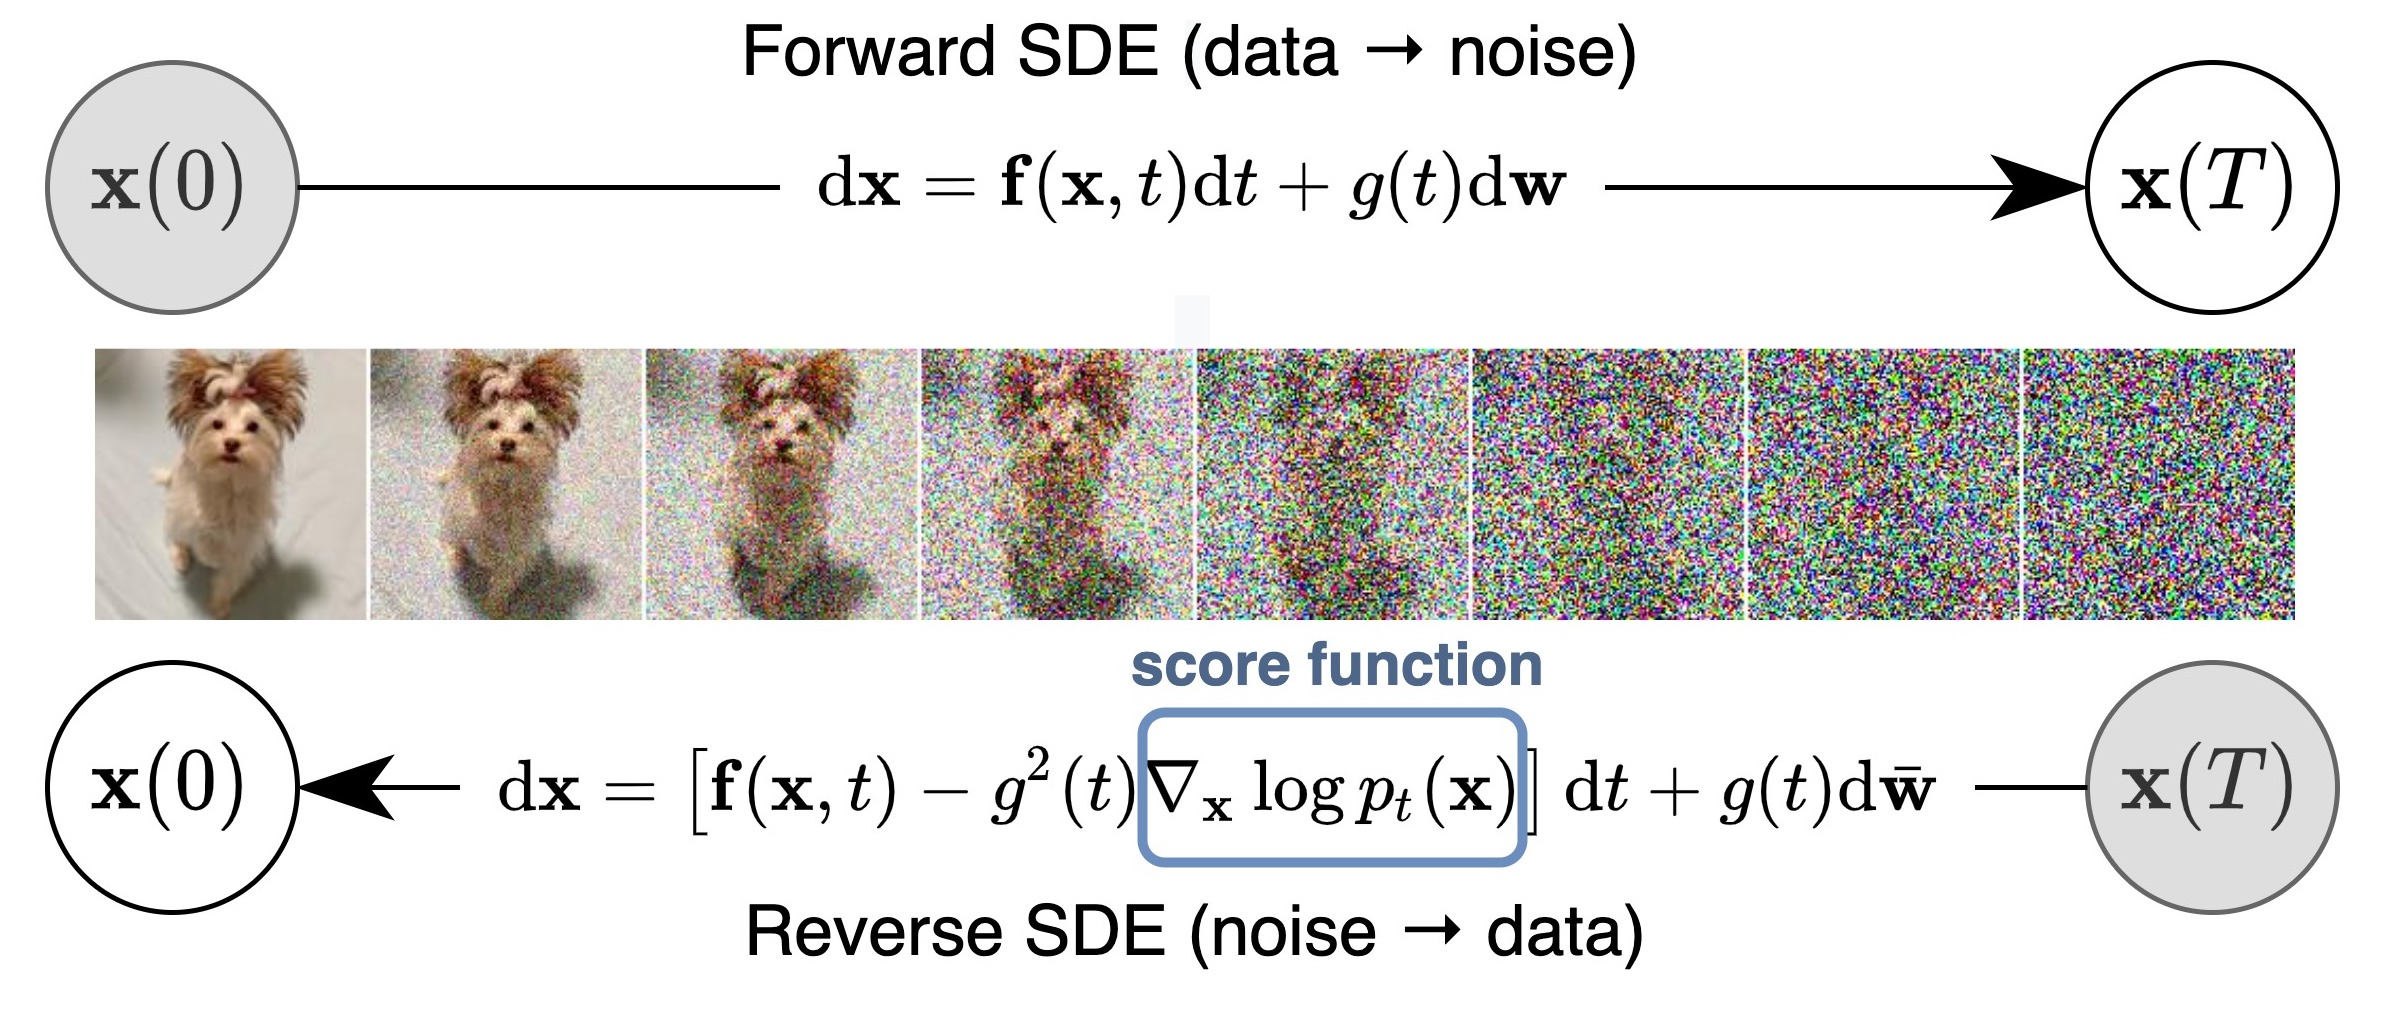
\includegraphics[width=0.8\textwidth]{1.jpg}
    \caption{\textbf{Giải một phương trình SDE đảo ngược thời gian thu được một mô hình sinh dựa trên điểm.}
    Biến đổi dữ liệu thành một phân phối nhiễu đơn giản có thể được thực hiện với một phương trình SDE liên tục theo thời gian.
    Phương trình SDE này có thể được đảo ngược nếu ta biết điểm của phân phối tại từng bước thời gian trung gian, $\nabla_{\bold{x}}\log p_t (\bold{x})$.}
    \label{fig:1}
\end{figure}

Cụ thể, thay vì làm nhiễu với một số hữu hạn của các phân phối nhiễu, ta xét một phân phối biến đổi một cách liên tục theo thời gian tương ứng với quá trình khuếch tán.
Quá trình này khuếch tán dần dần các điểm dữ liệu thành nhiễu ngẫu nhiên và được cho bởi một SDE cho trước không phụ thuộc vào dữ liệu và không có các tham số có thể huấn luyện.
Bằng cách đảo ngược quá trình này, ta có thể biến đổi nhiễu thành dữ liệu một cách trơn cho bài toán sinh mẫu dữ liệu.
Điều quan trọng là quá trình ngược này thỏa mãn SDE ngược theo thời gian \citep{anderson1982reverse}, có thể suy ra từ phương trình SDE thuận được cho bởi điểm số của hàm mật độ xác suất cận biên như là một hàm của thời gian.
Vì vậy ta có thể xấp xỉ SDE ngược thời gian bằng cách huấn luyện một mạng neuron phụ thuộc thời gian để ước lượng điểm số và sau đó tạo ra các mẫu dữ liệu sử dụng các bộ giải SDE bằng phương pháp số.
Ý tưởng chính được trình bày ở hình \ref{fig:1}.

Khung làm việc đề xuất có nhiều đóng góp về mặt lý thuyết và thực tiễn:

\textbf{Lấy mẫu linh hoạt và tính toán độ hợp lý:} Ta có thể sử dụng bất kỳ một bộ giải phương trình SDE đa chức năng nào để tích hợp phương trình SDE đảo ngược thời gian cho bài toán lấy mẫu.
Hơn nữa, ta đề xuất hai phương pháp đặc biệt mà không phù hợp với phương trình SDE nói chung: (i) Bộ lấy mẫu Dự đoán - Căn chỉnh (PC) kết hợp với bộ giải SDE bằng phương pháp số và cách tiếp cận MCMC (Markov Chain Monte Carlo) dựa trên điểm số, như Langevin MCMC \citep{parisi1981correlation} và HMC \citep{neal2011mcmc} và (ii) các bộ lấy mẫu tất định dựa trên dòng xác suất của các phương trình vi phân thường (ODE).
Phương pháp thứ nhất hợp nhất vả cải thiện các phương pháp lấy mẫu hiện có cho các mô hình dựa trên điểm số.
Phương pháp thứ hai cho phép lấy mẫu thích ứng nhanh thông qua một hộp đen là một bộ giải phương trình ODE, các thao tác trên dữ liệu linh hoạt thông qua mã ẩn, mỗi mã có tính duy nhất và điều đáng chú ý ta có thể tính chính xác độ hợp lý.

\textbf{Sinh dữ liệu có điều kiện:} Ta có thể điều chỉnh quá trình sinh dữ liệu bằng cách điều chỉnh các thông tin không có sẵn trong quá trình huấn luyện, bởi vì phương trình SDE đảo ngược thời gian có điều kiện có thể được ước lượng hiệu quả từ các điểm số \textit{không có điều kiện}.
Điều này cho phép các ứng dụng như sinh ảnh có điều kiện về lớp, vẽ ảnh, tô màu cũng như các bài toán ngược khác, tất cả các bài toán trên đều có thể được giải quyết bằng cách sử dụng một mô hình dựa trên điểm số không có điều kiện mà không cần phải huấn luyện lại mô hình.

\textbf{Khung làm việc thống nhất:} Khung làm việc của ta cung cấp một cách thống nhất để khai phá của chỉnh định nhiều phương trình SDE cho việc cải thiện các mô hình sinh dựa trên điểm số.
Các phương pháp của SMLD và DDPM có thể được đưa vào khung làm việc của ta bằng cách rời rạc hóa hai phương trình SDE riêng biệt.
Mặc dù DDPM \citep{ho2020denoising} gần đây đã được báo cáo là có thể đạt được mẫu có chất lượng cao hơn SMLD \citep{song2019generative,song2020improved}, ta chỉ ra điều đó với kiến trúc mạng tốt hơn và các thuật toán lấy mẫu mới cho phép bởi khung làm việc của ta, mô hình sau đó có thể bắt kịp và đạt được đến điểm Inception kỷ lục (9.89) và FID (2.20) trên tập CIFAR-10 cũng như độ chân thực của ảnh có độ phân giải 1024 $\times$ 1024 lần đầu tiên từ một mô hình sinh dựa trên điểm.
Ngoài ra, ta đề xuất một phương trình SDE mới trong khung làm việc của ta thu được độ hợp lý có giá trị 2.99 bits/dim trên tập CIFAR-10, tạo nên một kỷ lục mới cho bài toán này.

\section{Kiến thức nền tảng}

\subsection{Khử nhiều khớp điểm số với động học Langevin (SMLD)}

Đặt $p_{\sigma}(\tilde{\bold{x}} \vert \bold{x}) \vcentcolon = \mathcal{N}(\tilde{\bold{x}};\bold{x}, \sigma^2 \bold{I})$ là một nhân tạo ra nhiễu, và $p_{\sigma}(\tilde{\bold{x}})\vcentcolon = \int p_{\mathrm{data}}(\bold{x}) p_{\sigma}(\tilde{\bold{x}} \vert \bold{x}) d \bold{x}$, với $p_{\mathrm{data}}$ ký hiệu là phân phối dữ liệu.
Ta xét một dãy các mức nhiễu dương $\sigma_{\min} < \sigma_2 < \dots < \sigma_N = \sigma_{\max}$.
Thông thường, $\sigma_{\min}$ đủ nhỏ dể $p_{\sigma_{\min}} \approx p_{\mathrm{data}}(\bold{x})$, và $\sigma_{\max}$ đủ lớn để $p_{\sigma_{\max}}\approx \mathcal{N}(\bold{x}; \bold{0}, \sigma_{\max}^2 \bold{I})$.
\citep{song2019generative} đề xuất huấn luyện một mạng điểm số có điều kiện nhiễu (Noise Conditional Score Network - NCSN), ký hiệu $\bold{s}_{\boldsymbol{\theta}}(\bold{x}, \sigma)$ với một tổng có trọng số của các hàm khớp điểm số khử nhiễu \citep{vincent2011connection}:

\begin{equation} \label{eq:1}
    \boldsymbol{\theta}^{\ast} = \argmin_{\boldsymbol{\theta}} \sum_{i=1}^N \sigma_i^2 \mathbb{E}_{p_{\mathrm{data}}(\bold{x})} \mathbb{E}_{p_{\sigma_i}(\tilde{\bold{x}} \vert \bold{x})} \big\lbrack \lVert \bold{s}_{\boldsymbol{\theta} (\tilde{\bold{x}}, \sigma_i)} - \nabla_{\tilde{\bold{x}}} \log p_{\sigma_i} (\tilde{\bold{x}} \vert \bold{x})  \rVert_2^2 \big\rbrack
\end{equation}

Khi được cho một dữ liệu và một mô hình có kích thước phù hợp, mô hình dựa trên điểm số tối ưu $\bold{s}_{\boldsymbol{\theta}^{\ast}}(\bold{x}, \sigma)$ khớp với $\nabla_{\bold{x}} \log p_{\sigma}(\bold{x})$ tại hầu hết vị trí với $\sigma \in \lbrace \sigma_i \rbrace_{i=1}^N$.
Để lấy mẫu, \citep{song2019generative} chạy M bước của Langevin MCMC để thu được mẫu dữ liệu cho lần lượt từng $p_{\sigma_i}(\bold{x})$:

\begin{equation}
    \bold{x}_i^m = \bold{x}_i^{m-1} + \epsilon_i \bold{s}_{\boldsymbol{\theta}^{\ast}} (\bold{x}_i^{m-1}, \sigma_i) + \sqrt{2 \epsilon_i} \bold{z}_i^m, m = 1, 2, \dots, M
\end{equation}

với $\epsilon_i > 0$ là độ dài bước và $\bold{z}_i^m$ là một biến tuân theo phân phối chuẩn tắc.
Công thức trên được lặp lại cho $i=N, N-1, \dots, 1$ với $\bold{x}_N^0 \sim \mathcal{N}(\bold{x} \vert \bold{0}, \sigma_{\max}^2 \bold{I})$ và $\bold{x}_i^0 = \bold{x}_{i+1}^M$ khi $i < N$. Khi $M \rightarrow \infty$ và $\epsilon_i \rightarrow 0$ với mọi $i, \bold{x}_1^M$ trở thành một mẫu chính xác từ $p_{\sigma_{\min}}(\bold{x})\approx p_{\mathrm{data}}(\bold{x})$ trong một số điều kiện.


\subsection{Mô hình xác suất khuếch tán khử nhiễu (DDPM)}

\citep{sohl2015deep,ho2020denoising} xét một dãy các ngưỡng nhiễu dương $0 < \beta_1, \beta_2, \dots, \beta_N < 1$.
Với từng điểm dữ liệu huấn luyện $\bold{x}_0 \sim p_{\mathrm{data}}(\bold{x})$, một xích Markov rời rạc $\lbrace \bold{x}_1, \bold{x}_2, \dots, \bold{x}_N \rbrace$ được tạo ra sao cho $p(\bold{x}_i \vert \bold{x}_{i-1}) = \mathcal{N}(\bold{x}_i; \sqrt{1-\beta_i} \bold{x}_{i-1}, \beta_i \bold{I})$ và vì vậy $p_{\alpha_i}=\mathcal{N}(\bold{x}_i; \sqrt{\alpha_i}\bold{x}_0, (1-\alpha_i)\bold{I})$,
với $\alpha_i \vcentcolon = \prod_{j=1}^i (1 - \beta_j)$.
Tương tự với SMLD, ta có thể ký hiệu phân phối dữ liệu bị xáo trộn là $p_{\alpha_i}\vcentcolon =  \int p_{\mathrm{data}}(\bold{x}) p_{\alpha_i}(\tilde{\bold{x}} \vert \bold{x}) d \bold{x}$.
Các mức nhiễu được chọn sao cho $\bold{x}_N$ có phân phối xấp xỉ phân phối chuẩn tắc $\mathcal{N}(\bold{0}, \bold{I})$.
Một xích Markov biến phân theo chiều ngược được tham số hóa với $p_{\boldsymbol{\theta}} (\bold{x}_{i-1} \vert \bold{x}_i)=\mathcal{N}\Big(\bold{x}_{i-1}; \dfrac{1}{\sqrt{1-\beta_i}}(\bold{x}_i + \beta_i \bold{s}_{\boldsymbol{\theta}}(\bold{x}_i, i)), \beta_i \bold{I}\Big)$ và được huấn luyện với một biến thể được đánh lại trọng số của cận dưới của độ hợp lý (ELBO):

\begin{equation} \label{eq:3}
    \boldsymbol{\theta}^{\ast} = \argmin_{\boldsymbol{\theta}} \sum_{i=1}^N (1 - \alpha_i) \mathbb{E}_{p_{\mathrm{data}}(\bold{x})} \mathbb{E}_{p_{\alpha_i (\tilde{\bold{x}} vert \bold{x})}} \big \lbrack \lVert \bold{s}_{\boldsymbol{\theta}} (\tilde{\bold{x}}, i) - \nabla_{\tilde{\bold{x}}} \log p_{\alpha_i} (\tilde{\bold{x}} \vert \bold{x}) \rVert_2^2 \big \rbrack
\end{equation}

Sau khi giải phương trình \ref{eq:3} để thu được mô hình tối ưu $\bold{s}_{\boldsymbol{\theta}^{\ast}}(\bold{x}, i)$, các mẫu có thể được tạo ra bằng cách bắt đầu từ một nhiễu tuân theo phân phối chuẩn tắc $\bold{x}_N \sim \mathcal{N}(\bold{0}, \bold{I})$ và sử dụng công thức ước lượng xích Markov ngược sau đây:

\begin{equation} \label{eq:4}
    \bold{x}_{i-1} = \dfrac{1}{\sqrt{1-\beta_i}} \big( \bold{x}_i + \beta_i \bold{s}_{\boldsymbol{\theta}^{\ast}} (\bold{x}_i, i) \big) + \sqrt{\beta_i} \bold{z}_i, i = N, N-1, \dots, 1
\end{equation}

Ta gọi phương pháp này là \textit{ancestral sampling}, khi mà phương pháp này thực hiện lấy mẫu từ một mô hình đồ thị $\prod_{i=1}^N p_{\boldsymbol{\theta}} (\bold{x}_{i-1} \vert \bold{x}_i)$.
Hàm mục tiêu trong công thức \ref{eq:3} là $L_{\mathrm{simple}}$ trong \citep{ho2020denoising} được viết dưới dạng khá tương đồng với công thức \ref{eq:1}.
Cũng như công thức \ref{eq:1}, công thức \ref{eq:3} cũng là tổng có trọng số của các hàm mục tiêu khớp điểm số khử nhiễu, $\nabla_{\bold{x}}\log p_{\alpha_i}(\bold{x})$.
Đáng chú ý là trọng số thứ $i$ được đề cập trong công thức \ref{eq:1} và công thức \ref{eq:3} là $\sigma_i^2$ và $(1-\alpha_i)$ liên quan đến các nhân gây xáo trộn tương ứng trong cùng một dạng chức năng:
$\sigma_i^2 \propto 1/\mathbb{E} \big \lbrack \lVert \nabla_{\bold{x}} \log p_{\sigma_i} (\tilde{\bold{x}} \vert \bold{x}) \rVert_2^2 \big \rbrack$ và $(1-\alpha_i) \propto 1/\mathbb{E} \big \lbrack \lVert \nabla_\bold{x} \log p_{\alpha_i}  (\tilde{\bold{x}} \vert \bold{x})\rVert_2^2 \big \rbrack$

\section{Mô hình sinh dựa trên điểm số với SDE}

Để làm nhiễu hay làm xáo trộn dữ liệu với nhiều mức nhiễu là một chìa khóa dẫn đến thành công của các phương pháp trước đây.
Ta đề xuất tổng quát hóa ý tưởng này hơn nữa trở thành một số vô hạn các mức nhiễu, chẳng hạn phân phối của dữ liệu bị làm nhiễu biến đổi tuân theo một phương trình SDE khi nhiễu tăng dần lên.
Tổng quát của khung làm việc của ta được miêu tả trong hình \ref{fig:2}


\begin{figure}[h!]
    \centering
    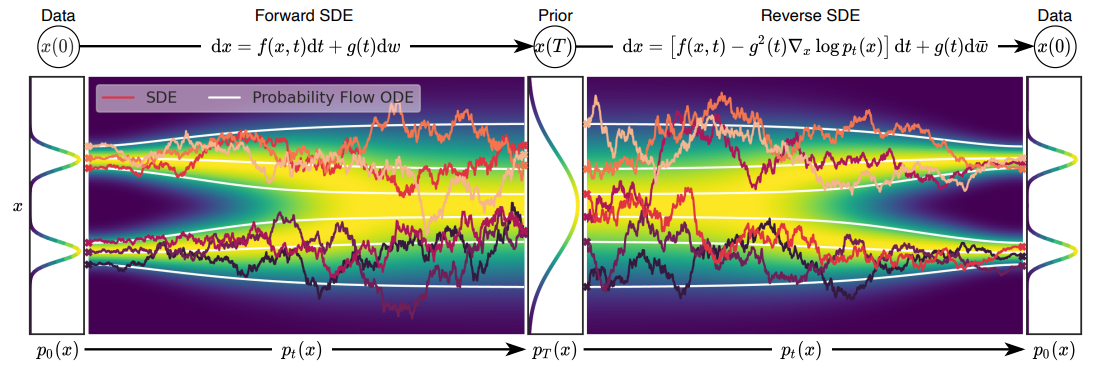
\includegraphics[width=\textwidth]{2.png}
    \caption{\textbf{Tổng quan của một mô hình sinh dựa trên điểm số với phương trình SDE}
    Ta có thể ánh xạ dữ liệu thành một phân phối nhiễu (phân phối tiên nghiệm) với một phương trình SDE (mục \ref{Pertubring-data-with-SDE}) và đảo ngược phương trình SDE này cho quá trình sinh dữ liệu (mục ).
    Ta cũng có thể đảo ngược dòng xác suất tương ứng phương trình ODE (mục ) thu được một quá trình tất định lấy mẫu từ cùng phân phối với SDE.
    Cả phương trình SDE đảo ngược thời gian và dòng xác suất phương trình ODE có thể đạt được bằng các ước lượng điểm số $\nabla_{\bold{x}} \log p_t (\bold{x})$ (mục \ref{Estimating-Scores-For-The-SDE}).}
    \label{fig:2}
\end{figure}

\subsection{Làm xáo trộn dữ liệu với phương trình SDE} \label{Pertubring-data-with-SDE}

Mục đích của ta là xây dựng một quá trình khuếch tán $\lbrace \bold{x}(t) \rbrace_{t=0}^T$ được đánh chỉ số bởi một biến thời gian liên tục $t \in \lbrack 0, T \rbrack$ ví dụ $\bold{x}(0) \sim p_0$, giả sử nếu ta có một bộ dữ liệu mà các điểm dữ liệu là độc lập và cùng phân phối, và $\bold{x}(T) \sim p_T$ là một dạng rất dễ xử lý để sinh các mẫu dữ liệu hiệu quả.
Hay nói cách khác, $p_0$ là phân phối dữ liệu và $p_T$ là phân phối tiên nghiệm.
Quá trình khuếch tán có thể được mô hình hóa là nghiệm của phương trình Ito SDE:

\begin{equation} \label{eq:5}
    d \bold{x} = \bold{f} (\bold{x}, t) dt + g(t) d \bold{w}
\end{equation}

với $\tilde{\bold{w}}$ là một quá trình Wiener chuẩn tắc (hay còn được gọi là chuyển Brown), $\bold{f}(.,t): \mathbb{R}^d \rightarrow \mathbb{R}^d$ là một hàm vector được gọi là hệ số độ trôi của $\bold{x}(t)$ và $g(.): \mathbb{R} \rightarrow \mathbb{R}$ là một hàm vô hướng được gọi là hệ số khuếch tán của $\bold{x}(t)$.
Để cho thuận tiện cho việc trình bày ta giả sử hệ số khuếch tán là một số vô hướng (thay vì là một ma trận $d \times d$) và không phụ thuộc vào $\bold{x}$, nhưng lý thuyết của ta có thể được tổng quát hóa và vẫn đúng trong trường hợp này (phụ lục ).
Phương trình SDE có một nghiệm riêng mạnh chừng nào các hệ số vẫn là Lipschitz toàn cục trong cả trạng thái và thời gian \citep{oksendal2003stochastic}.
Từ sau đây ta ký hiệu $p_t (\bold{x})$ là hàm mật độ xác suất của $\bold{x}(t)$ và sử dụng $p_{st}(\bold{x}(t) \vert \bold{x}(s))$ để ký hiệu nhân chuyển tiếp từ $\bold{x}(s)$ sang $\bold{x}(t)$, với $0 \leq s < s \leq T$.

Thông thường, $p_T$ là một phân phối phi cấu trúc không bao gồm thông tin nào của $p_0$, ví dụ như phân phối Gaussian với trung bình và phương sai cố định.
Có nhiều cách để thiết kế SDE trong phương trình \ref{eq:5} trong quá trình khuếch tán phân phối dữ liệu thành một phân phối tiên nghiệm cố định.
Ta cung cấp một số ví dụ trong mục  thu được quá trình tổng quát hóa liên tục của SMLD và DDPM.

\subsection{Sinh mẫu dữ liệu bằng cách đảo ngược phương trình SDE}

Ta bắt đầu từ các mẫu dữ liệu nhiễu $\bold{x}(T) \sim p_T$ và đảo ngược quá trình, ta có thể thu được các mẫu $\bold{x}(0) \sim p_0$.
Một kết quả đáng chú ý từ \citep{anderson1982reverse} chỉ ra rằng đảo ngược một quá trình khuếch tán cũng là một quá trình khuếch tán, đi ngược theo thời gian bởi một phương trình SDE đảo ngược thời gian:

\begin{equation} \label{eq:6}
    d \bold{x} = \big \lbrack \bold{f}(\bold{x}, t) - g(t)^2 \nabla_{\bold{x}} \log p_t (\bold{x}) \big \rbrack dt + g(t) d \hat{\bold{w}}
\end{equation}

với $\hat{\bold{w}}$ là một quá trình Wiener chuẩn tắc khi thời gian đi ngược từ $T$ về $0$, và $dt$ là một vi phân gia số thời gian âm.
Một khi điểm số của phân phối cận biên $\nabla_{\bold{x}} p_t(\bold{x})$ được biết với mọi $t$, ta có thể thu được quá trình khuếch tán ngược từ phương trình \ref{eq:6} và mô phỏng quá trình này để thu được mẫu dữ liệu từ phân phối $p_0$.

\subsection{Ước lượng điểm số cho phương trình SDE} \label{Estimating-Scores-For-The-SDE}

Điểm số của một phân phối có thể được ước lượng bằng cách huấn luyện một mô hình dựa trên điểm số trên các mẫu với khớp điểm số \citep{hyvarinen2005estimation,song2020sliced}. Để ước lượng $\nabla_{\bold{x}} \log p_t(\bold{x})$, ta có thể huấn luyện một mô hình dựa trên điểm số phụ thuộc vào thời gian $\bold{s}_{\boldsymbol{\theta}}(\bold{x}, t)$ thông qua một tổng quát hóa liên tục từ phương trình \ref{eq:1} và phương trình \ref{eq:3}:

\begin{equation} \label{eq:7}
    \boldsymbol{\theta}^{\ast} = \argmin_{\boldsymbol{\theta}} \mathbb{E}_t \Big \lbrace  \lambda(t) \mathbb{E}_{\bold{x}(0)} \mathbb{E}_{\bold{x}(t) \bold{x}(0)} \big \lbrack \lVert \bold{s}_{\boldsymbol{\theta}} (\bold{x}(t), t) - \nabla_{\bold{x}(t)} \log p_{0t} (\bold{x}(t) \vert \bold{x}(0)) \rVert_2^2 \big \lbrack \Big \rbrace
\end{equation}

với $\lambda: \lbrace 0, T \rbrace \rightarrow \mathbb{R}_{>0}$ là một hàm trọng số dương,
$t$ được lấy mẫu theo phân phối đều trên đoạn $\lbrace 0, T \rbrace$, $\bold{x}(0) \sim p_0 (\bold{x})$ và $\bold{x}(t) \sim p_{0t} (\bold{x}(t) \vert \bold{x}(0))$.
Với mô hình có kích thước và lượng dữ liệu phù hợp, khớp điểm số đảm bảo lời giải tối ưu của phương trình \ref{eq:7} được ký hiệu bởi $\bold{s}_{\boldsymbol{\theta}^{\ast}}(\bold{x}, t)$ bằng với $\nabla_{\bold{x}} \log p_t (\bold{x})$ với hầu hết $\bold{x}$ và $t$.
Trong SMLD và DDPM, ta thường chọn $\lambda \propto 1 / \mathbb{E} \big \lbrack \lVert \nabla_{\bold{x}(t)} \log p_{0t} (\bold{x}(t) \vert \bold{x}(0)) \rVert_2^2 \big \rbrack$.
Ta cần chú ý rằng công thức \ref{eq:7} sử dụng khớp điểm số khử nhiễu nhưng các hàm mục tiêu khớp điểm số khác ví dụ như khớp điểm số theo lát \citep{song2020sliced} và khớp điểm số sai phân hữu hạn \citep{pang2020efficient} cũng có thể được áp dụng ở đây.

Ta thường cũng cần phải biết nhân chuyển tiếp $p_{0t} (\bold{x}(t) \vert \bold{x}(0))$ để giải phương trình \ref{eq:7} một cách hiệu quả.
Nếu $\bold{f}(.,t)$ là hàm affine, nhân chuyển tiếp luôn luôn là phân phối Gaussian mà trung bình và phương sai thường được biết trong dạng đóng và có thể thu được bằng các kỹ thuật chuẩn tắc (xem mục 5.5  trong \cite{sarkka2019applied}).
Với phương trình SDE tổng quát hơn, ta có thể giải phương trình Kolmogorov thuận \citep{oksendal2003stochastic} để thu được $p_{0t} (\bold{x}(t) \vert \bold{x}(0))$.
Một cách khác, ta có thể mô phỏng phương trình SDE để lấy mẫu từ $p_{0t}(\bold{x}(t) \vert \bold{x}(0))$ và thay thế thành phần khớp điểm số khử nhiễu trong \ref{eq:7} với khớp điểm số theo lát để huấn luyện mô hình mà bỏ qua việc tính toán $\nabla_{\bold{x}(t)} \log p_{0t} (\bold{x}(t) \vert \bold{x}(0))$ (xem phụ lục ).

\subsection{Một số ví dụ: VE, VP SDE và các SDE khác}

Nhiễu được dùng để làm xáo trộn dữ liệu trong SMLD và DDPM có thể được xem là phiên bản rời rạc hóa của hai phương trình SDE khác nhau.
Ta sẽ nói ngắn gọn về phần này và chi tiết dudocj trình bày ở phụ lục .

Khi ta sử dụng $N$ mức nhiễu, từng nhân xáo trộn dữ liệu $p_{\sigma_i}(\bold{x} \vert \bold{x}_0)$ của SMLD tương ứng với phân phối của $\bold{x}_i$ theo xích Markov sau:

\begin{equation}
    \bold{x}_i = \bold{x}_{i-1} + \sqrt{\sigma_i^2 - \sigma_{i-1}^2} \bold{z}_{i-1}, i=1, \dots, N
\end{equation}

với $\bold{z}_{i-1} \sim \mathcal{N}(\bold{0}, \bold{I})$ và ta đã đặt $\sigma_0=0$ để làm đơn giản hóa ký hiệu.
Khi $N \rightarrow \infty$, $\lbrace \sigma_i \rbrace_{i=1}^N$ trở thành một hàm $\sigma(t)$, $\bold{z}_i$ trở thành $\bold{z}_t$, và xích Markov $\lbrace \bold{x}_i \rbrace_{i=1}^N$ trở thành một quá trình ngẫu nhiên liên tục $\lbrace \bold{x}(t) \rbrace_{t=0}^1$, ta sử dụng biến thời gian liên tục $t \in \lbrack 0, 1 \rbrack$ để đánh chỉ số thay vì số nguyên $i$.
Quá trình $\lbrace \bold{x}(t) \rbrace_{t=0}^1$ được cho bởi phương trình SDE sau:

\begin{equation} \label{eq:9}
    d \bold{x} = \sqrt{\dfrac{d \lbrack \sigma^2(t) \rbrack}{dt}} d \bold{w}
\end{equation}

Tương tự như với nhân gây xáo trộn $\lbrace p_{\alpha_i} (\bold{x} \vert \bold{x}_0) \rbrace_{i=1}^N$ của DDPM, xích Markov rời rạc là:

\begin{equation} \label{eq:10}
    \bold{x}_i = \sqrt{1 - \beta_i} \bold{x}_{i-1} + \sqrt{\beta_i} \bold{z}_{i-1}, i=1,\dots,N
\end{equation}

Khi $N \rightarrow \infty$, phương trình \ref{eq:10} hội tụ về phương trình SDE sau đây:

\begin{equation} \label{eq:11}
    d \bold{x} = \dfrac{1}{2} \beta(t) \bold{x} dt + \sqrt{\beta(t)} d\bold{w}
\end{equation}

vì vậy, nhiễu dùng để xáo trộn được dùng trong SMLD và DDPM tương ứng với sự rời rạc hóa của phương trình SDE trong công thức \ref{eq:9} và \ref{eq:11}.
Một điều thú vị là phương trình SDE của công thức \ref{eq:9} luôn luôn tạo ra một quá trình với phương sai bùng nổ khi $t \rightarrow \infty$, trong khi phương trình ở công thức \ref{eq:11} thu được một quá trình với phương sai không đổi là một khi phân phối ban đầu có phương sai là một (chứng minh ở phụ lục ).
Vì sự khác biệt này, kể từ đây ta sẽ gọi phương trình ở công thức \ref{eq:9} là Variance Exploding (VE) SDE, và phương trình ở công thức \ref{eq:11} là Variance Preserving (VP) SDE.

Lấy cảm hứng từ VP SDE, ta đề xuất một loại phương trình SDE mới đặc biệt tốt trên độ hợp lý (mục ) được cho bởi công thức:

\begin{equation} \label{eq:12}
    d \bold{x} = -\dfrac{1}{2} \beta(t) \bold{x} dt + \sqrt{\beta(t) (1-e^{-2\int_{0}^{t} \beta(s)ds} )} d \bold{w}
\end{equation}

Khi sử dụng cùng $\beta(t)$ và bắt đầu từ cùng một phân phối ban đầu, phương sai của quá trình ngẫu nhiên thu được từ phương trình \ref{eq:12} luôn luôn bị chặn bởi VPSDE tại mỗi bước thời gian trung gian (chứng minh ở phục lục ).
Vì lý do này, ta đặt tên công thức \ref{eq:12} là sub-VP SDE.

Khi VE, VP, sub-VP SE đều có một độ trôi, nhân làm xáo trộn dữ liệu $p_{0t}(\bold{x}(t) \vert \bold{x}(0))$ tất cả đều có phân phối Gaussian và có thể được tính ở dạng đóng đã được trình bày ở mục \ref{Estimating-Scores-For-The-SDE}.
Điều này làm việc huấn luyện mô hình với công thức \ref{eq:7} đặc biệt hiệu quả.

\section{Giải phương trình SDE ngược}

Sau khi huấn luyện một mô hình dựa trên điểm số phụ thuộc vào thời gian $\bold{s}_{\boldsymbol{\theta}}$, ta có thể sử dụng mô hình này để xây dựng một phương trình SDE đảo ngược thời gian và sau đó mô phỏng nó với cách tiếp cận phuowg pháp số để sinh ra các mẫu dữ liệu từ phân phối $p_0$.

\subsection{Bộ giải phương trình SDE bằng phương pháp số đa chức năng}

\begin{table}[h!]
    \centering
    \caption{So sánh các bộ giải phương trình SDE đảo ngược thời gian khác nhau trên tập CIFAR-10.
    Vùng tối màu thu được với cùng cách tính toán (số các hàm điểm số).
    Trung bình và độ lệch tiêu chuẩn được đưa ra trên 5 lần chạy.
    "P1000" hoặc "P2000": bộ lấy mẫu mà chỉ dự đoán sử dụng 1000 hoặc 2000 bước.
    "C2000": bộ lấy mẫu chỉ căn chỉnh sử dụng 2000 bước.
    "PC1000": Bộ lấy mẫu dự đoán căn chỉnh sử dụng 1000 bước dự đoán và 1000 bước căn chỉnh.}
    \resizebox{\columnwidth}{!}{
        \begin{tabular}{c|c|c|c|c|c|c|c|c}
            \hline
            & \multicolumn{4}{|c|}{Variance Exploding SDE (SMLD)} & \multicolumn{4}{|c}{Variance Preserving SDE (DDPM)} \\
            \hline
            FID $\downarrow$ & P1000 & P2000 & C2000 & PC1000 & P1000 & P2000 & C2000 & PC1000 \\
            \hline
            ancestral sampling & 4.98 $\pm$ .06 & 4.88 $\pm$ .06 & \multirow{3}{*}{20.43 $\pm$ .07} & \textbf{3.62} $\pm$ \textbf{.03} & 3.24 $\pm$  .02 & 3.24 $\pm$ .02 & \multirow{3}{*}{19.06 $\pm$ .06} & \textbf{3.21} $\pm$ \textbf{.02} \\
            reverse diffusion & 4.79 $\pm$ .07 & 4.74 $\pm$ .08 & & \textbf{3.60} $\pm$ \textbf{.02} & 3.21 $\pm$  .02 & 3.19 $\pm$ .02 & & \textbf{3.18} $\pm$ \textbf{.01} \\
            probability flow & 15.41 $\pm$ .15 & 10.54 $\pm$ .08 & & \textbf{3.51} $\pm$ \textbf{.04} & 3.59 $\pm$  .04 & 3.23 $\pm$ .03 & & \textbf{3.06} $\pm$ \textbf{.03} \\
            \hline
        \end{tabular}
    }
    \label{tab:1}
\end{table}

Các bộ giải sử dụng phương pháp số tạo ra một quỹ đạo xấp xỉ từ phương trình SDE.
Tồn tại nhiều phương pháp số đa chức năng để giải phương trình SDE như Euler-Maruyama và phương pháp Runge-Kutta ngẫu nhiên, tương ứng với các cách rời rạc hóa khác nhau của động học ngẫu nhiên.
Ta có thể áp dụng bất kỳ cách nào cho phương trình SDE đảo ngược thời gian để sinh mẫu dữ liệu.

Ancestral sampling, là phương pháp lấy mẫu của DDPM trong công thức \ref{eq:4} thực tế tương ứng với một phương pháp rời rạc hóa đặc biệt của phương trình VP SDE đảo ngược thời gian (công thức \ref{eq:11}) (phụ lục ).
Để thu được luật lấy mẫu sử dụng ancestral sampling cho phương trình SDE mới không phải là việc dễ dàng.
Để khắc phụ điều này, ta đề xuất \textit{bộ lấy mẫu khuếch tán ngược} (chi tiết trong phụ lục ), bộ lấy mẫu này rời rạc hóa phương trình SDE đảo ngược thời gian theo cùng cách với phương trình thuận, và vì vậy có thể đễ dàng thực hiện sử dụng kết quả rời rạc hóa của quá trình thuận
Hình \ref{tab:1}, bộ lấy mẫu khuếch tán ngược thể hiện tốt hơn một chút so với ancestral sampling cho cả hai mô hình SMLD và DDPM trên CIFAR-10 (mô hình DDPM sử dụng ancestral sampling cũng có thể áp dụng cho mô hình SMLD, xem phụ lục ).

\subsection{Bộ lấy mẫu dự đoán - căn chỉnh}

Không giống với phương trình SDE tổng quát, ta có thêm thông tin có thể sử dụng để cải thiện lời giải.
Khi ta có một mô hình dựa trên điểm số $\bold{s}_{\boldsymbol{\theta}^{\ast}} (\bold{x}, t)\approx \nabla_{\bold{x}} \log p_t (\bold{x})$, ta có thể sử dụng cách tiếp cận MCMC dựa trên điểm số ví dụ như Langevin MCMC \citep{parisi1981correlation,grenander1994representations} hoặc HMC \citep{neal2011mcmc} để lấy mẫu trực tiếp từ $p_t$ và căn chỉnh lời giải của một bộ giải phương trình SDE bằng phương pháp số.

Cụ thể, tại từng bước thời gian, bộ giải phương trình SDE bằng phương pháp số ban đầu tạo ra một ước lượng của mẫu tại bước tiếp theo, đóng vai trò là một "bộ dự đoán".
Sau đó, ta dùng MCMC dựa trên điểm số căn chỉnh phân phối cận biên của mẫu đã được ước lượng, đóng vai trò là "bộ căn chỉnh".
Ý tưởng tương tự với phương pháp dự đoán - căn chỉnh, một họ của các kỹ thuật phương pháp số cho giải hệ phương trình \citep{allgower2012numerical} và ta đặt một tên tương tự cho thuật toán lấy mẫu là bộ lấy mẫu \textit{dự đoán - căn chỉnh}.
Mã giả được được trình bày ở phụ lục .
Bộ lấy mẫu PC tổng quát hóa các phương pháp lấy mẫu ban đầu của SMLD và DDPM: các phương pháp trước đây sử dụng một hàm đồng nhất là hàm dự đoán và tôi luyện động học Langevin làm bộ căn chỉnh, trong khi các phương pháp sau sử dụng ancestral sampling là bộ dự đoán và hàm đồng nhất là bộ căn chỉnh.

Ta sẽ thử bộ lấy mẫu PC trên các mô hình SMLD và DDPM (thuật toán và thuật toán trong phụ lục) được huấn luyện với hàm mục tiêu rời rạc ban đầu trong các công thức \ref{eq:1} và \ref{eq:3}.
Các công thức này cho ta thấy sự phù hợp của bộ lấy mẫu PC với mô hình dựa trên điểm số được huấn luyện với một số bước cố định các mức nhiễu.
Ta tổng hợp khả năng của các bộ lấy mẫu khác nhau trong bảng \ref{tab:1}, với dòng xác suất là một bộ dự đoán sẽ được trình bày ở trong mục \ref{Probability-Flow-and-Connection-to-Neural-ODEs}.
Cấu hình chi tiết về các thí nghiệm và các kết quả chi tiết hơn được trình phù ở phụ lục.
Ta quan sát thấy rằng bộ lấy mẫu khuếch tán ngược luôn luôn tốt hơn so với các phương pháp ancestral sampling, chỉ căn chỉnh (C2000) và kém hơn so với các bộ lấy mẫu khác (PC2000, PC1000) cùng với lượng tính toán.
(Thực tế, ta cần nhiều bước căn chỉnh hơn trên một mức nhiễu, và vì vậy cần tính toán nhiều hơn để khớp với khả năng của các bộ lấy mẫu khác)
Với tất cả các bộ dự đoán, thêm một bước căn chỉnh cho từng bước dựa đoán (PC1000) làm tăng khối lượng tính toán lên gấp đôi nhưng luôn luôn cải thiện chất lượng mẫu (so với PC1000).
Hơn nữa, thông thường việc thêm một bước dự đoán và căn chỉnh thường tốt hơn tăng gấp đôi số bước dự đoán mà không thêm bước căn chỉnh (P2000),
khi ta luôn phải nội suy giữa những mức nhiễu (chi tiết trong phụ lục) cho các mô hình SMLD/DDPM.
Trong hình (phụ lục), ta cung cấp thêm so sánh về mặt chất các mô hình cho các hàm mục tiêu trong công thức \ref{eq:7} trên tập LSUN 256 $\times$ 256 và VE SDE, với các bộ lấy mẫu PC vượt trội hơn hẳn các bộ lấy mẫu chỉ dự đoán với cùng một khối lượng tính toán khi ta dùng một số lượng phù hợp các bước căn chỉnh.

\subsection{Dòng xác suất và sự liên kết với các phương trình ODE neuron} \label{Probability-Flow-and-Connection-to-Neural-ODEs}

Các mô hình dựa trên điểm số cho phép phương pháp số khác nhau để giải các phương trình SDE đảo ngược thời gian.
Với tất cả các quá trình khuếch tán, tồn tại một quá trình tất định tương ứng mà quỹ đạo này chia sẻ cùng một hàm mật độ xác suất cận biên $\lbrace p_t (\bold{x}) \rbrace_{t=0}^T$ cùng với phương trình SDE.
Quá trình tất định này thỏa mãn một phương trình ODE (chi tiết được trình bày trong phục lục ):

\begin{equation} \label{eq:13}
    d \bold{x} = \Big \lbrack \bold{f}(\bold{x}, t) - \dfrac{1}{2}g(t)^2 \nabla_{\bold{x}} \log p_t (\bold{x}) \Big \rbrack dt
\end{equation}

có thể được xác định từ một phương trình SDE khi điểm số đã được biết.
Ta đặt tên ODE trong công thức \ref{eq:13} là phương trình ODE dòng xác suất.
Khi hàm điểm số được xấp xỉ bởi một mô hình dựa trên điểm số phụ thuộc vào thời gian, thường là một mạng neuron là một ví dụ của một ODE neuron \citep{chen2018neural}.

\textbf{Tính toán chính xác độ hợp lý} Tận dụng sự liên kết với các phương trình ODE neuron, ta có thể tính hàm mật độ được định nghĩa bởi công thức \ref{eq:13} thông qua sự thay đổi tức thời của các biến trong công thức \citep{chen2018neural}.
Điều này cho phép ta tính toán được \textit{chính xác độ hợp lý trên bất kỳ dữ liệu đầu vào nào} (chi tiết trong phụ lục).
Một ví dụ, ta báo cáo hàm âm log của độ hợp lý (negative log-likelihoods - NLLs) được đo trên bits/dim trên tập CIFAR-10 trong bảng \ref{tab:2}.
Ta tính log của độ hợp lý một cách đồng đều trên dữ liệu đã được giải lượng tự và chỉ so sánh với có các mô hình được đánh giá theo cùng một cách (bỏ qua các mô hình được đánh giá với giải lượng tử hóa biến phân \citep{ho2019flow++} hoặc ữ liệu rời rạc), ngoại trừ với DDPM (L/$L_{\mathrm{simple}}$) mà giá trị ELBO (được gán nhãn với $\ast$) được báo cáo trên tập rời rạc.
Các kết quả chính: (i) Với cùng mô hình DDPM trong \citep{ho2020denoising}, ta thu được bits/dim cao hơn ELBO, khi độ hợp lý của ta là chính xác;
(ii) Sử dụng cùng cấu trúc, ta huấn luyện mô hình DDPM khác với hàm mục tiêu liên tục trong công thức \ref{eq:7} cũng cải thiện thêm độ hợp lý;
(iii) với sub-VP SDEs, ta luôn luôn thu được độ hợp lý cao hơn so với VP SDEs;
(iv) với kiến trúc được cải thiện (ví dụ DDPM++ ở mục ) và sub-VP SDE, ta có thể lập một kỷ lục mới bits/dim là 2.99 trên tập CIFAR-10 giải lượng tử đều ngay cả không sử dụng \textit{huấn luyện cực đại hóa độ hợp lý}.


\begin{table}[h!]
    \centering
    \caption{NLLs và FIDs (ODE) trên tập CIFAR-10}
    \begin{tabular}{lcc}
        \hline
        Model & NLL Test $\downarrow$ & FID $\downarrow$ \\
        \hline
        RealNVP \citep{dinh2016density} & 3.49 & - \\
        iResNet \citep{behrmann2019invertible} & 3.45 & - \\
        Glow \citep{kingma2018glow} & 3.35 & - \\
        MintNet \citep{song2019mintnet} & 3.32 & - \\
        Residual Flow \citep{chen2019residual} & 3.28 & 46.37 \\
        FFJORD \citep{grathwohl2018ffjord} & 3.40 & - \\
        Flow++ \citep{ho2019flow++} & 3.29 & - \\
        DDPM (L) \cite{ho2020denoising} & $\leq 3.70^{\ast}$  & 13.51 \\
        DDPM ($L_{\mathrm{simple}}$) \citep{ho2020denoising} & $\leq 3.75^{\ast}$ & 3.17 \\
        \hline
        DDPM & 3.28 & 3.37 \\
        DDPM cont. (VP) & 3.21 & 3.69 \\
        DDPM cont. (sub-VP) & 3.05 & 3.56 \\
        DDPM++ cont. (VP) & 3.16 & 3.93 \\
        DDPM++ cont. (sub-VP) & 3.02 & 3.16 \\
        DDPM++ cont. (deep, VP) & 3.13 & 3.08 \\
        DDPM++ cont. (deep, sub-VP) & \textbf{2.99} & \textbf{2.92} \\
        \hline
    \end{tabular}
    \label{tab:2}
\end{table}

\begin{table}[h!]
    \centering
    \caption{Chất lượng các mẫu trên tập CIFAR-10}
    \begin{tabular}{lcc}
        \hline
        Model & FID $\downarrow$ & IS $\uparrow$ \\
        \hline
        \textbf{Conditional} & & \\
        BigGAN \citep{brock2018large} &  14.73 & 9.22 \\
        StyleGAN2-ADA \citep{karras2020training} & \textbf{2.42} & \textbf{10.14} \\
        \hline
        \textbf{Unconditional} & & \\
        StyleGAN2-ADA \citep{karras2020training} & 2.92 & 9.83 \\
        NCNS \citep{song2019generative} & 25.32 & 8.87 $\pm$ .12 \\
        NCNSv2 \citep{song2020improved} & 10.87 & 8.40 $\pm$ .07 \\
        DDPM \citep{ho2020denoising} & 3.17 & 9.46 $\pm$ .11 \\
        \hline
        DDPM++ & 2.78 & 9.64 \\
        DDPM++ cont. (VP) & 2.55 & 9.58 \\
        DDPM++ cont. (sub-VP) & 2.61 & 9.56 \\
        DDPM++ cont. (deep, VP) & 2.41 & 9.68 \\
        DDPM++ cont. (deep, sub-VP) & 2.41 & 9.57 \\
        NCSN++ & 2.45 & 9.73 \\
        NCSN++ cont. (VE) & 2.38 & 9.83 \\
        NCSN++ cont. (deep, VE) & \textbf{2.20} & \textbf{9.89} \\
        \hline
    \end{tabular}
    \label{tab:3}
\end{table}

\textbf{Thao tác trên biểu diễn ẩn} Bằng cách kết hợp công thức \ref{eq:13}, ta có thể mã hóa bất kỳ điểm dữ liệu $\bold{x}(0)$ nào vào một không gian ẩn $\bold{x}(T)$.
Giải mã có thể thu được bằng cách kết hợp phương trình ODE tương ứng cho phương trình SDE đảo ngược thời gian.
Như đã được thực hiện với các mô hình có thể đảo ngược khác như ODEs neuron và dòng chuẩn hóa \citep{dinh2016density, kingma2018glow}, ta có thể thao tác biểu diễn này cho chỉnh sửa ảnh, như nội suy và chia tỷ lệ nhiệt độ.

\textbf{Mã hóa có thể nhận dạng duy nhất} Không giống như hầu hết các mô hình có thể đảo ngược hiện tại,
cách mã hóa của ta là có thể nhận diện duy nhất, nghĩa là với dữ liệu huấn luyện phù hợp, kích thước mô hình và độ chính xác tối ưu, mã hóa cho một input được xác định duy nhất bởi phân phối dữ liệu \citep{roeder2021linear}.
Bởi vì phương trình SDE thuận, công thức \ref{eq:5} không có tham số huấn luyện được, và tương ứng với dòng xác suất ODE, công thức \ref{eq:13} cho ta cùng quỹ đạo khi cho ước lượng điểm số hoàn hảo.
Ta cung cấp các kiểm chứng thực nghiệm bổ sung về tính chất này ở phục lục .

\begin{figure}[h!]
    \centering
    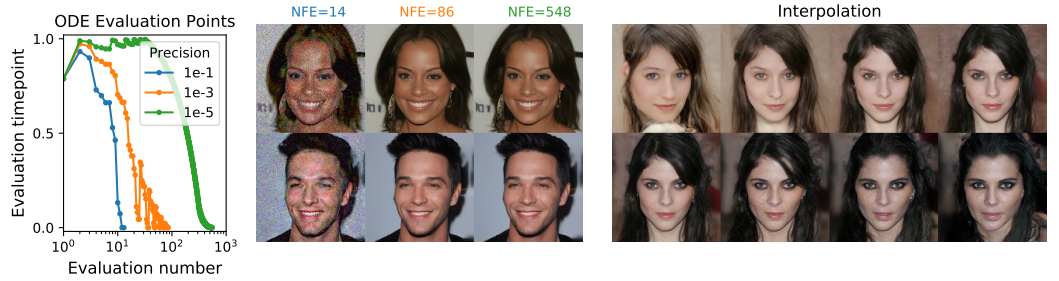
\includegraphics[width=0.9\linewidth]{figures/3.png}
    \caption{\textbf{ODE dòng xác suất cho phép lấy mẫu nhanh} với độ dài bước thích nghi và độ chính xác số học thích nghi thay đổi (\textit{hình trái}), giảm số lần đánh giá hàm điểm số (NFE) mà không làm ảnh hưởng đến chất lượng (\textit{hình giữa}).
    Ánh xạ ngược từ không gian ẩn sang ảnh cho phép nội suy (\textit{hình phải})}
    \label{fig:3}
\end{figure}

\textbf{Lấy mẫu hiệu quả} Với một ODE neuron, ta có thể lấy mẫu $\bold{x}(0) \sim p_0$ bằng cách giải phương trình ở công thức \ref{eq:13} từ các điều kiện $\bold{x}(T) \sim p_T$.
Sử dụng một chiến lược rời rạc hóa cố định ta có thể tạo ra các mẫu có khả năng cạnh tranh cao, đặc biệt khi sử dụng cùng vơi shbooj hiệu chỉnh (bảng \ref{tab:1}, "bộ lấy mẫu dòng xác suất", chi tiết ở phụ lục).
Sử dụng một bộ giải phương trình ODE dạng hộp đen \citep{dormand1980family} không những chỉ tạo ra những mẫu chất lượng cao (\ref{tab:2}, chi tiết ở phụ lục ) mà còn cho phép ta đánh đổi độ chính xác cho tính hiệu quả.
Với khả năng chống chịu sai lệch cao hơn, số hàm đánh giá có thể được giảm hơn 90 \% mà không cần làm ảnh hưởng chất lượng của mẫu (hình \ref{fig:3})

\subsection{Các cải thiện về kiến trúc của mô hình}

Ta khám phá nhiều thiết kế kiến trúc mới cho mô hình dựa trên điểm số sử dụng cả VE và VP SDEs (chi tiết ở phụ lục ), với ta huấn luyện các mô hình với các hàm mục tiêu rời rạc như SMLD/DDPM.
Ta áp dụng trực tiếp các kiến trúc của VP SDEs cho sub-VP SDEs vì tính tương đồng của hai mô hình này.
Kiến trúc tối ưu ta thấy cho VE SDE được gọi là NCSN++ thu được FID là 2.45 trên CIFAR-10, với bộ lấy mẫu PC, trong khi kiến trúc tối ưu cho VP SDE được gọi là DDPM++ đạt được kết quả với FID là 2.78.

Bằng cách chuyển sang sử dụng công thức huấn luyện liên tục ở công thức \ref{eq:7} và tăng độ sâu của mạng, ta có thể cải thiện hơn nữa chất lượng của mẫu cho tất cả các mô hình.
Các kiến trúc được chọn được ký hiệu là NCSN++ cont. và DDPM++ cont. trong bảng \ref{tab:3} lần lượt cho VE và VP/sub-VP SDEs.
Các kết quả được báo cáo trong bảng \ref{tab:3} tương ướng với các checkpoint với FID nhỏ nhất trong quá trình huấn luyện, với các mẫu được tạo ra với bộ lấy mẫu PC.
Ngược lại, chỉ số FID và các giá trị NLL trong bảng \ref{tab:2} được báo cáo cho checkpoint cuối cùng trong quá trình huấn luyện, và các bộ lấy mẫu thu được với một bộ giải phương trình ODE là một hộp đen.
Như được trình bày trong b ảng \ref{tab:3}, VE SDEs thường cho các mẫu có chất lượng tốt hơn VP/sub-VP SDE.
Điều này cho thấy những người người làm thực tiễn có xu hướng thích làm thí nghiệm với các phương trình ngẫu nhiên SDEs khác nhau cho nhiều phạm vi dữ liệu và kiến trúc.

Mô hình cho mẫu chất lượng tốt nhất là NCSN++ cont. (deep, VE), có chiều sâu gấp đôi và tạo kỷ lục mới cho cả inception score và FID cho bài toán sinh mẫu không có điều kiện trên tập CIFAR-10.
Điều khá ngạc nhiên là ta có thể đạt được FID tốt hơn các mô hình sinh có điều kiện tốt nhất trước đây mà không cần dữ liệu được gán nhãn.
Kết hợp tất cả các cải tiến lại, ta cũng thu được tập mẫu với độ chân thực cao trên tập CelebA-HQ 1024 $\times$ 1024 từ các mô hình dựa trên dựa trên điểm số (phụ lục ).
Mô hình tốt nhất của ta cho độ hợp lý là DDPM++ cont. (deep, sub VP), cũng chiều sâu gấp đôi và thu được log của độ hợp lý là 2.99 bits/dim với hàm mục tiêu liên tục trong công thức \ref{eq:7}.
Với những gì ta biết, đây là độ hợp lý cao nhất trên tập CIFAR-10 được lấy mẫu đều.

\section{Sinh mẫu có điều khiển}

Cấu trúc liên tục của khung làm việc của ta cho phép ta không chỉ sinh ra các mẫu dữ liệu từ phân phối $p_0$ mà còn từ phân phối $p_0 (\bold{x}(0) \vert \bold{y})$ nếu $p_t (\bold{y} \vert \bold{x}(t))$ biết.
Khi được cho trước một phương trình SDE thuận trong công thức \ref{eq:5}, ta có thể lấy mẫu từ $p_t(\bold{x}(t) \vert \bold{y})$ bằng cách bắt đầu từ $p_T (\bold{x}(T) \vert \bold{y})$ và giải phương trình SDE đảo ngược thời gian có điều kiện:

\begin{equation} \label{eq:14}
    d \bold{x} = \lbrace \bold{f}(\bold{x}, t) - g (t)^2 \lbrack \nabla_{\bold{x}} \log p_t(\bold{x}) + \nabla_{\bold{x}} \log p_t (\bold{y} \vert \bold{x}) \rbrack \rbrace dt + g(t) d \bar{\bold{w}}
\end{equation}

Tổng quát, ta có thể sử dụng công thức \ref{eq:14} để giải một lớp lớn các \textit{bài toán ngược} với mô hình sinh dựa trên điểm số,
một khi được biết một ước lượng của gradient của quá trình thuận $\nabla_{\bold{x}} \log p_t (\bold{y} \vert \bold{x}(t))$.
Trong một số trường hợp, ta có thể huấn luyện một mô hình riêng biệt để học quá trình thuận $p_t(\bold{y} \vert \bold{x}(t))$ và tính gradient của quá trình này.
Mặt khác, ta có thể ước lượng gradient với kinh nghiệm và kiến thức chuyên gia về một miền dữ liệu.
Ở phụ lục , ta cung cấp các phương pháp được ứng dụng rộng rãi để thu được những ước lượng mà không cần huấn luyện mô hình phụ.

\begin{figure}[h!]
    \centering
    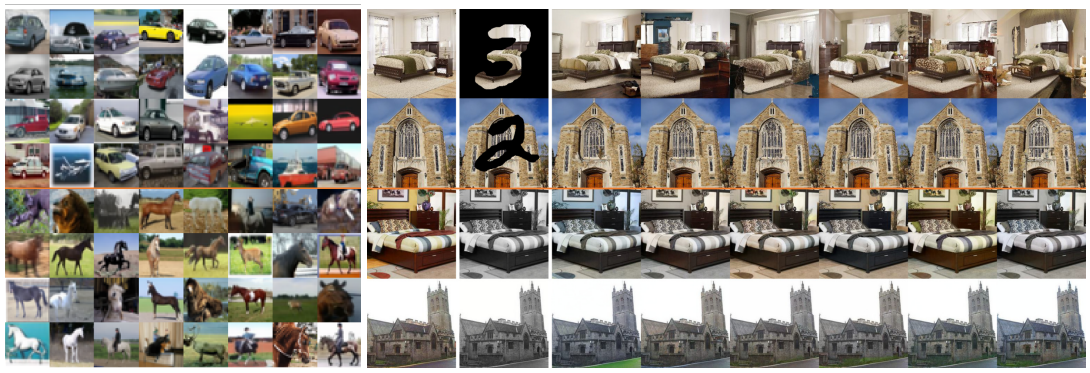
\includegraphics[width=0.9\linewidth]{figures/4.png}
    \caption{\textit{Hình trái:} Các mẫu được tạo ra dựa trên điều kiện về lớp trên tập CIFAR-10 32 $\times$ 32.
    Bốn hàng đầu tiên là oto và bốn hàng cuối là ngựa.
    \textit{Hình phải:} Bài toán inpainting (hai hàng đầu) và bài toán tô màu (hai hàng cuối) kết quả trên tập LSUN 256 $\times$ 256.
    Cột đầu tiên là ảnh gốc, cột thứ hai là ảnh bị gán mặt nạ hoặc chuyển sang ảnh xám, các cột còn lại là các mẫu ảnh được hoàn thiện hoặc được tô màu.}
    \label{fig:4}
\end{figure}

Ta xét ba ứng dụng của bài toán sinh mẫu có điều khiển với các cách tiếp cận:
sinh mẫu có điều kiện dựa trên lớp, xóa một phần ảnh và tô màu.
Khi $\bold{y}$ biểu diễn nhãn lớp, ta có thể huấn luyện một bộ phân loại phụ thuộc vào thời gian $p_t(\bold{y} \vert \bold{x}(t))$ cho bài toán lấy mẫu điều kiện trên lớp.
Khi phương trình thuận SDE dễ giải, ta có thể dễ dàng tạo ra dữ liệu huấn luyện $(\bold{x}(t), \bold{y})$ cho bộ phân loại phụ thuộc vào thời gian bởi lấy mẫu ban đầu $\bold{x}(0), \bold{y}$ từ tập dữ liệu và sau đó lấy mẫu $\bold{x}(t) \sim p_{0t} (\bold{x}(t) \vert \bold{x}(0))$.
Sau đó, ta có thể sử dụng một sự kết ợp của các hàm mất mát cross-entropy trên các bước thời gian khác nhau, như công thức \ref{eq:7}, để huấn luyện bộ phân loại phụ thuộc theo thời gian $p_t(\bold{y} \vert \bold{x}(t))$.
Ta cung cấp các mẫu được sinh ra có điều kiện dựa trên lớp trên tập CIFAR-10 ở hình \ref{fig:4} (hình trái) và các thông tin chi tiết hơn về kết quả ở phụ lục .

Xóa một phần thông tin ảnh là một trường hợp đặc biệt của lấy mẫu có điều kiện.
Giả sử ta có một điểm dữ liệu không hoàn chỉnh $\bold{y}$ với chỉ một tập con, $\Omega(\bold{y})$ biết trước.
Lượng dữ liệu bị xóa từ ảnh để lấy mẫu từ $p(\bold{x}(0) \vert \Omega(\bold{y}))$, ta có thể thực hiện sử dụng một mô hình sinh không có điều kiện (xem phụ lục ).
Bài toán tô màu là một trường hợp đặc biệt của xóa một phần thông tin ảnh, ngoại trừ chiều dữ liệu đã biết.
Ta có thể chiều dữ liệu với một phép biến đổi tuyến tính trực giao và thực hiện xóa thông tin ảnh trong không gian đã bị biến đổi (chi tiết ở trong phụ lục ).
Hình \ref{fig:4} (bên phải) cho biết kết quả cho bài toán xóa thông tin ảnh và tô màu thu được với mô hình dựa trên điểm số phụ thuộc vào thời gian không có điều kiện.

\section{Kết luận}

Ta đã trình bày một khung làm việc cho các mô hình sinh dựa trên điểm số trên các phương trình vi phân ngẫu nhiên SDEs.
Công trình của ta cho phép việc hiểu sâu hơn của các cách tiếp cận đã tồn tại, các thuật toán lấy mẫu mới, tính chính xác độ hợp lý, mã hóa có thể nhận dạng duy nhất, thao tác trên không gian ẩn và mang lại khả năng sinh dữ liệu của mô hình sinh dựa trên điểm số.

Trong khi đó phương pháp tiếp cận ta đề xuất cải thiện các kết quả và cho phép lấy mẫu hiệu quả hơn, nhưng tốc độ lấy mẫu vẫn chậm hơn GANs \citep{goodfellow2020generative} trên cùng các tập dữ liệu.
Nhận biết các cách kết hợp quá trình huấn luyện ổn định của các mô hình sinh dựa trên điểm số kết hợp với lấy mẫu nhanh của các mô hình ngầm định như GANs vẫn là một hướng nghiên cứu quan trọng.
Hơn nữa, độ rộng của bộ lấy mẫu có thể sử dụng khi biết số siêu tham số của hàm điểm số.
các công trình trong tương lai có thể tận dụng từ các phương pháp đã được cải thiện để tự động lựa chọn và tinh chỉnh các siêu tham số cũng như các khám phá mở rộng dựa trên những giá trị và những hạn chế của nhiều phương pháp lấy mẫu khác nhau.
\newpage
\bibliography{iclr2021_conference}
\bibliographystyle{iclr2021_conference}

\newpage

\appendix

Ta trình bày một số phụ lục với các chi tiết bổ sung, chứng minh công thức và kết quả.
Khung làm việc của ta cho phép phương trình SDE tổng quan với các hệ số khuếch tán có giá trị dạng ma trận phụ thuộc vào trạng thái, trong đó ta cung cấp một số nhận xét chi tiết trong phụ lục .
Ta cung cấp chứng minh chi tiết của VE, VP, và sub-VP SDEs trong phụ lục , và ta thảo luận cách sử dụng từ quan điểm thực tiễn ở phụ lục .
Ta xây dựng công thức dòng xác suất trong phụ lục , bao gồm chứng minh thu được công thức dòng xác suất của phương trình ODE (phụ lục ), tính toán chính xác độ hợp lý (phụ lục ), lấy mẫu dòng xác suất với chiến lược rời rạc hóa cố định (phụ lục ),
lấy mẫu bằng bộ giải phương trinh ODE là một hộp đen (phụ lục ), và xác minh các thử nghiệm trên mã hóa có thể nhận dạng duy nhất (phụ lục ).
Ta cung cấp mô tả đầy đủ về bộ lấy mẫu quá trình khuếch tán ngược trong phụ lục ,
bộ lấy mẫu ancestral loại DDPM cho mô hình SMLD trong phụ lục , và bộ lấy mẫu dự đoán - hiệu chỉnh trong phụ lục .
Ta giải thích các kiến trúc của mô hình và các cài đặt thử nghiệm chi tiết trong phụ lục ,
với các mẫu độ phân giải 1024 $\times$ 1024 trên tập CelebA-HQ.
Cuối cùng, ta trình bày chi tiết về các thuật toán sinh mẫu có điều khiển trong phụ lục  và bao gồm các kết quả mở rộng cho sinh dữ liệu dựa trên lớp (phụ lục ),
bài toán tô màu (phụ lục ) và chiến lực cho giải bài toán ngược tổng quát (phụ lục ).

\section{Khung làm việc cho phương trình SDE tổng quát} \label{A}

Trong phần nội dung chính, ta đã giới thiệu khung làm việc dựa trên phương trình SDE ở công thức \ref{eq:5} với hệ số khuếch tán độc với $\bold{x}(t)$.
Cho thấy rằng khung làm việc của ta có thể mở rộng với những tham số khuếch tán tổng quát hơn.
Ta có thể xem xét phương trình SDEs với dạng sau:

\begin{equation} \label{eq:15}
    d \bold{x} = \bold{f} (\bold{x}, t) dt + \bold{G} (\bold{x}, t) d\bold{w}
\end{equation}

với $\bold{f}(., t): \mathbb{R}^d \rightarrow \mathbb{R}^d$ và $\bold{G}(., t): \mathbb{R}^d \rightarrow \mathbb{R}^{d \times d}$.
Ta sử dụng giải thích Ito về SDEs xuyên suốt công trình này.

Theo \citep{anderson1982reverse}, phương trình SDE đảo ngược thời gian được cho bởi công thức (công thức \ref{eq:6}):

\begin{equation} \label{eq:16}
    d \bold{x} = \lbrace \bold{f}(\bold{x}, t) - \nabla . \lbrack \bold{G}(\bold{x}, t) \bold{G}(\bold{x}, t)^T \rbrack - \bold{G}(\bold{x}, t) \bold{G}(\bold{x}, t)^T \nabla_{\bold{x}} \log p_t(\bold{x}) \rbrace dt + \bold{G}(\bold{x}, t) d\bar{\bold{w}}
\end{equation}

với ta định nghĩa $\nabla . \bold{F}(\bold{x}) := (\nabla. \bold{f}^1 (\bold{x}), \nabla. \bold{f}^2 (\bold{x}), \dots, \nabla. \bold{f}^d (\bold{x}))^T$ cho hàm giá trị ma trận $\bold{F}(\bold{x}) := (\bold{f}^1 (\bold{x}), \bold{f}^2 (\bold{x}), \dots, \bold{f}^d (\bold{x}))^T$ xuyên suốt công trình.

Dòng xác suất phương trình ODE tương ứng với công thức \ref{eq:15} có dạng sau (công thức \ref{eq:13}, chứng minh ở phụ lục ):

\begin{equation} \label{eq:17}
    d \bold{x} = \Big \lbrace \bold{f}(\bold{x}, t) - \dfrac{1}{2} \nabla . \lbrack \bold{G}(\bold{x}, t) \bold{G}(\bold{x}, t)^T  \rbrack - \bold{G}(\bold{x}, t) \bold{G}(\bold{x}, t)^T \nabla_{x} \log p_t(\bold{x}) \Big \rbrace dt
\end{equation}

Cuối cùng, cho sinh mẫu có điều kiện với phương trình SDE tổng quát \ref{eq:15}, ta có thể giải phương trình SDE đảo ngược thời gian có điều kiện dưới đây (công thức \ref{eq:14}, chi tiết ở phục lục ):\

\begin{equation} \label{eq:18}
    \begin{aligned}
        d \bold{x} = \Big \lbrace \bold{f}(\bold{x}, t) - \dfrac{1}{2} \nabla . \lbrack \bold{G}(\bold{x}, t) \bold{G}(\bold{x}, t)^T  \rbrack &- \bold{G}(\bold{x}, t) \bold{G}(\bold{x}, t)^T \nabla_{x} \log p_t(\bold{x}) \\
        & -\bold{G}(\bold{x}, t) \bold{G}(\bold{x}, t)^T \nabla_{x} \log p_t(\bold{y} \vert \bold{x})  \Big \rbrace dt + \bold{G}(\bold{x}, t) d \bar{\bold{w}}
    \end{aligned}
\end{equation}

Khi độ trôi và tham số phân tán của một phương trình SDE là không affine, có thể rất khó để tính nhân chuyển tiếp $p_{0t}(\bold{x}(t) \vert \bold{x}(0))$ ở dạng đóng.
Điều này gây trở ngại quá trình huấn luyện của các mô hình dựa trên điểm số, vì công thức \ref{eq:7} cần biết $\nabla_{\bold{x}(t)} \log p_{0t} (\bold{x}(t) \vert \bold{x}(0))$.
Để vượt qua khó khăn này, ta cần thay thế hàm khớp điểm số khử nhiễu trong công thức \ref{eq:7} với các biến thể hiệu quả khác của hàm khớp điểm số không cần tính $\nabla_{\bold{x}(t)} \log p_{0t} (\bold{x}(t) \vert \bold{x}(0))$.
Ví dụ, khi sử dụng hàm khớp điểm số theo lát \citep{song2020sliced}, hàm mục tiêu huấn luyến luyện của ta trong công thức \ref{eq:7} trở thành:


\begin{equation} \label{eq:19}
    \bold{\theta}^{\ast} = \argmin_{\bold{\theta}} \mathbb{E}_t \Bigg \lbrace \lambda (t) \mathbb{E}_{\bold{x}(0)} \mathbb{E}_{\bold{x}(t)} \mathbb{E}_{\bold{v} \sim p_{\bold{v}}} \Bigg \lbrack \dfrac{1}{2} \lVert \bold{s}_{\bold{\theta}} (\bold{x}(t), t) \rVert_2^2 + \bold{v}^T \bold{s}_{\bold{\theta}} (\bold{x}(t), t) \bold{v} \Bigg \rbrack \Bigg \rbrace
\end{equation}

với $\lambda: \lbrack 0, T \rbrack \rightarrow \mathbb{R}^{+}$ là một hàm trọng số dương, $t \sim \mathcal{U}(0, T), \mathbb{E} \lbrack \bold{v} \rbrack = \bold{0}$
Ta có thể luôn luôn mô phỏng SDE để lấy mẫu từ $p_{0t}(\bold{x}(t) \vert \bold{x}(0))$, và giải phương trình ở công thức \ref{eq:19} để huấn luyện mô hình dựa trên điểm số phụ thuộc vào thời gian $\bold{x}_{\bold{theta}}(\bold{x}, t)$.

\section{VE, VP và sub-VP SDEs} \label{B}

Tiếp theo ta cung cấp các dẫn xuất công thức để chỉ ra dùng nhiễu xáo trộn của các mô hình SMLD và DDPM là phiên bản rời rạc hóa của Variance Exploding (VE) và Variance Preserving (VP) SDE tương ứng.
Ta cũng giới thiệu thêm sub-VP SDEs, một phiên bản sửa đổi của VP SDEs thường thu được kết quả tốt hơn ở cả chất lượng mẫu và độ hợp lý.

Đầu tiên, ta sử dụng tổng cộng N ngưỡng nhiễu, từng nhân xáo trộn $p_{\sigma_i} (\bold{x} \vert \bold{x}_0)$ của mô hình SMLD có thể thu được từ xích Markov:

\begin{equation} \label{eq:20}
    \bold{x}_i = \bold{x}_{i-1} + \sqrt{\sigma_i^2 - \sigma_{i-1}^2} \bold{z}_{i-1}, i = 1, \dots, N
\end{equation}

với $\bold{z}_{i-1} \sim \mathcal{N}(\bold{0}, \bold{I}), \bold{x}_0 \sim p_{\mathrm{data}}$ và ta đặt $\sigma_0 = 0$ để đơn giản hóa ký hiệu.
Trong giới hạn $N \rightarrow \infty$, xích Markov $\lbrace \bold{x}_i \rbrace_{i=1}^N$ trở thành một quá trình ngẫu nhiên liên tục $\lbrace \bold{x}(t) \rbrace_{t=0}^1$,
$\lbrace \sigma_i \rbrace_{i=1}^N$ trở thành một hàm $\sigma(t)$ và $\bold{z}_i$ trở thành $\bold{z}(t)$, ta sử dụng biến thời gian liên tục $t \in \lbrack 0, 1 \rbrack$ dành cho chỉ số thay vì số nguyên $i \in \lbrace 1, 2, \dots, N \rbrace$.
Đặt $\bold{x} \big ( \dfrac{i}{N} \big)=\bold{x}_i, \sigma \big( \dfrac{i}{N} \big) = \sigma_i$,
và $\bold{z} \big ( \dfrac{i}{N} \big)=\bold{z}_i$ với $i = 1, 2, \dots, N$.
Ta có thể viết lại công thức \ref{eq:20} với $\Delta t = \dfrac{1}{N}$ và $t \in \lbrace 0, \dfrac{1}{N}, \dots, \dfrac{N-1}{N} \rbrace$:

\begin{equation*}
    \bold{x}(t + \Delta t) = \bold{x}(t) + \sqrt{\sigma^2 (t + \Delta t) - \sigma^2 (t)} \bold{z}(t) \approx \bold{x} (t) + \sqrt{\dfrac{d \lbrack \sigma^2 (t) \rbrack}{dt}\Delta t} \bold{z}(t)
\end{equation*}

với đẳng thức xấp xỉ đúng với $\Delta t \ll 1$.
Trong giới hạn $\Delta t \rightarrow 0$, đẳng thức này tiến đến:

\begin{equation} \label{eq:21}
    d \bold{x} = \sqrt{\dfrac{d \lbrack \sigma^2(t) \rbrack}{dt}} d \bold{w}
\end{equation}

là phương trình VE SDE

Cho nhân xáo trộn $\lbrace p_{\alpha_i} (\bold{x} \vert \bold{x}_0) \rbrace_{i=1}^N$ được sử dụng trong DDPM, xích Markov rời rạc là:

\begin{equation} \label{eq:22}
    \bold{x}_i = \sqrt{1 - \beta_i} \bold{x}_{i-1} + \sqrt{\beta_i} \bold{z}_{i-1}, i = 1, \dots, N
\end{equation}

với $\bold{z}_{i-1} \sim \mathcal{N}(\bold{0}, \bold{I})$.
Để thu được giới hạn của xích Markov này khi $N \rightarrow \infty$, ta định nghĩa một tập phụ trợ các mức nhiễu $\lbrace \bar{\beta}_i = N \beta_i \rbrace_{i=1}^N$ và viết lại phương trình \ref{eq:22} như dưới đây:

\begin{equation} \label{eq:23}
    \bold{x}_i = \sqrt{1 - \dfrac{\bar{\beta}_i}{N}} \bold{x}_{i-1} + \sqrt{\dfrac{\bar{\beta}_i}{N}} \bold{z}_{i-1}, i = 1, \dots, N
\end{equation}

Trong giới hạn $N \rightarrow \infty, \lbrace \bar{\beta}_i \rbrace_{i=1}^N$ trở thành hàm $\beta(t)$ được đánh chỉ số bởi $t \in \lbrack 0, 1 \rbrack$.
Đặt $\beta \big ( \dfrac{i}{N} \big) = \bar{\beta}_i$,
$\bold{x}\big( \dfrac{i}{N} \big) = \bold{x}_i, \bold{z}\big( \dfrac{i}{N} \big) = \bold{z}_i$.
Ta có thể viết xích Markov ở công thức \ref{eq:23} thành như sau với $\Delta t = \dfrac{1}{N}$ và $t \in \lbrace 0, 1, \dots, \dfrac{N-1}{N} \rbrace$:

\begin{equation} \label{eq:24}
    \begin{aligned}
        \bold{x}(t + \Delta t) &= \sqrt{1 - \beta(t + \Delta t) \Delta t} \bold{x}(t) + \sqrt{\beta(t + \Delta t) \Delta t} \bold{z}(t) \\
        &\approx \bold{x}(t) - \dfrac{1}{2}\beta(t + \Delta t) \Delta t \bold{x} (t) + \sqrt{\beta(t + \Delta t) \Delta t} \bold{z} (t) \\
        &\approx \bold{x}(t) - \dfrac{1}{2} \beta(t) \Delta t \bold{x} (t) + \sqrt{\beta(t) \Delta t} \bold{z} (t)
    \end{aligned}
\end{equation}

với đẳng thức xấp xỉ đúng khi $\Delta t \ll 1$.
Vì vậy, trong giới hạn $\Delta t \rightarrow$, công thức \ref{eq:24} hội tụ về phương trình VP SDE có dạng sau:

\begin{equation} \label{eq:25}
    d \bold{x} = - \dfrac{1}{2} \beta(t) \bold{x} dt + \sqrt{\beta(t)} d \bold{w}
\end{equation}

Tới đây, ta đã chỉ ra được là nhiễu làm xáo trộn được sử dụng trong mô hình SMLD và DDPM tương ứng với rời rạc hóa của VE và VP SDEs.
Với VE SDE luôn luôn thu được một quá trình với phương sai bùng nổ khi $t \rightarrow \infty$.
Ngược lại, với VP SDE ta luôn thu được một quá trình với phương sai bị chặn.
Hơn nữa, quá trình có phương sai đơn vị và là hằng số với mọi $t \in \brack 0;\infty $ khi $p(\bold{x}(0))$ có phương sai đơn vị.
Khi VP SDE có độ trôi và các hệ số khuếch tán là affine, ta có thể sử dụng công thức 5.51 trong \citep{sarkka2019applied} để thu được phương trình ODE chi phối sự phá triển của phương sai:

\begin{equation*}
    \dfrac{d \Sigma_{\mathrm{VP}}(t)}{dt} = \beta(t) (\bold{I} - \Sigma_{\mathrm{VP}}(t))
\end{equation*}

với $\Sigma_{\mathrm{VP}}(t) := \Cov \lbrack \bold{x}(t) \rbrack$ với $\lbrace \bold{x}(t) \rbrace_{t=0}^1$ thỏa mãn một phương trình VP SDE.
Giải phương trình ODE này, ta thu được:

\begin{equation} \label{eq:26}
    \Sigma_{\mathrm{VP}}(t) = \bold{I} + e^{\int_{0}^t - \beta(s)ds} (\Sigma_{\mathrm{VP}}(t) - \bold{I})
\end{equation}

Ta nhận thấy rất rõ ràng rằng $\Sigma_{\mathrm{VP}}(t)$ luôn luôn bị chặn khi cho trước $\Sigma_{VP}(0)$.
Hơn nữa, $\Sigma_{\mathrm{VP}}(t) \equiv \bold{I}$ nếu $\Sigma_{VP}(0) = \bold{I}$.
Bởi vì sự khác biệt này, ta đặt tên công thức \ref{eq:9} là Variance Exploding (VE) SDE và công thức \ref{eq:11} là Variance Preserving (VP) SDE.

Được truyền cảm hứng từ VP SDE, ta đề xuất một phương trình SDE mới được gọi là sub-VP SDE:

\begin{equation} \label{eq:26}
    d \bold{x} = - \dfrac{1}{2} \beta(t) \bold{x} d t + \sqrt{\beta(t) ( 1 - e^{-2\int_{0}^t \beta(s)ds})} d \bold{w}
\end{equation}

Với độ lệch tiêu chuẩn, ta dễ ràng chỉ ra rằng $\mathbb{E} \lbrack \bold{x}(t) \rbrack$ là như sau với VP và sub-VP SDE, hàm phương sai của sub-VP SDE khác với VP SDE:

\begin{equation} \label{eq:27}
    \Sigma_{\mathrm{sub-VP}}(t) = \bold{I} + e^{-2\int_{0}^t \beta(s)ds} \bold{I} + e^{-\int_{0}^t \beta(s)ds} (\bold{\Sigma}_{\mathrm{sub-VP}}(0) - 2 \bold{I})
\end{equation}

với $\Sigma_{\mathrm{sub-VP}}(t):=\Cov \lbrack \bold{x}(t) \rbrack$  cho một tiến trình $\lbrace \bold{x}(t) \rbrace_{t=0}^1$ thu được bằng cách giải phương trình ở công thức \ref{eq:27}.
Hơn nữa, ta quan sát (i) $\Sigma_{\mathrm{sub-VP}}(t) \prec \Sigma_{\mathrm{VP}}(t)$ với mọi $t \leq 0$ với $\Sigma_{\mathrm{sub-VP}}(0) = \Sigma_{\mathrm{VP}}(0)$ và $\beta(s)$ được chia sẻ;
(ii) $\lim_{t \rightarrow \infty} \Sigma_{\mathrm{sub-VP}}(t) = \lim_{t \rightarrow \infty} \Sigma_{\mathrm{VP}}(t) = \bold{I}$ nếu $\lim_{t\rightarrow \infty} \beta(s) ds = \infty$.
Đây là lý do vì sao ta đặt tên công thức \ref{eq:27} là sub-VP SDE vì phương sai luôn luôn có cận trên bởi phương trình VP SDE tương ứng.
Sau được chứng minh việc sử dụng sub-VP SDEs cho mô hình sinh dựa trên điểm số khi có thể làm xáo trộn bất kỳ phân phối dữ liệu nào về phân phối chuẩn tắc trong các điều kiện phù hợp như VP SDEs

VE, VP và sub-VP SDEs tất cả đều có hệ số trôi affine.
Vì vậy, nhân làm xáo trộn $p_{0t}(\bold{x}(t) \vert \bold{x}(0))$ tất cả đều có phân phối chuẩn và có thể được tính sử dụng các công thức 5.50 và 5.51 trong \citep{sarkka2019applied}:

\begin{equation} \label{eq:29}
    \begin{aligned}
        p_{0t}(\bold{x}(t) \vert \bold{x}(0)) = \begin{cases}
            \mathcal{N}(\bold{x}(t); \bold{x}(0), \lbrack \sigma^2(t) - \sigma^2(0) \rbrack \bold{I}) &(\text{VE SDE}) \\
            \mathcal{N}(\bold{x}(t); \bold{x}(0) e^{-\dfrac{1}{2}\int_0^t \beta(s)ds}, \bold{I} - \bold{I} e^{-\int_0^t \beta(s)ds}) &(\text{VP SDE}) \\
            \mathcal{N}(\bold{x}(t); \bold{x}(0) e^{-\dfrac{1}{2}\int_0^t \beta(s)ds}, \lbrack 1 - e^{-\int_0^t \beta(s) ds} \rbrack^2 \bold{I}) &(\text{sub-VP SDE})
        \end{cases}
    \end{aligned}
\end{equation}

Như vậy kết quả là tất cả các phương trình SDE được giới thiệu ở đây đều có thể được huấn luyện một cách hiệu quả với hàm mục tiêu ở công thức \ref{eq:7}

\section{Các phương trình SDEs} \label{C}

Dưới đây ta sẽ thảo luận về khởi tạo của VE và VP SDE mà rời rạc hóa mang lại các mô hình SMLD và DDPM, và sub-VP SDE cụ thể được sử dụng trong thử nghiệm của ta.
Trong SMLD, các ngưỡng nhiễu $\lbrace \sigma_i \rbrace_{i=1}^N$ thường là một dãy hình học với $\sigma_{\min}$ được cố định là 0.01 và $\sigma_{\max}$ được chọn theo kỹ thuật 1 trong \citep{song2020improved}.
Thông thường, mô hình SMLD chuẩn hóa ảnh đầu vào trong khoảng $\lbrack 0, \rbrack$.
Khi $\lbrace \sigma \rbrace_{i=1}^N$ là một dãy hình học, ta có $\sigma\big( \dfrac{i}{N} \big)=\sigma_i=\sigma_{\min} \Big( \dfrac{\sigma_{\max}}{\sigma_{\min}} \Big)^{\dfrac{i-1}{N-1}}$ với $i=1, 2, \dots, N$.
Trong giới hạn $N \rightarrow \infty$, ta có $\sigma(t) = \sigma_{\min} \Big( \dfrac{\sigma_{\max}}{\sigma_{\min}} \Big)^t$ với $t \in \left ( 0, 1 \right ]$.
Phương trình VE SDE tương ứng là:

\begin{equation} \label{eq:30}
    d \bold{x} = \sigma_{\min} \Big( \dfrac{\sigma_{\max}}{\sigma_{\min}} \Big)^t \sqrt{2 \log \dfrac{\sigma_{\max}}{\sigma_{\min}}} d \bold{x}, t \in \left ( 0, 1 \right ]
\end{equation}

và nhân gây xáo trộn có thể thu được qua công thức \ref{eq:29}:

\begin{equation} \label{eq:31}
    p_{0t}(\bold{x} (t) \vert \bold{x}(0)) = \mathcal{N} \Bigg ( \bold{x}(t); \bold{x}(0), \sigma_{\min}^2 \Big( \dfrac{\sigma_{\max}}{\sigma_{\min}} \Big)^{2t} \bold{I} \Bigg), t \in \left ( 0, 1 \right ]
\end{equation}

Một điều khá thú vị là khi $t=0$, theo định nghĩa $\sigma(0) = \sigma_0 = 0$(theo quy ước ở công thức \ref{eq:20}), nhưng $\sigma(0^+):=\lim_{t \rightarrow 0^+}\sigma(t)= \sigma_{\min} \neq 0$.
Mặt khác, $\sigma(t)$ cho SMLD không khả vi do $\sigma(0) \neq \sigma(0^+)$ làm cho VE SDE tỏng công thức \ref{eq:21} không xác định với $t=0$.
Trong thực tế, ta tránh vấn đề này bằng cách luôn luôn giải phương trình SDE và dòng xác suất tương ứng ODE trong khoảng $t \in \lbrack \epsilon, 1 \rbrack$ với một hằng số nhỏ $\epsilon > 0$ và ta sử dụng $\epsilon = 10^{-5}$ trong các thử nghiệm VE SDE.

\begin{figure}[h!]
    \centering
    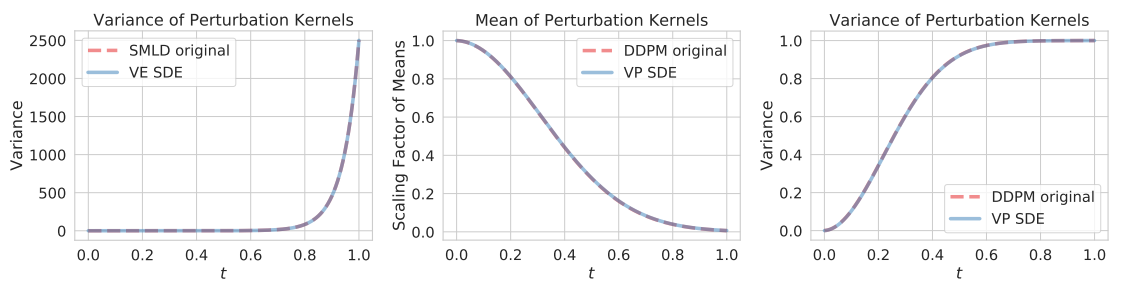
\includegraphics[width=0.9\linewidth]{figures/5.png}
    \caption{Các nhân gây xáo trộn rời rạc theo thời gian và phiên bản tổng quát dạng liên tục khớp với nhau một cách chính xác.
    Hình bên trái so sánh phương sai của nhân gây xáo trộn SMLD và VE SDE.
    Hình ở giữa so sánh hệ số nhân của trung bình của nhân gây xáo trộn của DDPM và VP SDE.
    Hình bên phải so sánh phương sai của nhân gây xáo trộn cho DDPM và VP SDE.}
    \label{fig:5}
\end{figure}

Với mô hình DDPM, $\lbrace \beta_i \rbrace_{i=1}^N$ thường là một dãy số học với $\beta_i = \dfrac{\bar{\beta}_{\min}}{N} + \dfrac{i-1}{N(N-1)}(\bar{\beta}_{\max}-\bar{\beta}_{\min})$ với $i=1, 2, \dots, N$.
Vì vậy, $\beta(t) = \bar{\beta}_{\min} + t (\bar{\beta}_{\max} - \bar{\beta}_{\min})$ với $t \in \lbrack 0, 1 \rbrack$ trong giới hạn $N \rightarrow \infty$.
Tương với với khởi tạo sau của VP SDE:

\begin{equation} \label{eq:32}
    d \bold{x} = -\dfrac{1}{2} \big( \bar{\beta}_{\min} + t (\bar{\beta}_{\max} - \bar{\beta}_{\min})) \bold{x} dt + \sqrt{\bar{\beta}_{\min} + t (\bar{\beta}_{\max} - \bar{\beta}_{\min})} d \bold{w}, t \in \lbrack 0, 1 \rbrack
\end{equation}

với $\bold{x}(0) \sim p_{\mathrm{data}}(\bold{x})$.
Trong thử nghiệm của ta, ta đặt $\bar{\beta}_{\min}=0.1$ và $\bar{\beta}_{\max}=20$ để khớp với cài đặt trong \citep{ho2020denoising}.
Nhân gây xáo trộn được cho bởi công thức:

\begin{equation} \label{eq:32}
    p_{0t} (\bold{x} \vert \bold{x}(0)) = \mathcal{N} \Big( \bold{x}(t); e^{-\dfrac{1}{4}t^2 (\bar{\beta}_{\max} - \bar{\beta}_{\min})-\dfrac{1}{2}t \bar{\beta}_{\min}} \bold{x}(0), \bold{I} - \bold{I} e^{-\dfrac{1}{2}t^2 (\bar{\beta}_{\max} - \bar{\beta}_{\min}) - t \bar{\beta}_{\min}} \Big)
\end{equation}

Đối với DDPM, không có vấn đề gián đoạn với VP SDE tuy nhiên có các vấn đề không ổn định số học cho quá trình huấn luyện và lấy mẫu tại $t=0$ vì hiện tượng triệt tiêu phương sai của $\bold{x}(t)$ khi $t \rightarrow 0$.
Vì vậy, cũng như VE SDE, ta chỉ tính toán ở khoảng $t \in \lbrack \epsilon, 1 \rbrack$ với một số $\epsilon > 0$ nhỏ.
Khi lấy mẫu, ta chọn $\epsilon = 10^{-3}$ nê phương sai của $\bold{x}(\epsilon)$ trong VP SDE khớp với phương sai của $\bold{x}_1$ trong DDPM.
Khi huấn luyện và tính độ hợp lý, ta chọn $\epsilon = 10^{-5}$ về mặt thực nghiệm cho kết quả tốt hơn.

Để kiểm tra tính đúng đắn của phương trình SDE tổng quát đối với SMLD và DDPM, ta so sánh nhân gây xáo trộn của SDÉ và xích Markov rời rạc ban đầu ở hình \ref{fig:5}.
Mô hình SMLD và DDPM đều sử dụng $N=1000$ ngưỡng nhiễu.
Đối với SMLD, ta chỉ cần so sánh phương sai của nhân gây xáo trộn khi cùng trung bình.
Đối với DDPM, ta so sánh hệ số nhân của trung bình và phương sai.
Như ở trong hình \ref{fig:5}, nhân gây xáo trộn rời rạc của mô hình SMLD và DDPM rất khớp với nhân gây xáo trộn thu được từ VE và VP SDE.

\begin{equation}
    p_{0t}(\bold{x}(t) \vert \bold{x}(0)) = \mathcal{N} \Big( \bold{x}(t); e^{-\dfrac{1}{4}t^2 (\bar{\beta}_{\max} - \bar{\beta}_{\min}) - \dfrac{1}{2}t\bar{\beta}_{\min}} \bold{x}(0), \lbrack 1 - e^{-\dfrac{1}{2}t^2 (\bar{\beta}_{\max} - \bar{\beta}_{\min} - t\bar{\beta}_{\min})} \rbrack^2 \bold{I} \Big)
\end{equation}

Ta cũng chỉ tính toán trên khoảng $\lbrack \epsilon, 1 \rbrack$ đối với VP SDE.

Về mặt thực nghiệm, ta quan sát một số $\epsilon$ nhỏ hơn về mặt tổng quát thu được độ hợp lý tốt hơn với tất cả các SDE.
Khi lấy mẫu, rất quan trọng khi sử dụng một số $\epsilon$ hợp lý để cho kết quả Inception và FID tốt hơn mặc dù đối với nhiều giá trị $\epsilon$ khác nhau các mẫu nhìn rất tương đương đối với mắt người. 


\section{Dòng xác suất phương trình ODE} \label{D}

\subsection{Diễn giải công thức} \label{D.1}

Ý tưởng của dòng xác suất phương trình ODE được lấy cảm hứng bởi \citep{maoutsa2020interacting} và ta có thể tìm thấy một vài trường hợp đơn giản hóa trong công trình này.
Tiếp theo ta sẽ cung cấp diễn giải công thức cho phương trình ODE tổng quát ở công thức \ref{eq:17}.
Ta xét phương trình SDE trong công thức \ref{eq:15} có dạng dưới đây:

\begin{equation*}
    d \bold{x} = \bold{f} (\bold{x}, t) dt + \bold{G}(\bold{x}, t) d \bold{w}
\end{equation*}

với $\bold{f}(., t): \mathbb{R}^d \rightarrow \mathbb{R}^d$ và $\bold{G}(., t): \mathbb{R}^d \rightarrow \mathbb{R}^{d\times d}$.
Hàm mật độ xác suất cận biên $p_t(\bold{x}(t))$ tiến triển theo phương trình Kolmogorov thuận (phương trình Fokker-Plank) \citep{oksendal2003stochastic}

\begin{equation} \label{eq:35}
    \dfrac{\partial p_t(\bold{x})}{\partial t} = - \sum_{i=1}^d \dfrac{\partial}{\partial x_i} \lbrack f_i (\bold{x}, t)p_t(\bold{x}) \rbrack + \dfrac{1}{2} \sum_{i=1}^d \sum_{j=1}^d \dfrac{\partial^2}{\partial x_i \partial x_j} \Big \lbrack \sum_{k=1}^d G_{ik} (\bold{x}, t) G_{jk}(\bold{x}, t) p_t (\bold{x}) \Big \rbrack
\end{equation}

Ta có thể viết lại công thức \ref{eq:35} để thu được:

\begin{equation} \label{eq:36}
    \begin{aligned}
        \dfrac{\partial p_t(\bold{x})}{\partial t} &= - \sum_{i=1}^d \dfrac{\partial}{\partial x_i} \lbrack f_i (\bold{x}, t)p_t(\bold{x}) \rbrack + \dfrac{1}{2} \sum_{i=1}^d \sum_{j=1}^d \dfrac{\partial^2}{\partial x_i \partial x_j} \Big \lbrack \sum_{k=1}^d G_{ik} (\bold{x}, t) G_{jk}(\bold{x}, t) p_t (\bold{x}) \Big \rbrack \\
        &= - \sum_{i=1}^d \dfrac{\partial}{\partial x_i} \lbrack f_i (\bold{x}, t)p_t(\bold{x}) \rbrack + \dfrac{1}{2} \sum_{i=1}^d \dfrac{\partial}{\partial x_i} \Big \lbrack \dfrac{\partial}{\partial x_j} \Big \lbrack \sum_{k=1}^d G_{ik} (\bold{x}, t) G_{jk}(\bold{x}, t) p_t (\bold{x}) \Big \rbrack \Big \rbrack
    \end{aligned}
\end{equation}

Ta cần chú ý rằng:

\begin{equation*}
    \begin{aligned}
        &\sum_{i=1}^d \dfrac{\partial}{\partial x_i} \Big \lbrack \dfrac{\partial}{\partial x_j} \Big \lbrack \sum_{k=1}^d G_{ik} (\bold{x}, t) G_{jk}(\bold{x}, t) p_t (\bold{x}) \Big \rbrack \\
        =& \sum_{i=1}^d \dfrac{\partial}{\partial x_i} \Big \lbrack \dfrac{\partial}{\partial x_j} \Big \lbrack \sum_{k=1}^d G_{ik} (\bold{x}, t) G_{jk}(\bold{x}, t) \Big \rbrack p_t (\bold{x}) + \sum_{j=1}^d \sum_{k=1}^d G_{ik}(\bold{x}, t) G_{jk}(\bold{x}, t) p_t(\bold{x}) \dfrac{\partial}{\partial x_j} \log p_t(\bold{x}) \\
        =& p_t(\bold{x}) \nabla . \lbrack \bold{G}(\bold{x}, t) \bold{G}(\bold{x}, t)^T \rbrack + p_t(\bold{x}) \bold{G}(\bold{x}, t) \bold{G}(\bold{x}, t)^T \nabla_{\bold{x}} \log p_t (\bold{x})
    \end{aligned}
\end{equation*}

dựa vào công thức trên ta tiếp tục viết lại công thức \ref{eq:36} thu được:

\begin{equation} \label{eq:37}
    \begin{aligned}
        \dfrac{\partial p_t (\bold{x})}{\partial t} &= - \sum_{i=1}^d \lbrack f_i (\bold{x}, t) p_t(\bold{x}) \rbrack + \dfrac{1}{2} \sum_{i=1}^d \sum_{j=1}^d \dfrac{\partial^2}{\partial x_i \partial x_j} \Big \lbrack \sum_{k=1}^d G_{ik} (\bold{x}, t) G_{jk}(\bold{x}, t) p_t (\bold{x}) \Big \rbrack \\
        &= - \sum_{i=1}^d \lbrack f_i (\bold{x}, t) p_t(\bold{x}) \rbrack + \dfrac{1}{2} \sum_{i=1}^d \dfrac{\partial}{\partial x_i} \Big \lbrack p_t(\bold{x}) \nabla . \lbrack \bold{G}(\bold{x}, t) \bold{G}(\bold{x}, t)^T \rbrack + p_t(\bold{x}) \bold{G}(\bold{x}, t) \bold{G}(\bold{x}, t)^T \nabla_{\bold{x}} \log p_t (\bold{x}) \Big \rbrack \\
        &= -\sum_{i=1}^d \dfrac{\partial}{\partial x_i} \Big \lbrack f_i(\bold{x}, t) p_t(\bold{x}) - \dfrac{1}{2} \Big \lbrack \nabla . \lbrack \bold{G}(\bold{x}, t) \bold{G}(\bold{x}, t)^T \rbrack + \bold{G}(\bold{x}, t) \bold{G}(\bold{x}, t)^T \nabla_{\bold{x}} \log p_t(\bold{x})  \Big \rbrack p_t(\bold{x}) \Big \rbrack \\
        &= - \sum_{i=1}^d \dfrac{\partial}{\partial x_i} \lbrack \tilde{f}_i (\bold{x}, t) p_t(\bold{x}) \rbrack
    \end{aligned}
\end{equation}

với ta định nghĩa:

\begin{equation*}
    \tilde{\bold{f}}(\bold{x}, t) := \bold{f}(\bold{x}, t) - \dfrac{1}{2} \nabla . \lbrack \bold{G}(\bold{x}, t) \bold{G}(\bold{x}, t)^T \rbrack - \dfrac{1}{2} \bold{G}(\bold{x}, t) \bold{G}(\bold{x}, t)^T \nabla_{\bold{x}} \log p_t(\bold{x})
\end{equation*}

Kiểm tra công thức \ref{eq:37}, ta quan sát thấy rằng công thức này tương đương với phương trình Kolmogorov thuận của phương trình SDE với $\tilde{\bold{G}} (\bold{x}, t) := \bold{0}$(Phương trình Kolmogorov thuận tỏng trường hợp này còn được gọi là phương trình Liouville)

\begin{equation*}
    d \bold{x} = \tilde{\bold{f}} (\bold{x}, t) dt + \tilde{\bold{G}}(\bold{x}, t) d \bold{w}
\end{equation*}

về cơ bản là một phương trình ODE:

\begin{equation*}
    d \bold{x} = \tilde{\bold{f}}(\bold{x}, t) dt
\end{equation*}

có cùng dòng xác suất ODE được cho bởi công thức \ref{eq:17}.
Vì vậy, ta đã chỉ ra rằng dòng xác suất ODE ở công thức \ref{eq:17} dẫn đến cùng hàm mật độ xác suất cận biên $p_t(\bold{x})$ với phương trình SDE ở công thức \ref{eq:15}.

\subsection{Tính toán độ hợp lý} \label{D.2}

Dòng xác suất của phương trình ODE trong công thức \ref{eq:17} có dạng sau khi ta thế điểm số $\nabla_{\bold{x}} \log p_t (\bold{x})$ với mô hình dựa trên điểm số phụ thuộc vào thời gian $\bold{s}_{\bold{\theta}}(\bold{x}, t)$:

\begin{equation} \label{eq:38}
    d \bold{x} = \underbrace{\Bigg \lbrace \bold{f}(\bold{x}, t) - \dfrac{1}{2} \nabla . \lbrace \bold{G}(\bold{x}, t) \bold{G}(\bold{x}, t)^T - \dfrac{1}{2} \bold{G}(\bold{x}, t) \bold{G}(\bold{x}, t)^T \bold{s}_{\bold{\theta}} (\bold{x}, t) \rbrace \Bigg \rbrace}_{=: \tilde{\bold{f}}(\bold{x}, t)} dt
\end{equation}

Với công thức thay đổi tức thời của các biến \citep{chen2018neural}, ta có thể tính log của độ hợp lý $p_0 (\bold{x})$ sử dụng:

\begin{equation} \label{eq:39}
    \log p_0 (\bold{x}(0)) = \log p_T (\bold{x}(T)) + \int_{0}^{T} \nabla . \tilde{\bold{f}}(\bold{x}(t), t) dt
\end{equation}

với biến ngẫu nhiên $\bold{x}(t)$ là một hàm của $t$ có thể thu được bằng cách giải dòng xác suất phương trình ODE ở công thức \ref{eq:38}.
Trong nhiều trường hợp việc tính $\nabla . \tilde{\bold{f}}_{\bold{\theta}}(\bold{x}, t)$ có chi phí tính toán khá đắt, ta theo phương pháp của \citep{grathwohl2018ffjord} để ước lượng đại lượng này với bộ ước lượng truy vết Skilling - Hutchinson \citep{skilling1989eigenvalues,hutchinson1989stochastic}.
Cụ thể, ta có:

\begin{equation} \label{eq:40}
    \nabla . \tilde{\bold{f}}_{\bold{\theta}}(\bold{x}, t) = \mathbb{E}_{p(\boldsymbol{\epsilon})} \lbrack \boldsymbol{\epsilon}^T \nabla \tilde{\bold{f}}_{\bold{\theta}} (\bold{x}, t) \boldsymbol{\epsilon} \rbrack
\end{equation}

với $\nabla \tilde{\bold{f}}_{\bold{\theta}}$ ký hiệu là ma trận Jacobi của $\tilde{\bold{f}}(., t)$ và biến ngẫu nhiên $\boldsymbol{\epsilon}$ thỏa mãn $\mathbb{E}_{p(\boldsymbol{\epsilon})} \lbrack \boldsymbol{\epsilon} \rbrack = \bold{0}$ và $\Cov_{p(\boldsymbol{\epsilon})} \lbrack \boldsymbol{\epsilon} \rbrack = \bold{I}$.
Tích của vector và ma trận Jacobi $\boldsymbol{\epsilon}^T \nabla \tilde{\bold{f}}_{\bold{\theta}}(\bold{x}, t)$ có thể được tính một cách hiệu quả sử dụng đạo hàm tự động chế độ ngược, xấp xỉ với chi phí tính $\tilde{\bold{f}}(\bold{x}, t)$.
Kết quả là ta có thể lấy mẫu $\boldsymbol{\epsilon} \sim p(\boldsymbol{\epsilon})$ và sau đó tính ước lượng không chệch hiệu quả của $\nabla . \tilde{\bold{f}}_{\bold{\theta}}(\bold{x}, t)$ sử dụng $\boldsymbol{\epsilon}^T \nabla \tilde{\bold{f}}_{\bold{\theta}} (\bold{x}, t) \boldsymbol{\epsilon}$.
Khi ước lượng này không chệch, ta có thể đạt đến một sai số nhỏ bất kỳ bằng cách lấy trung bình trên một số đủ lớn lần chạy.
Vì vậy, bằng cách áp dụng bộ ước lượng Skilling - Hutchinson ở công thức \ref{eq:40} cho công thức \ref{eq:39}, ta có thể tính log của độ hợp lý với độ chính xác bất kỳ.

Trong thử nghiệm của ta, ta sử dụng bộ giải RK45 ODE \citep{dormand1980family} được cung cấp bởi hàm scipy.integrate.solve\_ivp trong mọi trường hợp.
Giá trị bits/dim trong bảng \ref{tab:2} được tính với atol=1e-5 và rtol=1e-5 cũng như \citep{grathwohl2018ffjord}.
Để thu được kết quả độ hợp lý của mô hình trong bảng \ref{tab:2}, ta lấy trung bình bits/dim thu được trên tập test trên năm lần chạy khác nhau với $\epsilon=10^{-5}$ (định nghĩa $\epsilon$ ở phụ lục ).

\subsection{Lấy mẫu dòng xác suất} \label{D.3}

Giả sử ta có phương trình SDE thuận:

\begin{equation*}
    d \bold{x} = \bold{f}(\bold{x}, t) d t + \bold{G}(t) d \bold{w}
\end{equation*}

và phiên bản rời rạc hóa của phương trình này:

\begin{equation} \label{eq:41}
    \bold{x}_{i+1} = \bold{x}_i + \bold{f}_i(\bold{x}_i) + \bold{G}_i \bold{z}_i, i = 0, 1, \dots, N - 1
\end{equation}

với $\bold{z}_i \sim \mathcal{N}(\bold{0}, \bold{I})$.
Ta giả định lịch trình rời rạc hóa của thời gian được cố định từ trước,
và ta bỏ qua sự phụ thuộc vào $\Delta t$ vào ký hiệu của $\bold{f}_i$ và $\bold{G}_i$.
Sử dụng công thức \ref{eq:17}, ta thu được dòng xác suất phương trình ODE:

\begin{equation} \label{eq:42}
    d \bold{x} = \Bigg \lbrack \bold{f}(\bold{x}, t) - \dfrac{1}{2} \bold{G}(t) \bold{G}(t)^T \nabla_{\bold{x} \log p_t (\bold{x})} \Bigg \rbrack dt
\end{equation}

Ta có thể sử dụng một phương pháp số bất kỳ để tích hợp dòng xác suất phương trình ODE ngược theo thời gian cho việc sinh mẫu dữ liệu.
Cụ thể, ta đề xuất một phiên bản rời rạc hóa có dạng chức năng tương tự với phương trình \ref{eq:41}:

\begin{equation*}
    \bold{x}_i = \bold{x}_{i+1} - \bold{f}_{i+1}(\bold{x}_{i+1}) + \dfrac{1}{2} \bold{G}_{i+1} \bold{G}_{i+1}^T \bold{s}_{\bold{\theta}^{\ast}} (\bold{x}_{i+1}, i+1), i = 0, 1, \dots, N - 1
\end{equation*}

với mô hình dựa trên điểm số $\bold{s}_{\bold{\theta}^{\ast}}(\bold{x}_i, i)$ có điều kiện dựa trên bước lặp thứ $i$.
Đây là một quy tắc lặp tất định.
Không như các bộ lấy mẫu khuếch tán ngược hoặc ancestral sampling, không có bất kỳ tính ngẫu nhiên nào một khi mẫu ban đầu $\bold{x}_N$ thu được từ phân phối tiên nghiệm.
Khi áp dụng vào mô hình SMLD, ta có thể thu được luật lặp sau cho lấy mẫu dòng xác suất:

\begin{equation} \label{eq:43}
    \bold{x}_i = \bold{x}_{i+1} + \dfrac{1}{2} (\sigma_{i+1}^2 - \sigma_i^2) \bold{s}_{\bold{\theta}^{\ast}} (\bold{x}_{i+1}, \sigma_{i+1}), i = 0, 1, \dots, N - 1
\end{equation}

Tương tự, với mô hình DDPM, ta có:

\begin{equation} \label{eq:44}
    \bold{x}_i = (2 - \sqrt{1 - \beta_{i+1}}) \bold{x}_{i+1} + \dfrac{1}{2} \beta_{i+1} \bold{s}_{\bold{\theta}^{\ast}} (\bold{x}_{i+1}, i + 1), i = 0, 1, \dots, N - 1
\end{equation}

\subsection{Lấy mẫu với bộ giải hộp đen phương trình ODE} \label{D.4}

Để tạo ra hình \ref{fig:3}, ta sử dụng một mô hình DDPM được huấn luyện trên tập CelebA-HQ 256$\times$256 với cùng cấu hình trong \citep{ho2020denoising}.
Tất cả các điểm FID của mô hình của ta trong bảng \ref{tab:2} được tính trên các mẫu từ bộ giải RK45 PDE được thực thi trong scipy.integrate.solve\_ivp với atol=1e-5 và rtol=1e-5.
Ta sử dụng $\epsilon=10^{-5}$ cho VE SDEs và $\epsilon=10^{-3}$ cho VP SDEs (phụ lục ).

Ngoài các kết quả nôi suy trong hình \ref{fig:3}, ta trình bày thêm các mẫu về can thiệp trong không gian ẩn ở hình \ref{fig:6} bao gồm nội suy và chia tỷ lệ nhiệt độ.
Mô hình được thử nghiệm là mô hình DDPM được huấn luyện với cùng cấu hình trong \citep{ho2020denoising}.

Mặc dù các bộ giải cho dòng xác suất phương trình ODE cho phép lấy mẫu nhanh, nhưng các mẫu thường có FID cao hơn (không tốt) hơn so với các bộ giải của phương trình SDE nếu không có bộ hiệu chỉnh được sử dụng.
Ta có các quan sát thực nghiệm cho cả hai chiến lược rời rạc hóa ở phụ lục \ref{D.3} và bộ giải ODE hộp đen được giới thiệu ở trên.
Hơn nữa, hiệu năng của bộ giải dòng xác suất phương trình ODE phụ thuộc vào lựa chọn của phương trình SDE - chất lượng mẫu của VE SDE kém hơn nhiều so với VP SDE đặc biệt là trên dữ liệu nhiều chiều 


\subsection{Mã hóa có thể nhận dạng duy nhất} \label{D.5}

Để kiểm tra tính đúng đắn, ta huấn luyện hai mô hình (ký hiệu là "mô hình A" và "mô hình B") với các kiến trúc khác nhau sử dụng VE SDE trên tập CIFAR-10.
Mô hình A là một mô hình NCSN++ với 4 lớp neuron trên từng độ phân giải được huấn luyện sử dụng hàm mục tiêu liên tục ở trong công thức \ref{eq:7} và mô hình B cũng giống hệt ngoại trừ sử dụng 8 lớp neuron trên từng độ phân giải.
Các cấu hình về mô hình ở phụ lục .

Ta báo cáo mã hóa ẩn thu được từ mô hình A và mô hình B cho các ảnh ngẫu nhiên trên tập CIFAR-10 trong hình \ref{fig:7}.
Trong hình \ref{fig:8}, ta chỉ ra rằng sự khác biệt giữa từng chiều và hệ số tương quan giữa các mã hóa ẩn trên 16 ảnh của tập CIFAR-10.
Các kết quả cho thấy với cùng đầu vào, mô hình A và mô hình B cung cấp các mã hóa rất giống nhau ở trên các chiều, mặc dù khác kiến trúc mô hình và cấu hình huấn luyện.

\section{Lấy mẫu khuếch tán ngược} \label{E}

Cho phương trình SDE thuận:

\begin{equation*}
    d \bold{x} = \bold{f}(\bold{x}, t) dt + \bold{G}(t) d \bold{w}
\end{equation*}

và giả định luật lặp sau là phiên bản rời rạc của phương trình vi phân trên:

\begin{equation} \label{eq:45}
    \bold{x}_{i+1} = \bold{x}_i + \bold{f}_i (\bold{x}_i) + \bold{G}_i \bold{z}_i, i = 0, 1, \dots, N - 1
\end{equation}

với $\bold{z}_i \sim \mathcal{N}(\bold{0}, \bold{I})$.
Ta giả định lịch trình rời rạc hóa của thời gian được cố định từ trước và ta có thể bỏ qua trong ký hiệu của $\bold{f}_i$ và $\bold{G}_i$.

Dựa trên công thức \ref{eq:45}, ta đề xuất rời rạc hóa phương trình SDE đảo ngược thời gian:

\begin{equation*}
    d \bold{x} = \lbrack \bold{f}(\bold{x}, t) - \bold{G}(t) \bold{G}(t)^T \nabla_{\bold{x}} \log p_t (\bold{x}) \rbrack dt + \bold{G}(t) d \bar{\bold{w}}
\end{equation*}

Với dạng tương tự, luật lặp cho $i \in \lbrace 0, 1, \dots, N -1 \rbrace$:

\begin{equation} \label{eq:46}
    \bold{x}_i = \bold{x}_{i+1} - \bold{f}_{i+1} (\bold{x}_{i+1}) + \bold{G}_{i+1} \bold{G}_{i+1}^T \bold{s}_{\boldsymbol{\theta}^{\ast}} (\bold{x}_{i+1}, i + 1) + \bold{G}_{i+1} \bold{z}_{i+1}
\end{equation}

với mô hình dựa trên điểm số đã được huấn luyện $\bold{x}_{\boldsymbol{\theta}^{\ast}}(\bold{x}_i, i)$ được lấy điều kiện trên bước lặp thứ $i$.

Khi áp dụng công thức \ref{eq:46} vào công thức \ref{eq:10} và công thức \ref{eq:20}, ta thu được một tập mới các bộ giải số cho phương trình VE và VP SDEs đảo ngược thời gian, kết quả tạo ra thuật toán lấy mẫu của phần "bộ dự đoán" ở trong thuật toán và thuật toán .
Ta đặt tên các phương pháp lấy mẫu này là (dựa trên chiến lược rời rạc hóa ở công thức \ref{eq:46}) bộ lấy mẫu khuếch tán ngược.

Như kỳ vọng, ancestral sampling của mô hình DDPM \citep{ho2020denoising} ở công thức \ref{eq:4} khớp với bộ khuếch tán ngược khi $\beta_i \rightarrow 0$ với mọi $i$ (điều này xảy ra khi $\Delta t \rightarrow 0$ khi $\beta_i = \bar{\beta}_i$ được trình bày ở phụ lục ), bởi vì:

\begin{equation*}
    \begin{aligned}
        \bold{x}_i &= \dfrac{1}{\sqrt{1 - \beta_{i+1}}}(\bold{x}_{i+1} + \beta_{i+1} \bold{s}_{\boldsymbol{\theta}^{\ast}}(\bold{x}_{i+1}, i+1)) + \sqrt{\beta_{i+1}} \bold{z}_{i+1} \\
        &= \Big( 1 + \dfrac{1}{2} \beta_{i+1} + o(\beta_{i+1}) \Big)(\bold{x}_{i+1} + \beta_{i+1} \bold{s}_{\boldsymbol{\theta}^{\ast}}(\bold{x}_{i+1}, i+1)) + \sqrt{\beta_{i+1}} \bold{z}_{i+1} \\
        &\approx \Big( 1 + \dfrac{1}{2}\beta_{i+1} \Big)(\bold{x}_{i+1} + \beta_{i+1} \bold{s}_{\boldsymbol{\theta}^{\ast}}(\bold{x}_{i+1}, i+1)) + \sqrt{\beta_{i+1}} \bold{z}_{i+1} \\
        &= \Big( 1 + \dfrac{1}{2}\beta_{i+1} \Big) \bold{x}_{i+1} + \beta_{i+1} \bold{s}_{\boldsymbol{\theta}^{\ast}} (\bold{x}_{i+1}, i + 1) + \dfrac{1}{2} \beta_{i+1}^2 \bold{s}_{\boldsymbol{\theta}^{\ast}} (\bold{x}_{i+1}, i+1) + \sqrt{\beta_{i+1}} \bold{z}_{i+1} \\
        &\approx \Big( 1 + \dfrac{1}{2}\beta_{i+1} \Big) \bold{x}_{i+1} + \beta_{i+1} \bold{s}_{\boldsymbol{\theta}^{\ast}} (\bold{x}_{i+1}, i + 1) + \sqrt{\beta_{i+1}} \bold{z}_{i+1} \\
        &= \Big \lbrack 2 - \Big ( 1 - \dfrac{1}{2} \beta_{i+1} \Big) \Big \rbrack \bold{x}_{i+1} + \beta_{i+1} \bold{s}_{\boldsymbol{\theta}^{\ast}}(\bold{x}_{i+1}, i+1) + \sqrt{\beta_{i+1}} \bold{z}_{i+1} \\
        &\approx \Big \lbrack 2 - \Big ( 1 - \dfrac{1}{2} \beta_{i+1} \Big) + o(\beta_{i+1}) \Big \rbrack \bold{x}_{i+1} + \beta_{i+1} \bold{s}_{\boldsymbol{\theta}^{\ast}}(\bold{x}_{i+1}, i+1) + \sqrt{\beta_{i+1}} \bold{z}_{i+1} \\
        &= (2 - \sqrt{1 - \beta_{i+1}}) \bold{x}_{i+1} + \beta_{i+1} \bold{s}_{\boldsymbol{\theta}^{\ast}}(\bold{x}_{i+1}, i+1) + \sqrt{\beta_{i+1}} \bold{z}_{i+1} \\
    \end{aligned}
\end{equation*}

Vì vậy, bộ lấy mẫu ancestral sampling ban đầu của công thức \ref{eq:4} về cơ bản là một phiên bản rời rạc hóa khác của cùng một phương trình SDE đảo ngược thời gian.
Điều này nhất quán với phương pháp lấy mẫu trong \citep{ho2020denoising} là một bộ giải số cho phương trình VP SDE đảo ngược thời gian trong khung làm việc liên tục của ta.

\begin{figure}[h!]
    \centering
    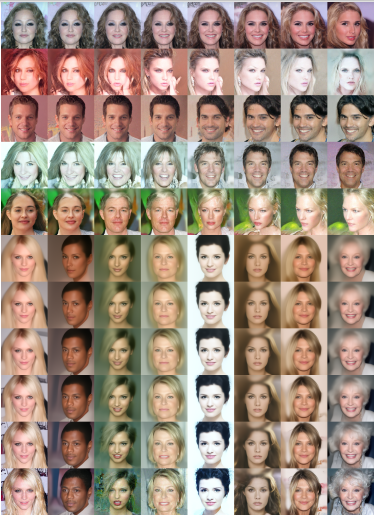
\includegraphics[height=0.7\textheight]{figures/6.png}
    \caption{Các mẫu từ dòng xác suất phương trình ODE cho VP SDE trên tập CelebA-HQ 256$\times$256.
    Các hàng trên: Nội suy cầu giữa các mẫu ngẫu nhiên.
    Các hàng dưới: thay đổi tham số nhiệt độ (giảm chuẩn trong embedding)}
    \label{fig:6}
\end{figure}

\begin{figure}[h!]
    \centering
    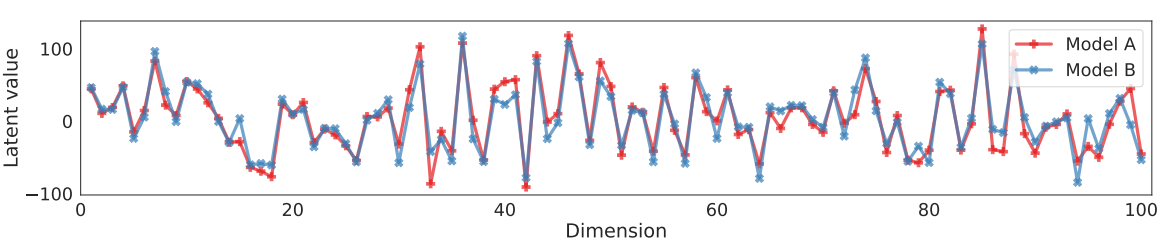
\includegraphics[width=0.8\linewidth]{figures/7.png}
    \caption{So sánh 100 chiều đầu tiên của mã hóa ẩn thu được từ một ảnh ngẫu nhiên trên tập CIFAR-10.
    "Mô hình A" và "mô hình B" được huấn luyện trên các kiến trúc khác nhau}
    \label{fig:7}
\end{figure}

\begin{figure}[h!]
    \centering
    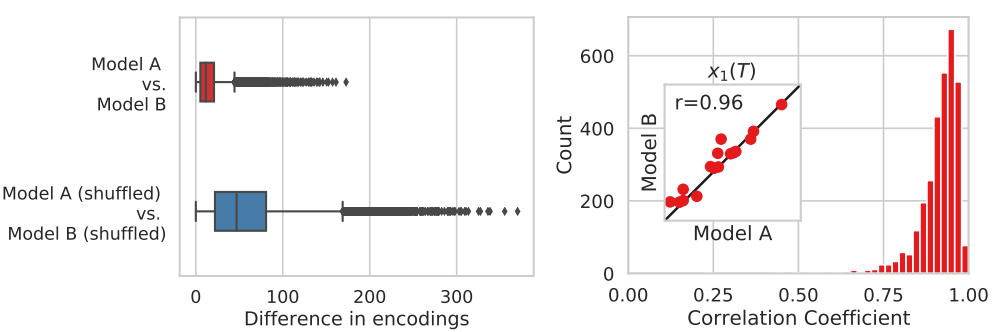
\includegraphics[width=0.8\linewidth]{figures/8.png}
    \caption{\textit{Trái:} Sự khác biệt về từng chiều giữa mã hóa thu được từ mô hình A và mô hình B.
    Ta cũng so sánh sự khác nhau giữa biểu diễn bị xáo trộn của hai mô hình.
    \textit{Phải:} Hệ số tương quan từng chiều của mã hóa thu được từ mô hình A và mô hình B.}
    \label{fig:8}
\end{figure}

\section{Ancestral Sampling cho mô hình SMLD} \label{F}

Phương pháp ancestral sampling cho mô hình DDPM có thể được áp dụng cho mô hình SMLD.
Ta sét một dãy các ngưỡng nhiễu $\sigma_1 < \sigma_2 < \dots < \sigma_N$ trong SMLD.
Bằng cách gây xáo trộn điểm dữ liệu $\bold{x}_0$ với các ngưỡng nhiễu này một cách tuần tự, ta thu được một xích Markov $\bold{x}_0 \rightarrow \bold{x}_1 \rightarrow \dots \rightarrow \bold{x}_N$ với:

\begin{equation*}
    p(\bold{x}_i \vert \bold{x}_{i-1}) = \mathcal{N}(\bold{x}_i; \bold{x}_{i-1}, (\sigma_i^2 - \sigma_{i-1}^2) \bold{I}), i = 1, 2, \dots, N
\end{equation*}

Ta giả sử $\sigma_0 = 0$ để đơn giản hóa ký hiệu.
Theo \citep{ho2020denoising}, ta có thể tính:

\begin{equation*}
    q(\bold{x}_{i-1} \vert \bold{x}_i, \bold{x}_0) = \mathcal{N} \Bigg( \bold{x}_{i-1}; \dfrac{\sigma_{i-1}^2}{\sigma_i^2} \bold{x}_i + \Big( 1 - \dfrac{\sigma_{i-1}^2}{\sigma_i^2} \Big) \bold{x}_0, \dfrac{\sigma_{i-1}^2 (\sigma_i^2 - \sigma_{i-1}^2)}{\sigma_i^2} \bold{I} \Bigg)
\end{equation*}

Nếu ta tham số hóa nhân chuyển tiếp ngược là $p_{\boldsymbol{\theta}}(\bold{x}_{i-1} \vert \bold{x}_i)=\mathcal{N}(\bold{x}_{i-1}; \boldsymbol{\mu}_{\boldsymbol{\theta}}(\bold{x}_i, i), \tau_i^2 \bold{I})$:

\begin{equation*}
    \begin{aligned}
        L_{t-1} &= \mathbb{E}_q \lbrack D_{\mathrm{KL}}(q(\bold{x}_{i-1}) \Vert p_{\boldsymbol{\theta}}(\bold{x}_{i-1} \vert \bold{x}_i)) \rbrack \\
        &= \mathbb{E}_q \Bigg \lbrack \dfrac{1}{2 \tau_i^2} \Bigg \lVert \dfrac{\sigma_{i-1}^2}{\sigma_i^2} \bold{x}_i + \big(1 - \dfrac{\sigma_{i-1}^2}{\sigma_i^2} \bold{x}_0 - \boldsymbol{\mu}_{\boldsymbol{\theta}} (\bold{x}_i, i) \big) \Bigg \rVert_2^2 \Bigg \rbrack + C \\
        &= \mathbb{E}_{\bold{x}_0, \bold{z}} \Bigg \lbrack \dfrac{1}{2 \tau_i^2} \Bigg \lVert \bold{x}_i(\bold{x}_0, \bold{z}) - \dfrac{\sigma_i^2 - \sigma_{i-1}^2}{\sigma_i} \bold{z} - \boldsymbol{\mu}_{\boldsymbol{\theta}} (\bold{x}_i (\bold{x}_0, \bold{z}), i) \Bigg \rVert_2^2 \Bigg \rbrack + C
    \end{aligned}
\end{equation*}

với $L_{t-1}$ là một thành phần biểu diễn của hàm mục tiêu ELBO (công thức 8 trong \citep{ho2020denoising}), C là một hằng số không phụ thuộc vào $\boldsymbol{\theta}, \bold{z} \sim \mathcal{N}(\bold{0}, \bold{I})$ và $bold{x}_i (\bold{x}_0, \bold{z})=\bold{x}_0 + \sigma_i \bold{z}$.
Vì vậy ta có thể tham số hóa $\boldsymbol{\mu}_{\boldsymbol{\theta}}(\bold{x}_i, i)$ qua công thức:

\begin{equation} \label{eq:47}
    \bold{x}_{i-1} = \bold{x}_i + (\sigma_i^2 - \sigma_{i-1}^2) \bold{s}_{\boldsymbol{\theta}^{\ast}} (\bold{x}_i, i) + \sqrt{\dfrac{\sigma_{i-1}^2 (\sigma_i^2 - \sigma_{i-1}^2)}{\sigma_i^2}} \bold{z}_i, i = 1, 2, \dots, N
\end{equation}

với $\bold{x}_N \sim \mathcal{N}(\bold{0}, \sigma_N^2 \bold{I}), \bold{\theta}^{\ast}$ ký hiệu tham số tối ưu của $\bold{s}_{\boldsymbol{\theta}}$ và $\bold{z}_i \sim \mathcal{N}(\bold{0}, \bold{I})$.
Ta gọi công thức \ref{eq:47} là phương pháp ancestral sampling cho mô hình SMLD.

\section{Bộ lấy mẫu dự đoán - hiệu chỉnh} \label{G}

\textbf{Lấy mẫu dự đoán - hiệu chỉnh (PC)} Bộ dự đoán có thể là bất kỳ bộ giải số nào cho phương trình SDE đảo ngược thời gian với chiến lược rời rạc hóa cố định.
Bộ hiệu chỉnh có thể là bất kỳ phương pháp MCMC nào dựa trên điểm số.
Trong quá trình lấy mẫu sử dụng PC, ta luân phiên chạy giữa bộ dự đoán và bộ hiệu chỉnh được miêu tả trong thuật toán \ref{alg:1}.
Ví dụ, khi sử dụng bộ giải phương trình SDE khuếch tán đảo ngược thời gian (phụ lục ) là bộ dự đoán, và tôi luyện động học Langevin \citep{song2019generative} là bộ hiệu chỉnh, ta có thuật toán \ref{alg:2} và thuật toán \ref{alg:3} cho VE và VP SDE tương ứng,
với $\lbrace \epsilon_i \rbrace_{i=0}^{N-1}$ là độ dài bước cho động học Langevin được trình bày bên Dưới

\begin{algorithm}[h!]
    \DontPrintSemicolon
    \KwIn{$N$: số bước rời rạc hóa cho phương trình SDE đảo ngược thời gian, $M$: số bước hiệu chỉnh}
    Khởi tạo $\bold{x}_N \sim p_T(\bold{x})$\;
    \For {$i \gets N - 1$ \KwSty{to} 0} {
        $\bold{x}_i \gets$ Predictor($\bold{x}_{i+1}$)\;
        \For {$j \gets 1$ \KwSty{to} M} {
            $\bold{x}_i \gets$ Corrector($\bold{x}_i$)\;
        }
    }
    \Return{$\bold{x}_0$}\;
    \caption{Bộ lấy mẫu dự đoán - hiệu chỉnh (PC)}
    \label{alg:1}
\end{algorithm}

\begin{algorithm}[h!]
    \DontPrintSemicolon
    $\bold{x}_N \sim \mathcal{N}(\bold{0}, \sigma_{\max}^2 \bold{I})$\;
    \For {$i \gets N - 1$ \KwSty{to} 0} {
        $\bold{x}_i^{\prime} \gets \bold{x}_{i+1} + (\sigma_{i+1}^2 - \sigma_i^2)\bold{s}_{\boldsymbol{\theta}}^{\ast}(\bold{x}_{i+1}, \sigma_{i+1})$\;
        $\bold{z} \sim \mathcal{N}(\bold{0}, \bold{I})$\;
        $\bold{x}_i \gets \bold{x}_i^{\prime} + \sqrt{\sigma_{i+1}^2 - \sigma_i^2} \bold{z}$\;
        \For{$j \gets 1$ \KwSty{to} $M$} {
            $\bold{z} \gets \mathcal{N}(\bold{0}, \bold{I})$\;
            $\bold{x}_i \gets \bold{x}_i + \epsilon_i \bold{s}_{\boldsymbol{\theta}^{\ast}}(\bold{x}_i, \sigma_i) + \sqrt{2 \epsilon_i} \bold{z}$\;
        }
    }
    \Return{$\bold{x}_0$}\;
    \caption{Lấy mẫu PC (VE SDE)}
    \label{alg:2}
\end{algorithm}

\begin{algorithm}[h!]
    \DontPrintSemicolon
    $\bold{x}_N \sim \mathcal{N}(\bold{0}, \bold{I})$\;
    \For {$i \gets N - 1$ \KwSty{to} 0} {
        $\bold{x}_i^{\prime} \gets (2 - \sqrt{1 - \beta_{i+1}}) \bold{x}_{i+1} + \beta_{i+1} \bold{s}_{\boldsymbol{\theta}^{\ast}}(\bold{x}_{i+1}, i+1)$\;
        $\bold{z} \sim \mathcal{N}(\bold{0}, \bold{I})$\;
        $\bold{x}_i \gets \bold{x}_i^{\prime} + \sqrt{\beta_{i+1}} \bold{z}$\;
        \For{$j \gets 1$ \KwSty{to} $M$} {
            $\bold{z} \gets \mathcal{N}(\bold{0}, \bold{I})$\;
            $\bold{x}_i \gets \bold{x}_i + \epsilon_i \bold{s}_{\boldsymbol{\theta}^{\ast}}(\bold{x}_i, \sigma_i) + \sqrt{2 \epsilon_i} \bold{z}$\;
        }
    }
    \Return{$\bold{x}_0$}\;
    \caption{Lấy mẫu PC (VP SDE)}
    \label{alg:3}
\end{algorithm}

\textbf{Thuật toán hiệu chỉnh} Ta đặt lịch trình cho tôi luyện động học Langevin trong \citep{song2019generative}, nhưng sắp xếp lại với một vài chỉnh sửa để tăng khả năng giải thích và hiệu năng thực nghiệm.
Ta cung cấp các thuật toán hiệu chỉnh trong thuật toán \ref{alg:4} và thuật toán \ref{alg:5} tương ứng, ta gọi $r$ là tỷ số "signal to noise".
Ta xác định các độ dài bước $\epsilon$ sử dụng chuẩn của nhiễu Gauss $\lVert z \rVert_2$, chuẩn của mô hình dựa trên điểm số $\lVert \bold{s}_{\boldsymbol{\theta}^{\ast}} \rVert_2$ và tỷ lệ signal-to-noise $r$.
Khi lấy mẫu một nhóm lớn các mẫu cùng một lúc, ta thay chuẩn $\lVert . \rVert_2$ với trung bình của chuẩn trong nhóm.
Khi kích thước nhóm nhỏ, ta thay $\lVert \bold{z} \rVert_2$ với $\sqrt{d}$, với $d$ là số chiều của $\bold{z}$.



\begin{algorithm}[h!]
    \DontPrintSemicolon
    \KwIn{$\lbrace \sigma_i \rbrace_{i=1}^N, r, N, M$}
    $\bold{x}_N^0 \sim \mathcal{N}(\bold{0}, \sigma_{\max}^2 \bold{I})$\;
    \For{$i \gets N$ \KwSty{to} 1} {
        \For{$j \gets 1$ \KwSty{to} $M$} {
            $\bold{z} \gets  \mathcal{N}(\bold{0}, \bold{I})$\;
            $\bold{g} \gets \bold{s}_{\boldsymbol{\theta}^{\ast}}(\bold{x}_i^{j-1}, \sigma_i)$\;
            $\epsilon \gets 2 (r \lVert \bold{z} \rVert_2 / \lVert g \rVert_2)^2$\;
            $\bold{x}_i^j \gets \bold{x}_i^{j-1} + \epsilon \bold{g} + \sqrt{2 \epsilon} \bold{z}$\;
        }
        $\bold{x}_{i-1}^0 \gets \bold{x}_i^M$\;
    }
    \Return{$\bold{x}_0^0$}\;
    \caption{Thuật toán hiệu chỉnh (VE SDE)}
    \label{alg:4}
\end{algorithm}

\begin{algorithm}[h!]
    \DontPrintSemicolon
    \KwIn{$\lbrace \sigma_i \rbrace_{i=1}^N, r, N, M$}
    $\bold{x}_N^0 \sim \mathcal{N}(\bold{0}, \bold{I})$\;
    \For{$i \gets N$ \KwSty{to} 1} {
        \For{$j \gets 1$ \KwSty{to} $M$} {
            $\bold{z} \gets  \mathcal{N}(\bold{0}, \bold{I})$\;
            $\bold{g} \gets \bold{s}_{\boldsymbol{\theta}^{\ast}}(\bold{x}_i^{j-1}, i)$\;
            $\epsilon \gets 2 \alpha_i (r \lVert \bold{z} \rVert_2 / \lVert g \rVert_2)^2$\;
            $\bold{x}_i^j \gets \bold{x}_i^{j-1} + \epsilon \bold{g} + \sqrt{2 \epsilon} \bold{z}$\;
        }
        $\bold{x}_{i-1}^0 \gets \bold{x}_i^M$\;
    }
    \Return{$\bold{x}_0^0$}\;
    \caption{Thuật toán hiệu chỉnh (VP SDE)}
    \label{alg:5}
\end{algorithm}

\textbf{Khử nhiễu} Cho cả hai mô hình SMLD và DDPM, các mẫu dữ liệu được sinh ra thường bao gồm một lượng nhỏ nhiễu rất khó được phát hiện bởi con người.
Được chú ý bởi \cite{jolicoeur2020adversarial}, FID có thể tệ hơn đáng kể nếu không được loại bỏ nhiễu này.
Sự nhạy cảm với nhiễu cũng là một lý do vì sao mô hình NCNS được huấn luyện với SMLD hoạt động kém hơn so với mô hình DDPM về chỉ số FID, bởi vì các mô hình trước không sử dụng bước khử nhiễu khi kết thúc lấy mẫu trong khi các mô hình mới có khử nhiễu.
Trong tất cả các thử nghiệm của công trình này, ta đảm bảo có bước khử nhiễu khi kết thúc quá trình lấy mẫu, sử dụng công thức Tweedie \cite{efron2011tweedie}

\begin{figure}[h!]
    \centering
    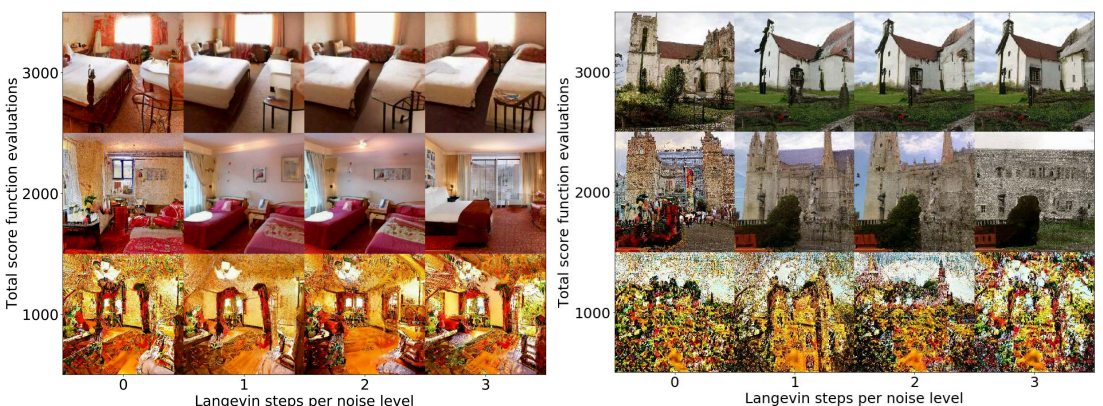
\includegraphics[width=0.8\linewidth]{figures/9.png}
    \caption{Lấy mẫu PC cho tập LSUN bedroom và LSUN church.
    Trục thẳng đứng tương ứng với tổng chi phí tính toán, trục nằm ngang biểu diễn lượng tính toán dành cho bộ hiệu chỉnh.
    Các mẫu là tốt nhất khi chi phí tính toán chi đều giữa bộ dự đoán và bộ hiệu chỉnh}
    \label{fig:9}
\end{figure}

\textbf{Huấn luyện} Ta sử dụng cùng kiến trúc trong \citep{ho2020denoising} cho mô hình dựa trên điểm số của ta.
Cho VE SDE, ta huấn luyện một moohinhf với hàm mục tiêu SMLD gốc trong công thức \ref{eq:1}, tương tự cho VP SDE,
ta sử dụng hàm mục tiêu DDPM ban đầu trong công thức \ref{eq:3}.
Ta áp dụng số ngưỡng nhiễu là 1000 ngưỡng nhiễu cho huấn luyện các mô hình.
Kết quả ở trong hình \ref{fig:9}, ta huấn luyện mô hình NCSN++ (được trình bày ở phụ lục ) trên tạp LSUN 256 $\times$ 256 bedroom và LSUN 256 $\times$ 256 church \citep{yu2015lsun} với VESDE và hàm mục tiêu liên tục ở công thức \ref{eq:7}.
Batch size được cố định là 128 trên tập CIFAR-10 và 64 trên tập LSUN.

\textbf{Các phương pháp nội suy ad-hoc cho các ngưỡng nhiễu} Mô hình trong thử nghiệm ngày được huấn luyện với 1000 ngưỡng nhiễu.
Để thu được kết quả cho P2000 (bộ lấy mẫu chỉ dự đoán sử dụng 2000 bước) yêu cầu 2000 ngưỡng nhiễu,
ta cần nội suy giữa 1000 ngưỡng nhiễu tại thời điểm chạy suy luận.
Kiến trúc cụ thể cho mô hình dựa trên điểm số điều kiện vào nhiễu trong \citep{ho2020denoising} sử dụng sinusoidal positional embeddings cho mô hình hóa điều kiện trên số bước là số nguyên.
Điều này cho phép ta nội suy giữa các ngưỡng nhiễu trong lúc chạy suy luận theo cách ad-hoc (trong khi rất khó để làm như vậy cho các kiến trúc khác như kiến trúc trong \citep{song2019generative}).
Cụ thheer, cho mô hình SMLD, ta giữ $\sigma_{\min}$ và $\sigma_{\max}$ cố định và tăng gấp đôi số bước thời gian.
Đối với mô hình DDPM, ta giảm một nửa $\beta_{\min}$ và $\beta_{\max}$ trong khi tăng ấp đôi số bước thời gian.
Giả sử $\lbrace \bold{s}_{\boldsymbol{\theta}}(\bold{x}, i) \rbrace_{i=0}^{N-1}$ là một mô hình dựa trên điểm số được huấn luyện trên $N$ bước thời gian và đặt $\lbrace \bold{s}_{\boldsymbol{\theta}}(\bold{x}, i)^{\prime} \rbrace_{i=0}^{2N-1}$ ký hiệu là mô hình dựa trên điểm số được nội suy tương ứng tại $2N$ bước thời gian.
Ta kiểm tra hai chiến lược nội suy cho các bước thời gian, nội suy tuyến tính với $\bold{s}_{\boldsymbol{\theta}}^{\ast} (\bold{x}, i)= \bold{s}_{\boldsymbol{\theta}}(\bold{x}, i/2)$ và nội suy làm tròn với $\bold{s}_{\boldsymbol{\theta}}^{\ast} (\bold{x}, i)= \bold{s}_{\boldsymbol{\theta}}(\bold{x}, \floor*{i/2})$.
Ta cung cấp các kết quả với nội suy tuyến tính trong bảng \ref{tab:1} và kết quả cho nội suy làm tròn ở bảng \ref{tab:4}.
Ta quan sát các phương pháp nội suy khác nhau cho kết quả khác nhau nhưng vẫn duy trì xung hướng chung phương pháp dự đoán - hiệu chỉnh cho kết quả tốt hơn chỉ sử dụng bộ dự đoán hoặc bộ hiệu chỉnh.



\begin{table}[h!]
    \centering
    \caption{So sánh các bộ lấy mẫu khác nhau trên tập CIFAR-10, với "P2000" sử dụng nội suy làm tròn giữa các ngưỡng nhiễu.
    Trung bình và phương sai được tính dựa trên năm lần chạy lấy mẫu}
    \resizebox{\columnwidth}{!}{
        \begin{tabular}{c|c|c|c|c|c|c|c|c}
            \hline
            & \multicolumn{4}{|c|}{Variance Exploding SDE (SMLD)} & \multicolumn{4}{|c}{Variance Preserving SDE (DDPM)} \\
            \hline
            FID $\downarrow$ & P1000 & P2000 & C2000 & PC1000 & P1000 & P2000 & C2000 & PC1000 \\
            \hline
            ancestral sampling & 4.98 $\pm$ .06 & 4.92 $\pm$ .02 & \multirow{3}{*}{20.43 $\pm$ .07} & \textbf{3.62} $\pm$ \textbf{.03} & 3.24 $\pm$  .02 & \textbf{3.11} $\pm$ \textbf{.03} & \multirow{3}{*}{19.06 $\pm$ .06} & 3.21 $\pm$ .02 \\
            reverse diffusion & 4.79 $\pm$ .07 & 4.72 $\pm$ .07 & & \textbf{3.60} $\pm$ \textbf{.02} & 3.21 $\pm$  .02 & \textbf{3.10} $\pm$ \textbf{.03} & & 3.18 $\pm$ .01 \\
            probability flow & 15.41 $\pm$ .15 & 12.87 $\pm$ .09 & & \textbf{3.51} $\pm$ \textbf{.04} & 3.59 $\pm$  .04 & 3.25 $\pm$ .04 & & \textbf{3.06} $\pm$ \textbf{.03} \\
            \hline
        \end{tabular}
    }
    \label{tab:4}
\end{table}

\begin{table}[h!]
    \centering
    \caption{Tỷ lệ signal-to-noise tối cho cho các bộ lấy mẫu khác nhau.
    "P1000" và "P2000": lấy mẫu chỉ sử dụng bộ dự đoán sử dụng 1000 hoặc 2000 bước thời gian.
    "C2000": lấy mẫu chỉ sử dụng bộ hiệu chỉnh sử dụng 2000 bước.
    "PC1000": lấy mẫu sử dụng dự đoán - hiệu chỉnh với 1000 bước dự đoán và 1000 bước hiệu chỉnh}
    \resizebox{\columnwidth}{!}{
        \begin{tabular}{c|c|c|c|c|c|c|c|c}
            \hline
            & \multicolumn{4}{|c|}{VE SDE (SMLD)} & \multicolumn{4}{|c}{VP SDE (DDPM)} \\
            \hline
            $r$ & P1000 & P2000 & C2000 & PC1000 & P1000 & P2000 & C2000 & PC1000 \\
            \hline
            ancestral sampling & - & - & \multirow{3}{*}{0.22} & 0.17 & - & - & \multirow{3}{*}{0.27} & 0.01 \\
            reverse diffusion & - & - & & 0.16 & - & - & & 0.01 \\
            probability flow & - & - & & 0.16 & - & - & & 0.04 \\
            \hline
        \end{tabular}
    }
    \label{tab:5}
\end{table}

\textbf{Siêu tham số của các bộ lấy mẫu} Cho bộ lấy mẫu dự đoán - hiệu chỉnh và chỉ hiệu chỉnh trên tập CIFAR-10, ta tìm thấy tỷ lệ signal-to-noise ($r$) tốt nhất trên một ô lưới cách nhau 0.01.
Ta báo cáo $r$ tốt nhất trong bảng \ref{tab:5}.
Trên tập LSUN bedroom/church outdoor, ta cố định $r$ thành 0.075.
Khi không chú ý gì thêm, ta sử dụng một bước hiệu chỉnh trên từng ngưỡng nhiên cho tất cả các bộ lấy mẫu PC.
Ta sử dụng hai bước hiệu chỉnh trên từng ngưỡng nhiễu cho bộ lấy mẫu chỉ chỉ định trên tập CIFAR-10.
Để sinh mẫu dữ liệu, batch size là 1024 trên tập CIFAR-10 và 8 trên tập LSUN bedroom/church outdoor.

\label{Các cải thiện về kiến trúc mô hình} \label{H}

Ta khám phá nhiều thiết kế kiến trúc để cải thiện mô hình dựa trên điểm số cho cả VE và VP SDEs.
Nỗ lực của ta mang đến chất lượng mẫu tốt nhất từ trước đến nay trên tập CIFAR-10, độ hợp lý tốt nhất từ trước đến nay CIFAR-10 giải lượng tử hóa đều và cho phép các mẫu có độ trung thực cao trên độ phân giải 1024 $\times$ 1024 từ mô hình sinh dựa trên điểm số.

\subsection{Cấu hình cho thử nghiệm kiến trúc} \label{H.1}

Khi không nói gì thêm, tất cả các mô hình được huấn luyện trong 1.3 triệu bước, ta lưu lại mô hình cứ mỗi 50000 bước lặp.
Đối với VE SDEs, ta xét hai tập dữ liệu CIFAR-10 32$\times$32 \citep{krizhevsky2009learning} và CelebA 64 $\times$ 64 \citep{liu2015deep}, tiền xử lý như trong \citep{song2019generative}.
Ta so sánh nhiều cấu hình khác nhau dựa trên điểm số FID trung bình trên các checkpoint sau 0.5 triệu bước lặp.
Đối với mô hình VP SDE, ta chỉ xét tập CIFAR-10 để tiết kiệm chi phí tính toán và so sánh các mô hình dựa trên điểm số FID trung bình trên các checkpoint thu được từ 0.25 đến 0.5 triệu bước lặp, bởi vì FID dường như tăng sau 0.5 triệu bước lặp đối với VP SDEs.

Tất cả các điểm số FID được tính trên 50 nghìn mẫu với tensorflow\_gan.
Đối với lấy mẫu, ta sử dụng bộ lấy mẫu PC rời rạc hóa tại 1000 bước thời gian.
Ta chọn bộ lấy mẫu khuếch tán ngược (phụ lục ) làm bộ dự đoán.
Ta sử dụng một bước hiệu chỉnh cập nhật cho bộ dự đoán cho VE SDE với tỷ số signal-to-noise là 0.16,
nhưng lưu lại bước hiệu chỉnh cho VP SDE cho bộ hiệu chỉnh chỉ giúp cho kết quả tốt hơn không nhiều nhưng yêu cầu tính toán gấp đôi.
Ta theo \citep{ho2020denoising} cho tối ưu hóa, bao gồm tốc độ học, giới hạn gradient, và lịch trình tốc độ học.
Trừ khi nói thêm, các mô hình được huấn luyện với hàm của tiêu của SMLD và DDPM gốc được rời rạc ở công thức \ref{eq:1} và công thức \ref{eq:3} và sử dụng batch size 128.
Kiến trúc tối ưu được tìm thấy với cấu hình là hàm mục tiêu liên tục và mô hình sâu hơn.
Ta cũng trực tiếp sử dụng kiến trúc tốt nhất của VP SDEs cho sub-VP SDEs, khi hai phương trình SDE rất tương tự nhau.

\begin{figure}[h!]
    \centering
    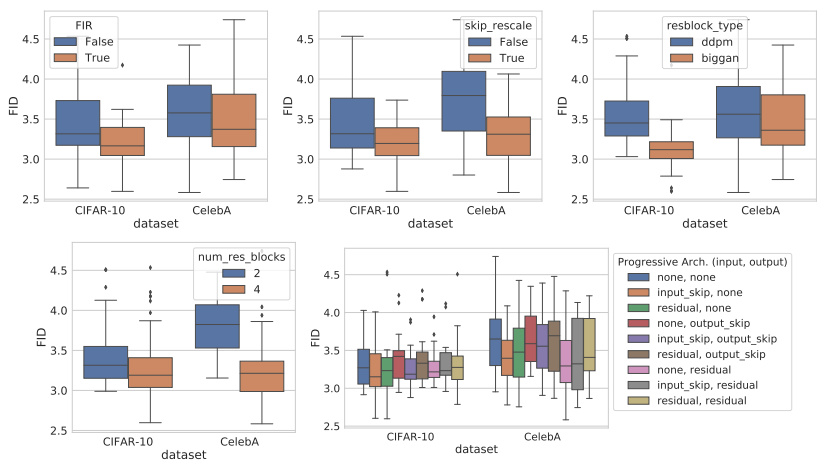
\includegraphics[width=0.8\linewidth]{figures/10.png}
    \caption{Hiệu ứng của các thành phần khác nhau của kiến trúc cho các mô hình dựa trên điểm số được huấn luyện với VE SDE}
    \label{fig:10}
\end{figure}

Kiến trúc của các mô hình chủ yếu dựa trên \citep{ho2020denoising}.
Ta giới thiệu thêm các thành phần để cực đại hóa các cải thiện tiềm năng cho mô hình dựa trên điểm số.

\begin{enumerate}
    \item Upsampling and downsampling ảnh với khử răng cưa dựa trên bộ lọc đáp ứng xung hữu hạn (FIR) \citep{zhang2019making}.
    Ta thực thi và các tham số như trong StyleGAN-v2 \citep{karras2020analyzing}.
    \item Chia các skip connection bằng $1/\sqrt{2}$.
    Điều này đã chứng minh hiệu quả trong nhiều mô hình GAN bao gồm ProgressiveGAN \citep{karras2018progressive}, StyleGAN \citep{karras2019style} và StyleGAN-2 \citep{karras2020analyzing}.
    \item Thay thế các residual block ban đầu trong DDPM bởi các residual block trong BigGAN \citep{brock2018large}.
    \item Tăng số residual block trên một độ phân giải từ 2 lên 4.
    \item Kết hợp kiến trúc tăng trưởng dần dần.
    Ta xét hai kiến trúc tăng trưởng dần dần cho đầu vào: nhảy cách đầu vào và phần dư, và hai kiến trúc cho đầu ra: nhảy cách đầu ra và phần dư.
    Các kiến trúc này được định nghĩa và thực thi theo StyleGAN-2.
\end{enumerate}

Ta cũng thử nghiệm learning rate, một thủ thuật được sử dụng trong các mô hình nổi tiếng như ProgressiveGAN \citep{karras2018progressive} và StyleGAN \citep{karras2019style}.
Tuy nhiên, ta nhận thấy thủ thật này ảnh hưởng tại giai đoạn đầu của thử nghiệm và vì vậy quyết định không tiếp tục thử nghiệm với thủ thuật này.

Tham số của Exponential moving average (EMA) ảnh hưởng lớn đến hiệu năng của mô hình.
Mô hình được huấn luyện với xáo trộn VE, ta thấy 0.999 tốt hơn 0.9999, với mô hình được huấn luyện với xáo trộn VP thì ngược lại.
Vì vậy ta sử dụng tham số EMA là 0.999 và 0.9999 tương ứng cho VE và VP.

\subsection{Kết quả trên tập CIFAR-10} \label{H.2}

Tất cả các thành phần kiến trúc đã được giới thiệu ở treen có thể cải thiện hiệu năng của mô hình dựa trên điểm số được huấn luyện với VE SDE, được minh họa ở hình \ref{fig:10}.
Box plot thể hiện sự quan trọng của từng thành phần khi khi thành phần khác biến đổi tự do.
Trên cả hai tập CIFAR-10 và CelebA, các thành phần bổ sung ta thử nghiệm luôn luôn cải thiện hiệu năng trung bình trên VE SDEs.
Đối với tương trưởng dần dần, không thấy rõ ràng sự kết hợp của các cấu hình không phỉa lúc nào cũng cho kết quả tốt nhất, nhưng kết quả thừng tốt hơn nếu không sử dụng kiến trúc tăng trưởng dần dần.
Mô hình dựa trên điểm số tốt nhất dành cho VE SDE 1) sử dụng FIR upsampling/downsampling, 2) thay đổi tỷ lệ skip connection, 3) sử dụng residual block của BigGAN, 4) sử dụng 4 residual block trên từng một độ phân giải thay vì 2, và 5) sử dụng "phần dư" cho đầu vào và không sử dụng kiến trúc tăng trưởng dần dần cho đầu ra.
Ta gọi mô hình này là NCSN++, theo quy ước đặt tên của mô hình SMLD \citep{song2019generative, song2020improved}

Ta theo thủ tục tương tử để kiểm tra các thành phần kiến trúc cho VP SDEs, ngoại trừ bỏ qua các thử nghiệm trên CelebA vì giới hạn nguồn lực tính toán.
Kiến trúc NCSN++ làm việc tốt cho VP SDEs, và đứng thứ 4 trong 144 cấu hình.
Cấu hình tốt nhất, tuy nhiên có cấu trúc hơi khác, không sử dụng FIR upsampling/downsampling và không có kiến trúc tăng trưởng dần dần như NCSN++.
Ta gọi mô hình này là DDPM++, được đặt theo quy ước đặt tên của \citep{ho2020denoising}.

Mô hình NCSN++ cơ bản với 4 residual block trên một độ phân giải đạt được FID là 2.45 trên tập CIFAR-10,
trong khi mô hình DDPM++ đạt FID là 2.78.
Để khớp với các quy ước được sử dụng trong \citep{karras2018progressive,song2019generative} và \citep{ho2020denoising}, ta báo cáo giá trị FID nhỏ nhất trên toàn bộ quá trình huấn luyện thay vì giá trị FID trung bình trên các checkpoint sau 0.5 triệu vòng lặp (được sử dụng để so sánh các mô hình khác nhau của VE SDEs) hoặc giữa 0.25 triệu và 0.5 triệu bước lặp (được sử dụng so sánh các mô hình VP SDE) trong tìm kiếm các kiến trúc phù hợp.

Được chuyển từ hàm mục tiêu rời rạc sang hàm mục tiêu liên tục trong công thức \ref{eq:7} cũng làm cải thiện các giá trị FID cho toàn bộ các phương trình SDE.
Để đặt điều kiện trên mô hình NCSN++ trên biến thời gian liên tục, ta thay đổi positional embedding thành Fourier feature embedding \citep{tancik2020fourier}.
Các tham số tỷ lệ của Fourier feature embedding ngẫu nhiên được đặt cố định là 16.
Ta cũng giảm số bước huấn luyện về 0.95 triệu bước để làm giảm quá khớp.
Thay đổi này cải thiện FID trên tập CIFAR-10 từ 2.45 thành 2.38 cho NCSN++ được huấn luyện với VE SDE, kết quả tạo ra một mô hihf gọi là NCSN++ cont.
Hơn nữa, ta có thể cải thiện FID từ 2.38 trở thành 2.20 bằng cách tăng gấp đôi số residual block trên một độ phân giải cho NCSN++ cont, kết quả tạo ra một mô hình tên là NCSN++ cont (deep).
Tất cả các kết quả định lượng được tổng hợp ở bảng \ref{tab:3}, ta cung cấp các mẫu ngẫu nhiên từ mô hình tốt nhất ở hình 


Tương tự, ta có thể tạo điều kiện trên mô hình DDPM++ cho bước thời gian liên tục, kết quả tạo ra mô hình DDPM++ cont.
Khi huấn luyện với VP SDE, ta cải thiện FID từ 2.78 của DDPM++ thành 2.55.
Khi huấn luyện với sub-VP SDE, ta thu được FID là 2.61.
Để thu được kết quả tốt hơn, ta sử dụng bộ giải Euler - Maruyama là bộ dự đoán cho mô hình được huấn luyện liên tục, thay vì bộ dự đoán ancestral sampling hoặc bộ dự đoán khuếch tán ngược.
Bở vì chiến lược rời rạc hóa của phương pháp DDPM gốc không hớp với phương sai của quá trình liê tục khi $t \rightarrow 0$ làm ảnh hưởng đáng kể FID.
Được tổng hợp ở bảng \ref{tab:2}, giá trị độ hợp lý là 3.21 và 3.05 bits/dim cho lần lượt VP và sub-VP SDEs.
Tăng gấp đôi độ sâu và huấn luyện với 0.95 triệu bước lặp, ta cải thiện cả FID và bits/dim cho cả VP và sub-VP SDEs, tạo nên mô hình DDPM++ cont (deep).
Giá trị điểm số FID là 2.41 cho cả VP và VP SDE.
Khi huấn luyện VP SDE, đạt được độ hợp lý là 2.99 bits/dim.
Tất cả các độ hợp lý được tính trên checkpoint cuối cùng của quá trình huấn luyện.

\begin{figure}[h!]
    \centering
    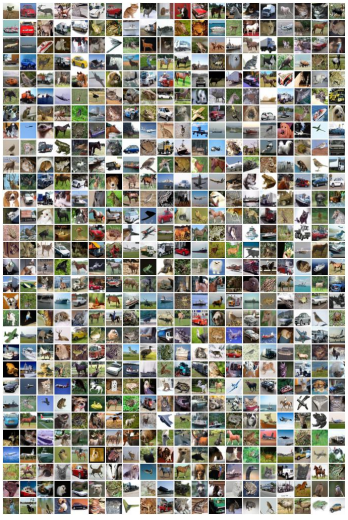
\includegraphics[width=0.7\textwidth]{figures/11.png}
    \caption{Các mẫu CIFAR-10 được tạo ra không có điều kiện từ mô hình NCSN++ cont (deep, VE)}
    \label{fig:11}
\end{figure}

\begin{figure}[h!]
    \centering
    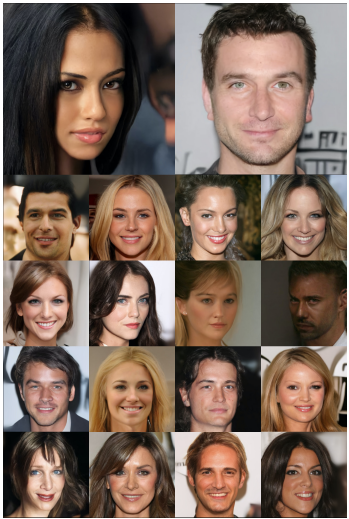
\includegraphics[width=0.7\textwidth]{figures/12.png}
    \caption{Các mẫu trên tập CelebA-HQ 1024$\times$1024 từ mô hình NCSN++ được điều chỉnh và huấn luyện với VE SDE.}
    \label{fig:12}
\end{figure}

\subsection{Các ảnh có độ phân giải cao} \label{H.3}

Được khích lệ từ thành công của NCSN++ trên tập CIFAR-10, ta tiếp tục thử nghiệm trên tập CelebA-HQ 1024$\times$1024 \citep{karras2018progressive}, một bài toán trước đây chỉ có thể làm được với một số mô hình GAN và VQ-VAE-2 \citep{razavi2019generating}.
Ta sử dụng batch size là 8, tăng tỷ số EMA lên thành 0.9999 và huấn luyện mô hình tương tự với NCSN++ với hàm mục tiêu liên tục trong công thức \ref{eq:7} trong 2.4 triệu bước lặp.
Ta sử dụng bộ lấy mẫu PC rời rạc hóa tại 2000 bước với bộ dự đoán khuếch tán ngược, một bước Langevin trên từng bước dự đoán cập nhật là tham số signal-to-noise là 0.15.
Tham số tỷ lệ cho Fourier feature embedding ngẫu nhiên được cố định là 16.
Ta sử dụng kiến trúc tăng trưởng dần dần nhảy cách đầu vào cho đầu vào và kiến trúc tăng trưởng dần dần nhảy cách đầu ra cho đầu ra.
Ta cung cấp một vài mẫu trong hình \ref{fig:12}.
Mặc dù các mẫu không hoàn hảo (có một vài vết trên khuôn mặt), ta vẫn tin rằng các kết quả này khích lệ và có thể thể hiện tính mở rộng của cách tiếp cận.
Các công trình tiếp theo tập trung vào các kiến trúc hiệu quả hơn để làm tiến bộ đáng kể khả năng của mô hình sinh dựa trên điểm số trên bài toán này.

\section{Sinh mẫu có điều khiển} \label{I}

Ta xét phương trình SDE thuận với dạng tổng quát sau:

\begin{equation*}
    d \bold{x} = \bold{f}(\bold{x}, t) dt + \bold{G} (\bold{x}, t) d\bold{w}
\end{equation*}

và giả sử phân phối trạng thái ban đầu là $p_0(\bold{x}(0) \vert \bold{y})$.
Hàm mật độ tại thời điểm $t$ là $p_t(\bold{x}(t) \vert \bold{y})$ được lấy điều kiện trên $\bold{y}$.
Vì vậy, sử dụng \citep{anderson1982reverse}, phương trình SDE đảo ngược thời gian thu được bởi:

\begin{equation} \label{eq:48}
    d \bold{x} = \lbrace \bold{f}(\bold{x}, t) - \nabla . \lbrack \bold{G}(\bold{x}, t) \bold{G}(\bold{x}, t)^T \rbrack - \bold{G}(\bold{x}, t)\bold{G}(\bold{x}, t)^T \nabla_{\bold{x}} \log p_t (\bold{x} \vert \bold{y}) \rbrace dt + \bold{G}(\bold{x}, t)  d \bar{\bold{w}}
\end{equation}

Khi $p_t (\bold{x} \vert \bold{y}) \propto p_t(\bold{x}(t)) p(\bold{y} \vert \bold{x}(t))$, hàm điểm số $\nabla_{\bold{x}} \log p_t (\bold{x}(t) \vert \bold{y})$ có thể được tính dễ dàng bởi công thức:

\begin{equation} \label{eq:49}
    \nabla_{\bold{x}} \log p_t (\bold{x}(t) \vert \bold{y}) = \nabla_{\bold{x}} \log p_t(bold{x}(t)) + \nabla_{\bold{x}} \log p(\bold{y} \vert \bold{x}(t))
\end{equation}

Thành phần này đóng góp vào phương trình SDE đảo ngược thời gian ở công thức \ref{eq:14} như một trường hợp đặc biệt.
Tất cả các phương pháp lấy mẫu ta đã thảo luận có thể được áp dụng cho phương trình SDE đảo ngược thời gian có điều kiện cho sinh mẫu dữ liệu.

\subsection{Lấy mẫu trên điều kiện lớp} \label{I.1}

Khi $\bold{y}$ biểu diễn nhãn lớp, ta có thể huấn luyện một bộ phân lớp phụ thuộc vào thời gian $p_t(\bold{y} \vert \bold{x}(t))$ cho lấy mẫu có điều kiện trên lớp.
Khi phương trình SDE thuận là dễ áp dụng, ta có thể dễ dàng áp dụng một cặp dữ liệu huấn luyện $(\bold{x}(t), \bold{y})$ bừng cách đầu tiên lấy mẫu $(\bold{x}(0), \bold{y})$ từ tập dữ liệu và thu được $\bold{x}(t) \sim p_{0t}(\bold{x}(t) \vert \bold{x}(0))$.
Sau đó ta có thể sử dụng sự pha trộn của hàm tổn thất cross-entropy trên các bước thời gian khác nhau như công thức \ref{eq:7} để huấn luyện bộ phân loại phụ thuộc vào thời gian $p_t(\bold{y} \vert \bold{x}(t))$.

Để kiểm chứng ý tưởng này, ta huấn luyện một mô hình Wide ResNet \citep{zagoruyko2016wide} (Wide-ResNet-28-10) trên tập CIFAR-10 với xáo trộn VE.
Bộ phân loại được lấy điều kiện trên $\log \sigma_i$ sử dụng Fourier features ngẫu nhiên \citep{tancik2020fourier} và hàm mục tiêu là tổng của hàm mất mát cross-entropy được lấy mẫu trên nhiều ngưỡng khác nhau.
Ta cung cấp một đồ thị để hiển thị độ chính xác của bộ phân loại này trên các ngưỡng nhiễu trong hình \ref{fig:13}.
Mô hình dựa trên điểm số là một NCSN++ (4 residual block trên một độ phân giải) trong bảng \ref{tab:3} và ta sinh ra các mẫu sử dụng bộ lấy mẫu PC với 2000 bước rời rạc hóa.
Các mẫu có điều kiện trên lớp được cung cấp ở hình \ref{fig:4} và một tập mở rộng của các mẫu có điều kiện được hiển thị ở hình \ref{fig:13}.


\begin{figure}[h!]
    \centering
    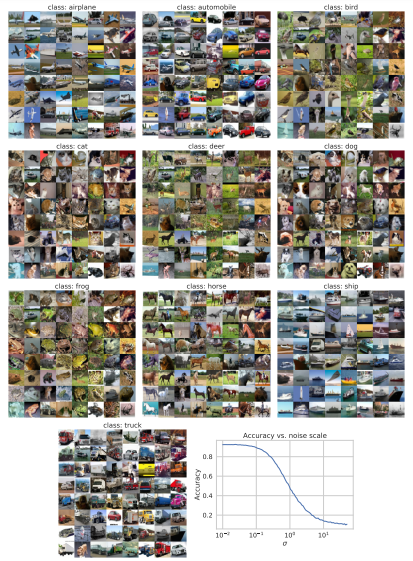
\includegraphics[height=0.8\textheight]{figures/13.png}
    \caption{Các ảnh được tạo ra từ điều kiện trên lớp bằng cách giải phương trình SDE đảo ngược thời gian có điều kiện với bộ lấy mẫu PC.
    Đường cong thể hiện độ chính xác của bộ phân loại điều kiện khi bị nhiễu trên các ngưỡng nhiễu khác nhau.}
    \label{fig:13}
\end{figure}

\subsection{Xóa môt phần ảnh} \label{I.2}

Xóa một phần ảnh là một trường hợp đặc biệt của lấy mẫu có điều kiện.
Ký hiệu $\Omega(\bold{x})$ và $\bar{\Omega}(\bold{x})$ là số chiều được biết hoặc không biết của $\bold{x}$,
đặt $\bold{f}_{\Omega}(., t)$ và $\bold{G}_{\Omega}(., t)$ ký hiệu $\bold{f}(., t)$ và $\bold{G}(., t)$ là trong trường hợp không biết số chiều.
Cho VE/VP SDEs, hệ số trôi $bold{f}(., t)$ là tính theo từng phần tử và hệ số phân tán $\bold{G}(., t)$ là ma trận đường chéo.
Khi $\bold{f}(., t)$ là theo từng phần tử, $\bold{f}_{\Omega}(., t)$ ký hiệu hàm từng phần tử tương tự chỉ áp dụng cho số chiều không biết.
Khi $\bold{G}(., t)$ là ma trận đường chéo, $\bold{G}_{\bar{\Omega}}(., t)$ ký hiệu là ma trận con cho trường hợp số chiều không biết.

Để việc xóa một phần ảnh, mục đích của ta là lấy mẫu từ $p(\bar{\Omega}(\bold{x}(0)) \vert \Omega(\bold{x}(0))=\bold{y})$.
Định nghĩa một quá trình khuếch tán mới $\bold{z} = \bar{\Omega}(\bold{x}(t))$ và chú ý rằng phương trình SDE cho $\bold{z}(t)$ có thể được viết dưới dạng:

\begin{equation*}
    d \bold{z} = \bold{f}_{\bar{\Omega}} (\bold{z}, t) + \bold{G}_{\bar{\Omega}} (\bold{z}, t) d \bold{w}
\end{equation*}

Phương trình SDE đảo ngược thời gian được lấy điều kiện trên $\Omega(\bold{x}(0))=\bold{y}$ được cho bởi công thức

\begin{equation*}
    d \bold{z} = \lbrace \bold{f}_{\bar{\Omega}} (\bold{z}, t) - \nabla . \lbrack \bold{G}_{\bar{\Omega}}(\bold{z}, t)\bold{G}_{\bar{\Omega}}(\bold{z}, t)^T \rbrack - \bold{G}_{\bar{\Omega}}(\bold{z}, t)\bold{G}_{\bar{\Omega}}(\bold{z}, t)^T \nabla_{\bold{z}} \log p_t (\bold{z} \vert \Omega(\bold{z}(0))=\bold{y}) \rbrace dt + \bold{G}_{\bar{\Omega}}(\bold{z}, t) d \bar{\bold{w}}
\end{equation*}

Mặc dù $p_t(\bold{z}(t) \vert \Omega(\bold{x}(0))=\bold{y})$ về cơ bản là khó thu được tường minh, nhưng có thể xấp xỉ được.
Đặt $A$ là sự kiện $\Omega(\bold{x}(0))=\bold{y}$. Ta có:

\begin{equation*}
    \begin{aligned}
        p_t (\bold{z}(t) \vert \Omega(\bold{x}(0))=\bold{y})=p_t(\bold{z}(t) \vert A) &= \int p_t(\bold{z}(t) \vert \Omega(\bold{x}(t)), A)p_t(\Omega(\bold{x}(t)) \vert A) d \Omega (\bold{x}(t)) \\
        &= \mathbb{E}_{p_t(\Omega(\bold{x}(t)) \vert A)} \lbrack p_t(\bold{z}(t) \vert \Omega(\bold{x}(t)), A) \rbrack \\
        &\approx \mathbb{E}_{p_t(\Omega(\bold{x}(t)) \vert A)} \lbrack p_t(\bold{z}(t) \vert \Omega(\bold{x}(t))) \rbrack \\
        &\approx p_t(\bold{z}(t) \vert \hat{\Omega}(\bold{x}(t)))
    \end{aligned}
\end{equation*}

với $\hat{\Omega}(\bold{x}(t))$ là một mẫu ngẫu nhiên từ $p_t(\Omega(\bold{x}(t)) \vert A)$ thường là một phân phối rất dễ dàng thu được.
Vì vậy:

\begin{equation*}
    \begin{aligned}
        \nabla_{\bold{z}} \log p_t(\bold{z}(t) \vert \Omega(\bold{x}(0))=\bold{y}) &\approx \nabla_{\bold{z}} \log p_t(\bold{z}(t) \vert \hat{\Omega}(\bold{x}(t)))\\
        &= \nabla_{\bold{z}} \log p_t([\bold{z}(t); \hat{\Omega}(\bold{x}(t))])
    \end{aligned}
\end{equation*}

với $[\bold{z}(t); \hat{\Omega}(\bold{x}(t))]$ ký hiệu một vector $\bold{u}(t)$ sao cho $\Omega(\bold{u}(t))=\hat{\Omega}(\bold{x}(t))$ và $\bar{\Omega}(\bold{u}(t))=\bold{z}(t)$ và đồng nhất thức đúng vì $\nabla_{\bold{z}} \log p_t ([\bold{z}(t); \hat{\Omega}(\bold{x}(t))])=\nabla_{\bold{z}} \log p_t (\bold{z}(t) \vert \hat{\Omega}(\bold{x}(t))) + \nabla_{\bold{z}} \log p(\hat{\Omega}(\bold{x}(t)))=\nabla_{\bold{z}} \log p_t (\bold{z}(t) \vert \hat{\Omega}(\bold{x}(t)))$

Ta biểu diễn một số kết quả inpainting ở hình \ref{fig:14} và hình \ref{eq:15}.

\subsection{Bài toán tô màu} \label{I.3}

Bài toán tô màu là trường hợp đặc biệt của xóa một phần ảnh, ngoại trừ việc biết trước chiều dữ liệu.
Ta có thể tách chiều dữ liệu sử dụng một phép biến đổi tuyến tính trực giao hóa để ánh xạ ảnh xám thành các kênh riêng biệt trong một không gian khác, sau đó thực hiện xóa một ảnh ảnh để hoàn thành các kênh khác trước khi biến đổi mọi thứ về không gian ảnh ban đầu.
Ma trận trực giao ta sử dụng để tách các kênh màu là:

\begin{equation*}
    \begin{pmatrix}
        0.577 & -0.816 & 0 \\
        0.577 & 0.408 & 0.707 \\
        0.577 & 0.408 & -0.707
    \end{pmatrix}
\end{equation*}

Bởi vì các phép biến đổi đều là các ma trận trực giao, quá trình Wiener chuẩn tắc $\bold{w}(t)$ vẫn là một quá trình Wiener chuẩn tắc trong không gian đã được biến đổi, cho phép chúng ta xây dựng một phương trình SDE và sử dụng phương pháp xóa ảnh tương tự như trong phụ lục .
Ta cung các một tập các kết quả tô màu ở hình \ref{fig:16} và hình \ref{fig:17}

\subsection{Giải các bài toán ngược tổng quát} \label{I.4}

Giả sử ta có hai biến ngẫu nhiên $\bold{x}$ và $\bold{y}$ và ta biết quá trình thuận của sinh ra $\bold{y}$ từ $\bold{x}$ được cho bởi $p(\bold{y} \vert \bold{x})$.
Bài toán ngược là thu được $\bold{x}$ từ $\bold{y}$ và sinh ra các mẫu từ phân phối $p(\bold{x} \vert \bold{y})$.
Về mặt nguyên lý, ta có thể ước lượng phân phối tiên nghiệm $p(\bold{x})$ và thu được $p(\bold{x} \vert \bold{y})$ sử dụng quy tắc Bayes: $p(\bold{x} \vert \bold{y})=p(\bold{x})p(\bold{y} \vert \bold{x}) / p(\bold{y})$.
Tuy nhiên trong thực tế, ta ước lượng phân phối tiên nghiệm và thực hiện suy luận Bayes là không dễ dàng.

Tận dụng công thức \ref{eq:48}, mô hình sinh dựa trên điểm số cung cấp một cách để giải bài toán ngược.
Giả sử ta có một quá trình khuếch tán $\lbrace \bold{x}(T) \rbrace_{t=0}^T$ được tạo ra bằng cách gây xáo trộn $\bold{x}$ bằng một phương trình SDE và một mô hình dựa trên điểm số $\bold{s}_{\boldsymbol{\theta}^{\ast}}(\bold{x}, t)$ được huấn luyện để xấp xỉ $\nabla_{\bold{x}} p_t(\bold{x}(t))$.
Một khi ta đã có ước lượng của $\nabla_{\bold{x}} \log p_t(\bold{x}(t) \vert \bold{y})$, ta có thể mô phỏng phương trình SDE đảo ngược thời gian trong công thức ref{eq:48} để lấy mẫu từ phân phối $p_0(\bold{x}(0) \vert \bold{y})=p(\bold{x} \vert \bold{y})$.
Để thu được ước lượng này, ta trước hết cần quan sát rằng:

\begin{equation*}
    \nabla_{\bold{x}} p_t (\bold{x}(t) \vert \bold{y}) = \nabla_{\bold{x}} \log \int p_t(\bold{x}(t) \vert \bold{y}(t), \bold{y}) p(\bold{y}(t) \vert \bold{y}) d \bold{y}(t)
\end{equation*}

với $\bold{y}(t)$ được định nghĩa thông qua $\bold{x}(t)$ và quá trình thuận $p(\bold{y}(t) \vert \bold{x}(t))$. Ta giả định hai điều kiện:

\begin{itemize}
    \item $p(\bold{y}(t) \vert \bold{y})$ dễ thu được.
    Ta có thể thu được phân phối này từ tương tác giữa quá trình thuận  và phương trình SDE, giống như trường hợp xóa một phần ảnh hoặc tô màu ảnh.
    \item $p_t(\bold{x}(t) \vert \bold{y}(t), \bold{y}) \approx p_t(\bold{x}(t) \vert \bold{y}(t))$.
    Với $t$ nhỏ, $\bold{y}(t)$ gần như bằng với $\bold{y}$ nên xấp xỉ trên gần đúng.
    Với $t$ lớn, $\bold{y}$ trở nên rất xa với $\bold{x}(t)$ trong xích Markov,
    và ảnh hưởng nhỏ hơn trên $\bold{x}(t)$.
    Hơn nữa, sai số xấp xỉ cho $t$ lớn ít quan trọng cho mẫu được sinh ra khi mà nó được sử dụng ở ban đầu ở quá trình lấy mẫu.
\end{itemize}

Với hai giả định trên, ta có:

\begin{equation} \label{eq:50}
    \begin{aligned}
        \nabla_{\bold{x}} \log p_t (\bold{x}(t) \vert \bold{y}) &\approx \nabla_{\bold{x}} \log \int p_t(\bold{x}(t) \vert \bold{y}(t)) p(\bold{y}(t) \vert \bold{y}) d\bold{y} \\
        &\approx \nabla_{\bold{x}} \log p_t(\bold{x}(t) \vert \hat{\bold{y}}(t)) \\
        &= \nabla_{\bold{x}} \log p_t(\bold{x}(t)) + \nabla_{\bold{x}} \log p_t (\hat{\bold{y}}(t) \vert \bold{x}(t)) \\
        &\approx \bold{s}_{\boldsymbol{\theta}^{\ast}} (\bold{x}(t), t) + \nabla_{\bold{x}} \log p_t (\hat{\bold{y}}(t) \vert \bold{x}(t))
    \end{aligned}
\end{equation}

với $\hat{\bold{y}}(t)$ là một mẫu từ $p(\bold{y}(t) \vert \bold{y})$.
Bây giờ ta có thể thế công thức \ref{eq:50} vào công thức \ref{eq:48} và giải phương trình SDE đảo ngược thời gian kết quả để tạo ra mẫu dữ liệu từ $p(\bold{x} \vert \bold{y})$.

\begin{figure}[h!]
    \centering
    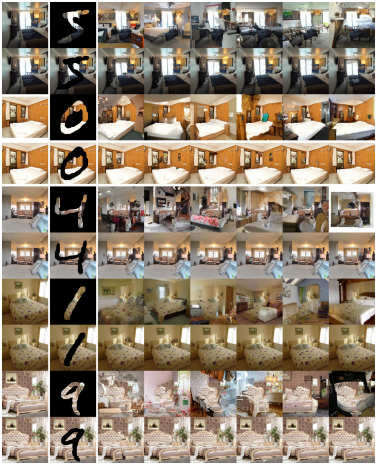
\includegraphics[width=0.8\linewidth]{figures/14.png}
    \caption{Các kết quả inpainting cho các ảnh bedroom 256 $\times$ 256}
    \label{fig:14}
\end{figure}

\begin{figure}[h!]
    \centering
    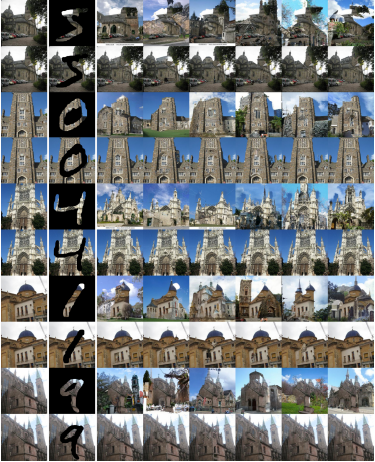
\includegraphics[width=0.8\linewidth]{figures/15.png}
    \caption{Các kết quả inpainting cho các ảnh church 256 $\times$ 256}
    \label{fig:15}
\end{figure}

\begin{figure}[h!]
    \centering
    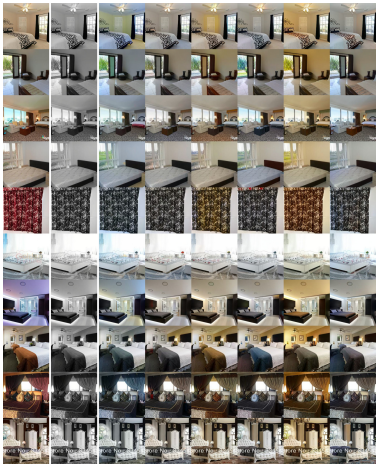
\includegraphics[width=0.8\linewidth]{figures/16.png}
    \caption{Các kết quả tô màu cho các ảnh bedroom 256 $\times$ 256}
    \label{fig:16}
\end{figure}

\begin{figure}[h!]
    \centering
    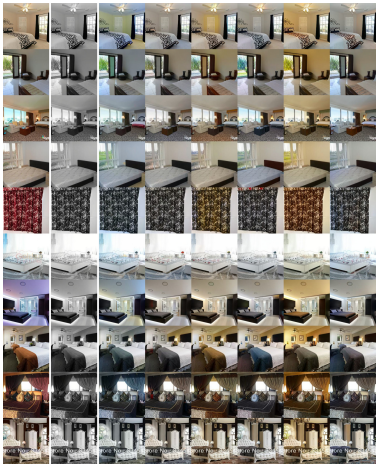
\includegraphics[width=0.8\linewidth]{figures/16.png}
    \caption{Các kết quả tô màu cho các ảnh church 256 $\times$ 256}
    \label{fig:17}
\end{figure}
\end{document}